% **************************************************************************************************************
% To Do:
%    * [low] => Cites / bibliography
% **************************************************************************************************************
\documentclass[titlepage, numbers=noenddot, headinclude,
                %headlines,% letterpaper a4paper %%%openright,%%%
                footinclude=true,cleardoublepage=empty,abstractoff, % <--- obsolete, remove (todo)
                BCOR=5mm, letterpaper,fontsize=11.5pt,%11pt,a4paper,%
                %ngerman,american%
                ]{scrreprt}

%********************************************************************
% Note: Make all your adjustments in here
%*******************************************************
%\bibliographystyle{plain}
\bibliographystyle{alpha}
%!TEX root = Base.tex

% ****************************************************************************************************
% classicthesis-config.tex 
% formerly known as loadpackages.sty, classicthesis-ldpkg.sty, and classicthesis-preamble.sty 
% Use it at the beginning of your ClassicThesis.tex, or as a LaTeX Preamble 
% in your ClassicThesis.{tex,lyx} with %!TEX root = Base.tex

% ****************************************************************************************************
% classicthesis-config.tex 
% formerly known as loadpackages.sty, classicthesis-ldpkg.sty, and classicthesis-preamble.sty 
% Use it at the beginning of your ClassicThesis.tex, or as a LaTeX Preamble 
% in your ClassicThesis.{tex,lyx} with %!TEX root = Base.tex

% ****************************************************************************************************
% classicthesis-config.tex 
% formerly known as loadpackages.sty, classicthesis-ldpkg.sty, and classicthesis-preamble.sty 
% Use it at the beginning of your ClassicThesis.tex, or as a LaTeX Preamble 
% in your ClassicThesis.{tex,lyx} with \input{classicthesis-config}
% ****************************************************************************************************  
% If you like the classicthesis, then I would appreciate a postcard. 
% My address can be found in the file ClassicThesis.pdf. A collection 
% of the postcards I received so far is available online at 
% http://postcards.miede.de
% ****************************************************************************************************

% ****************************************************************************************************
% 1. Configure classicthesis for your needs here, e.g., remove "drafting" below 
% in order to deactnivate the time-stamp on the pages
% ****************************************************************************************************
\PassOptionsToPackage{eulerchapternumbers,listings,drafting,%
				 pdfspacing, eulermath, 
         %floatperchapter,%linedheaders,% beramono
				 parts}{classicthesis}										
% ********************************************************************
% Available options for classicthesis.sty 
% (see ClassicThesis.pdf for more information):
% drafting
% parts nochapters linedheaders
% eulerchapternumbers beramono eulermath pdfspacing minionprospacing
% tocaligned dottedtoc manychapters
% listings floatperchapter subfig
% ********************************************************************

% ********************************************************************
% Triggers for this config
% ******************************************************************** 
\usepackage{ifthen}
\newboolean{enable-backrefs} % enable backrefs in the bibliography
\setboolean{enable-backrefs}{false} % true false
% ****************************************************************************************************


% ****************************************************************************************************
% 2. Personal data and user ad-hoc commands
% ****************************************************************************************************
\newcommand{\myTitle}{Avance de tesis\xspace}
\newcommand{\mySubtitle}{:)\xspace}
\newcommand{\myDegree}{Ingeniero (Ing.)\xspace}
\newcommand{\myName}{Rafael de Jes\'us Robledo Ju\'arez \xspace}
\newcommand{\myProf}{Dr. Salvador Ruíz Correa \xspace}
\newcommand{\myOtherProf}{Prof. 1\xspace}
\newcommand{\mySupervisor}{Prof. 2\xspace}
\newcommand{\myFaculty}{Centro de Investigaci\'on en Matem\'aticas\xspace}
\newcommand{\myDepartment}{Departamento de Ciencias de la Computaci\'on\xspace}
\newcommand{\myUni}{\xspace}
\newcommand{\myLocation}{Guanajuato, México\xspace}
\newcommand{\myTime}{Noviembre 2013\xspace}
\newcommand{\myVersion}{version 0.85\xspace}

% ********************************************************************
% Setup, finetuning, and useful commands
% ********************************************************************
\newcounter{dummy} % necessary for correct hyperlinks (to index, bib, etc.)
\newlength{\abcd} % for ab..z string length calculation
\providecommand{\mLyX}{L\kern-.1667em\lower.25em\hbox{Y}\kern-.125emX\@}
\newcommand{\ie}{i.\,e.}
\newcommand{\Ie}{I.\,e.}
\newcommand{\eg}{e.\,g.}
\newcommand{\Eg}{E.\,g.}
% ****************************************************************************************************

% ****************************************************************************************************
% 3. Loading some handy packages
% ****************************************************************************************************
% ******************************************************************** 
% Packages with options that might require adjustments
% ******************************************************************** 
\PassOptionsToPackage{utf8}{inputenc}
 \usepackage{inputenc}				

%\PassOptionsToPackage{ngerman,american}{babel}   % change this to your language(s)
% Spanish languages need extra options in order to work with this template
\PassOptionsToPackage{spanish,es-lcroman}{babel}
 \usepackage{babel}					

\PassOptionsToPackage{square,numbers}{natbib}
 \usepackage{natbib}				

\PassOptionsToPackage{fleqn}{amsmath}		% math environments and more by the AMS 
 \usepackage{amsmath}
 
 \usepackage[spanish, fixlanguage]{babelbib}
 \bibliographystyle{babelbib}

% ******************************************************************** 
% General useful packages
% ******************************************************************** 
\PassOptionsToPackage{T1}{fontenc} % T2A for cyrillics
	\usepackage{fontenc}     
\usepackage{textcomp} % fix warning with missing font shapes
\usepackage{scrhack} % fix warnings when using KOMA with listings package          
\usepackage{xspace} % to get the spacing after macros right  
\usepackage{mparhack} % get marginpar right
\usepackage{fixltx2e} % fixes some LaTeX stuff 
\PassOptionsToPackage{printonlyused}{acronym}
	\usepackage{acronym} % nice macros for handling all acronyms in the thesis
%\renewcommand*{\acsfont}[1]{\textssc{#1}} % for MinionPro
\renewcommand{\bflabel}[1]{{#1}\hfill} % fix the list of acronyms
% ****************************************************************************************************


% ****************************************************************************************************
% 4. Setup floats: tables, (sub)figures, and captions
% ****************************************************************************************************
\usepackage{tabularx} % better tables
	\setlength{\extrarowheight}{3pt} % increase table row height
\newcommand{\tableheadline}[1]{\multicolumn{1}{c}{\spacedlowsmallcaps{#1}}}
\newcommand{\myfloatalign}{\centering} % to be used with each float for alignment
% \usepackage{caption}
\usepackage[font=small,format=plain,labelfont=bf,up,textfont=it,up]{caption}
\captionsetup{format=hang,font=small}
% \usepackage{subfig}  
% ****************************************************************************************************


% ****************************************************************************************************
% 5. Setup code listings
% ****************************************************************************************************
\usepackage{listings} 
%\lstset{emph={trueIndex,root},emphstyle=\color{BlueViolet}}%\underbar} % for special keywords
\lstset{language=[LaTeX]Tex,%C++,
    keywordstyle=\color{RoyalBlue},%\bfseries,
    basicstyle=\small\ttfamily,
    %identifierstyle=\color{NavyBlue},
    commentstyle=\color{Green}\ttfamily,
    stringstyle=\rmfamily,
    numbers=none,%left,%
    numberstyle=\scriptsize,%\tiny
    stepnumber=5,
    numbersep=8pt,
    showstringspaces=false,
    breaklines=true,
    frameround=ftff,
    frame=single,
    belowcaptionskip=.75\baselineskip
    %frame=L
} 
% ****************************************************************************************************    		   


% ****************************************************************************************************
% 6. PDFLaTeX, hyperreferences and citation backreferences
% ****************************************************************************************************
% ********************************************************************
% Using PDFLaTeX
% ********************************************************************
\PassOptionsToPackage{pdftex,hyperfootnotes=false,pdfpagelabels}{hyperref}
	\usepackage{hyperref}  % backref linktocpage pagebackref
\pdfcompresslevel=9
\pdfadjustspacing=1 
\PassOptionsToPackage{pdftex}{graphicx}
	\usepackage{graphicx} 

% ********************************************************************
% Setup the style of the backrefs from the bibliography
% (translate the options to any language you use)
% ********************************************************************
\newcommand{\backrefnotcitedstring}{\relax}%(Not cited.)
\newcommand{\backrefcitedsinglestring}[1]{(Cited on page~#1.)}
\newcommand{\backrefcitedmultistring}[1]{(Cited on pages~#1.)}
\ifthenelse{\boolean{enable-backrefs}}%
{%
		\PassOptionsToPackage{hyperpageref}{backref}
		\usepackage{backref} % to be loaded after hyperref package 
		   \renewcommand{\backreftwosep}{ and~} % separate 2 pages
		   \renewcommand{\backreflastsep}{, and~} % separate last of longer list
		   \renewcommand*{\backref}[1]{}  % disable standard
		   \renewcommand*{\backrefalt}[4]{% detailed backref
		      \ifcase #1 %
		         \backrefnotcitedstring%
		      \or%
		         \backrefcitedsinglestring{#2}%
		      \else%
		         \backrefcitedmultistring{#2}%
		      \fi}%
}{\relax}    

% ********************************************************************
% Hyperreferences
% ********************************************************************
\hypersetup{%
    %draft,	% = no hyperlinking at all (useful in b/w printouts)
    colorlinks=true, linktocpage=true, pdfstartpage=3, pdfstartview=FitV,%
    % uncomment the following line if you want to have black links (e.g., for printing)
    %colorlinks=false, linktocpage=false, pdfborder={0 0 0}, pdfstartpage=3, pdfstartview=FitV,% 
    breaklinks=true, pdfpagemode=UseNone, pageanchor=true, pdfpagemode=UseOutlines,%
    plainpages=false, bookmarksnumbered, bookmarksopen=true, bookmarksopenlevel=1,%
    hypertexnames=true, pdfhighlight=/O,%nesting=true,%frenchlinks,%
    urlcolor=webbrown, linkcolor=RoyalBlue, citecolor=webgreen, %pagecolor=RoyalBlue,%
    %urlcolor=Black, linkcolor=Black, citecolor=Black, %pagecolor=Black,%
    pdftitle={\myTitle},%
    pdfauthor={\textcopyright\ \myName, \myUni, \myFaculty},%
    pdfsubject={},%
    pdfkeywords={},%
    pdfcreator={pdfLaTeX},%
    pdfproducer={LaTeX with hyperref and classicthesis}%
}   

% ********************************************************************
% Setup autoreferences
% ********************************************************************
% There are some issues regarding autorefnames
% http://www.ureader.de/msg/136221647.aspx
% http://www.tex.ac.uk/cgi-bin/texfaq2html?label=latexwords
% you have to redefine the makros for the 
% language you use, e.g., american, ngerman
% (as chosen when loading babel/AtBeginDocument)
% ********************************************************************
\makeatletter
\@ifpackageloaded{babel}%
    {%
       \addto\extrasamerican{%
					\renewcommand*{\figureautorefname}{Figure}%
					\renewcommand*{\tableautorefname}{Table}%
					\renewcommand*{\partautorefname}{Part}%
					\renewcommand*{\chapterautorefname}{Chapter}%
					\renewcommand*{\sectionautorefname}{Section}%
					\renewcommand*{\subsectionautorefname}{Section}%
					\renewcommand*{\subsubsectionautorefname}{Section}% 	
				}%
       \addto\extrasngerman{% 
					\renewcommand*{\paragraphautorefname}{Absatz}%
					\renewcommand*{\subparagraphautorefname}{Unterabsatz}%
					\renewcommand*{\footnoteautorefname}{Fu\"snote}%
					\renewcommand*{\FancyVerbLineautorefname}{Zeile}%
					\renewcommand*{\theoremautorefname}{Theorem}%
					\renewcommand*{\appendixautorefname}{Anhang}%
					\renewcommand*{\equationautorefname}{Gleichung}%        
					\renewcommand*{\itemautorefname}{Punkt}%
				}%	
			% Fix to getting autorefs for subfigures right (thanks to Belinda Vogt for changing the definition)
			\providecommand{\subfigureautorefname}{\figureautorefname}%  			
    }{\relax}
\makeatother


% ****************************************************************************************************
% 7. Last calls before the bar closes
% ****************************************************************************************************
% ********************************************************************
% Development Stuff
% ********************************************************************
\listfiles
%\PassOptionsToPackage{l2tabu,orthodox,abort}{nag}
%	\usepackage{nag}
%\PassOptionsToPackage{warning, all}{onlyamsmath}
%	\usepackage{onlyamsmath}

% ********************************************************************
% Last, but not least...
% ********************************************************************
\usepackage{classicthesis} 
% ****************************************************************************************************


% ****************************************************************************************************
% 8. Further adjustments (experimental)
% ****************************************************************************************************
% ********************************************************************
% Changing the text area
% ********************************************************************
%\linespread{1.05} % a bit more for Palatino
%\areaset[current]{312pt}{761pt} % 686 (factor 2.2) + 33 head + 42 head \the\footskip
%\setlength{\marginparwidth}{7em}%
%\setlength{\marginparsep}{2em}%

% ********************************************************************
% Using different fonts
% ********************************************************************
%\usepackage[oldstylenums]{kpfonts} % oldstyle notextcomp
%\usepackage[osf]{libertine}
%\usepackage{hfoldsty} % Computer Modern with osf
%\usepackage[light,condensed,math]{iwona}
%\renewcommand{\sfdefault}{iwona}
%\usepackage{lmodern} % <-- no osf support :-(
%\usepackage[urw-garamond]{mathdesign} <-- no osf support :-(
% ****************************************************************************************************

% ****************************************************************************************************  
% If you like the classicthesis, then I would appreciate a postcard. 
% My address can be found in the file ClassicThesis.pdf. A collection 
% of the postcards I received so far is available online at 
% http://postcards.miede.de
% ****************************************************************************************************

% ****************************************************************************************************
% 1. Configure classicthesis for your needs here, e.g., remove "drafting" below 
% in order to deactnivate the time-stamp on the pages
% ****************************************************************************************************
\PassOptionsToPackage{eulerchapternumbers,listings,drafting,%
				 pdfspacing, eulermath, 
         %floatperchapter,%linedheaders,% beramono
				 parts}{classicthesis}										
% ********************************************************************
% Available options for classicthesis.sty 
% (see ClassicThesis.pdf for more information):
% drafting
% parts nochapters linedheaders
% eulerchapternumbers beramono eulermath pdfspacing minionprospacing
% tocaligned dottedtoc manychapters
% listings floatperchapter subfig
% ********************************************************************

% ********************************************************************
% Triggers for this config
% ******************************************************************** 
\usepackage{ifthen}
\newboolean{enable-backrefs} % enable backrefs in the bibliography
\setboolean{enable-backrefs}{false} % true false
% ****************************************************************************************************


% ****************************************************************************************************
% 2. Personal data and user ad-hoc commands
% ****************************************************************************************************
\newcommand{\myTitle}{Avance de tesis\xspace}
\newcommand{\mySubtitle}{:)\xspace}
\newcommand{\myDegree}{Ingeniero (Ing.)\xspace}
\newcommand{\myName}{Rafael de Jes\'us Robledo Ju\'arez \xspace}
\newcommand{\myProf}{Dr. Salvador Ruíz Correa \xspace}
\newcommand{\myOtherProf}{Prof. 1\xspace}
\newcommand{\mySupervisor}{Prof. 2\xspace}
\newcommand{\myFaculty}{Centro de Investigaci\'on en Matem\'aticas\xspace}
\newcommand{\myDepartment}{Departamento de Ciencias de la Computaci\'on\xspace}
\newcommand{\myUni}{\xspace}
\newcommand{\myLocation}{Guanajuato, México\xspace}
\newcommand{\myTime}{Noviembre 2013\xspace}
\newcommand{\myVersion}{version 0.85\xspace}

% ********************************************************************
% Setup, finetuning, and useful commands
% ********************************************************************
\newcounter{dummy} % necessary for correct hyperlinks (to index, bib, etc.)
\newlength{\abcd} % for ab..z string length calculation
\providecommand{\mLyX}{L\kern-.1667em\lower.25em\hbox{Y}\kern-.125emX\@}
\newcommand{\ie}{i.\,e.}
\newcommand{\Ie}{I.\,e.}
\newcommand{\eg}{e.\,g.}
\newcommand{\Eg}{E.\,g.}
% ****************************************************************************************************

% ****************************************************************************************************
% 3. Loading some handy packages
% ****************************************************************************************************
% ******************************************************************** 
% Packages with options that might require adjustments
% ******************************************************************** 
\PassOptionsToPackage{utf8}{inputenc}
 \usepackage{inputenc}				

%\PassOptionsToPackage{ngerman,american}{babel}   % change this to your language(s)
% Spanish languages need extra options in order to work with this template
\PassOptionsToPackage{spanish,es-lcroman}{babel}
 \usepackage{babel}					

\PassOptionsToPackage{square,numbers}{natbib}
 \usepackage{natbib}				

\PassOptionsToPackage{fleqn}{amsmath}		% math environments and more by the AMS 
 \usepackage{amsmath}
 
 \usepackage[spanish, fixlanguage]{babelbib}
 \bibliographystyle{babelbib}

% ******************************************************************** 
% General useful packages
% ******************************************************************** 
\PassOptionsToPackage{T1}{fontenc} % T2A for cyrillics
	\usepackage{fontenc}     
\usepackage{textcomp} % fix warning with missing font shapes
\usepackage{scrhack} % fix warnings when using KOMA with listings package          
\usepackage{xspace} % to get the spacing after macros right  
\usepackage{mparhack} % get marginpar right
\usepackage{fixltx2e} % fixes some LaTeX stuff 
\PassOptionsToPackage{printonlyused}{acronym}
	\usepackage{acronym} % nice macros for handling all acronyms in the thesis
%\renewcommand*{\acsfont}[1]{\textssc{#1}} % for MinionPro
\renewcommand{\bflabel}[1]{{#1}\hfill} % fix the list of acronyms
% ****************************************************************************************************


% ****************************************************************************************************
% 4. Setup floats: tables, (sub)figures, and captions
% ****************************************************************************************************
\usepackage{tabularx} % better tables
	\setlength{\extrarowheight}{3pt} % increase table row height
\newcommand{\tableheadline}[1]{\multicolumn{1}{c}{\spacedlowsmallcaps{#1}}}
\newcommand{\myfloatalign}{\centering} % to be used with each float for alignment
% \usepackage{caption}
\usepackage[font=small,format=plain,labelfont=bf,up,textfont=it,up]{caption}
\captionsetup{format=hang,font=small}
% \usepackage{subfig}  
% ****************************************************************************************************


% ****************************************************************************************************
% 5. Setup code listings
% ****************************************************************************************************
\usepackage{listings} 
%\lstset{emph={trueIndex,root},emphstyle=\color{BlueViolet}}%\underbar} % for special keywords
\lstset{language=[LaTeX]Tex,%C++,
    keywordstyle=\color{RoyalBlue},%\bfseries,
    basicstyle=\small\ttfamily,
    %identifierstyle=\color{NavyBlue},
    commentstyle=\color{Green}\ttfamily,
    stringstyle=\rmfamily,
    numbers=none,%left,%
    numberstyle=\scriptsize,%\tiny
    stepnumber=5,
    numbersep=8pt,
    showstringspaces=false,
    breaklines=true,
    frameround=ftff,
    frame=single,
    belowcaptionskip=.75\baselineskip
    %frame=L
} 
% ****************************************************************************************************    		   


% ****************************************************************************************************
% 6. PDFLaTeX, hyperreferences and citation backreferences
% ****************************************************************************************************
% ********************************************************************
% Using PDFLaTeX
% ********************************************************************
\PassOptionsToPackage{pdftex,hyperfootnotes=false,pdfpagelabels}{hyperref}
	\usepackage{hyperref}  % backref linktocpage pagebackref
\pdfcompresslevel=9
\pdfadjustspacing=1 
\PassOptionsToPackage{pdftex}{graphicx}
	\usepackage{graphicx} 

% ********************************************************************
% Setup the style of the backrefs from the bibliography
% (translate the options to any language you use)
% ********************************************************************
\newcommand{\backrefnotcitedstring}{\relax}%(Not cited.)
\newcommand{\backrefcitedsinglestring}[1]{(Cited on page~#1.)}
\newcommand{\backrefcitedmultistring}[1]{(Cited on pages~#1.)}
\ifthenelse{\boolean{enable-backrefs}}%
{%
		\PassOptionsToPackage{hyperpageref}{backref}
		\usepackage{backref} % to be loaded after hyperref package 
		   \renewcommand{\backreftwosep}{ and~} % separate 2 pages
		   \renewcommand{\backreflastsep}{, and~} % separate last of longer list
		   \renewcommand*{\backref}[1]{}  % disable standard
		   \renewcommand*{\backrefalt}[4]{% detailed backref
		      \ifcase #1 %
		         \backrefnotcitedstring%
		      \or%
		         \backrefcitedsinglestring{#2}%
		      \else%
		         \backrefcitedmultistring{#2}%
		      \fi}%
}{\relax}    

% ********************************************************************
% Hyperreferences
% ********************************************************************
\hypersetup{%
    %draft,	% = no hyperlinking at all (useful in b/w printouts)
    colorlinks=true, linktocpage=true, pdfstartpage=3, pdfstartview=FitV,%
    % uncomment the following line if you want to have black links (e.g., for printing)
    %colorlinks=false, linktocpage=false, pdfborder={0 0 0}, pdfstartpage=3, pdfstartview=FitV,% 
    breaklinks=true, pdfpagemode=UseNone, pageanchor=true, pdfpagemode=UseOutlines,%
    plainpages=false, bookmarksnumbered, bookmarksopen=true, bookmarksopenlevel=1,%
    hypertexnames=true, pdfhighlight=/O,%nesting=true,%frenchlinks,%
    urlcolor=webbrown, linkcolor=RoyalBlue, citecolor=webgreen, %pagecolor=RoyalBlue,%
    %urlcolor=Black, linkcolor=Black, citecolor=Black, %pagecolor=Black,%
    pdftitle={\myTitle},%
    pdfauthor={\textcopyright\ \myName, \myUni, \myFaculty},%
    pdfsubject={},%
    pdfkeywords={},%
    pdfcreator={pdfLaTeX},%
    pdfproducer={LaTeX with hyperref and classicthesis}%
}   

% ********************************************************************
% Setup autoreferences
% ********************************************************************
% There are some issues regarding autorefnames
% http://www.ureader.de/msg/136221647.aspx
% http://www.tex.ac.uk/cgi-bin/texfaq2html?label=latexwords
% you have to redefine the makros for the 
% language you use, e.g., american, ngerman
% (as chosen when loading babel/AtBeginDocument)
% ********************************************************************
\makeatletter
\@ifpackageloaded{babel}%
    {%
       \addto\extrasamerican{%
					\renewcommand*{\figureautorefname}{Figure}%
					\renewcommand*{\tableautorefname}{Table}%
					\renewcommand*{\partautorefname}{Part}%
					\renewcommand*{\chapterautorefname}{Chapter}%
					\renewcommand*{\sectionautorefname}{Section}%
					\renewcommand*{\subsectionautorefname}{Section}%
					\renewcommand*{\subsubsectionautorefname}{Section}% 	
				}%
       \addto\extrasngerman{% 
					\renewcommand*{\paragraphautorefname}{Absatz}%
					\renewcommand*{\subparagraphautorefname}{Unterabsatz}%
					\renewcommand*{\footnoteautorefname}{Fu\"snote}%
					\renewcommand*{\FancyVerbLineautorefname}{Zeile}%
					\renewcommand*{\theoremautorefname}{Theorem}%
					\renewcommand*{\appendixautorefname}{Anhang}%
					\renewcommand*{\equationautorefname}{Gleichung}%        
					\renewcommand*{\itemautorefname}{Punkt}%
				}%	
			% Fix to getting autorefs for subfigures right (thanks to Belinda Vogt for changing the definition)
			\providecommand{\subfigureautorefname}{\figureautorefname}%  			
    }{\relax}
\makeatother


% ****************************************************************************************************
% 7. Last calls before the bar closes
% ****************************************************************************************************
% ********************************************************************
% Development Stuff
% ********************************************************************
\listfiles
%\PassOptionsToPackage{l2tabu,orthodox,abort}{nag}
%	\usepackage{nag}
%\PassOptionsToPackage{warning, all}{onlyamsmath}
%	\usepackage{onlyamsmath}

% ********************************************************************
% Last, but not least...
% ********************************************************************
\usepackage{classicthesis} 
% ****************************************************************************************************


% ****************************************************************************************************
% 8. Further adjustments (experimental)
% ****************************************************************************************************
% ********************************************************************
% Changing the text area
% ********************************************************************
%\linespread{1.05} % a bit more for Palatino
%\areaset[current]{312pt}{761pt} % 686 (factor 2.2) + 33 head + 42 head \the\footskip
%\setlength{\marginparwidth}{7em}%
%\setlength{\marginparsep}{2em}%

% ********************************************************************
% Using different fonts
% ********************************************************************
%\usepackage[oldstylenums]{kpfonts} % oldstyle notextcomp
%\usepackage[osf]{libertine}
%\usepackage{hfoldsty} % Computer Modern with osf
%\usepackage[light,condensed,math]{iwona}
%\renewcommand{\sfdefault}{iwona}
%\usepackage{lmodern} % <-- no osf support :-(
%\usepackage[urw-garamond]{mathdesign} <-- no osf support :-(
% ****************************************************************************************************

% ****************************************************************************************************  
% If you like the classicthesis, then I would appreciate a postcard. 
% My address can be found in the file ClassicThesis.pdf. A collection 
% of the postcards I received so far is available online at 
% http://postcards.miede.de
% ****************************************************************************************************

% ****************************************************************************************************
% 1. Configure classicthesis for your needs here, e.g., remove "drafting" below 
% in order to deactnivate the time-stamp on the pages
% ****************************************************************************************************
\PassOptionsToPackage{eulerchapternumbers,listings,drafting,%
				 pdfspacing, eulermath, 
         %floatperchapter,%linedheaders,% beramono
				 parts}{classicthesis}										
% ********************************************************************
% Available options for classicthesis.sty 
% (see ClassicThesis.pdf for more information):
% drafting
% parts nochapters linedheaders
% eulerchapternumbers beramono eulermath pdfspacing minionprospacing
% tocaligned dottedtoc manychapters
% listings floatperchapter subfig
% ********************************************************************

% ********************************************************************
% Triggers for this config
% ******************************************************************** 
\usepackage{ifthen}
\newboolean{enable-backrefs} % enable backrefs in the bibliography
\setboolean{enable-backrefs}{false} % true false
% ****************************************************************************************************


% ****************************************************************************************************
% 2. Personal data and user ad-hoc commands
% ****************************************************************************************************
\newcommand{\myTitle}{Avance de tesis\xspace}
\newcommand{\mySubtitle}{:)\xspace}
\newcommand{\myDegree}{Ingeniero (Ing.)\xspace}
\newcommand{\myName}{Rafael de Jes\'us Robledo Ju\'arez \xspace}
\newcommand{\myProf}{Dr. Salvador Ruíz Correa \xspace}
\newcommand{\myOtherProf}{Prof. 1\xspace}
\newcommand{\mySupervisor}{Prof. 2\xspace}
\newcommand{\myFaculty}{Centro de Investigaci\'on en Matem\'aticas\xspace}
\newcommand{\myDepartment}{Departamento de Ciencias de la Computaci\'on\xspace}
\newcommand{\myUni}{\xspace}
\newcommand{\myLocation}{Guanajuato, México\xspace}
\newcommand{\myTime}{Noviembre 2013\xspace}
\newcommand{\myVersion}{version 0.85\xspace}

% ********************************************************************
% Setup, finetuning, and useful commands
% ********************************************************************
\newcounter{dummy} % necessary for correct hyperlinks (to index, bib, etc.)
\newlength{\abcd} % for ab..z string length calculation
\providecommand{\mLyX}{L\kern-.1667em\lower.25em\hbox{Y}\kern-.125emX\@}
\newcommand{\ie}{i.\,e.}
\newcommand{\Ie}{I.\,e.}
\newcommand{\eg}{e.\,g.}
\newcommand{\Eg}{E.\,g.}
% ****************************************************************************************************

% ****************************************************************************************************
% 3. Loading some handy packages
% ****************************************************************************************************
% ******************************************************************** 
% Packages with options that might require adjustments
% ******************************************************************** 
\PassOptionsToPackage{utf8}{inputenc}
 \usepackage{inputenc}				

%\PassOptionsToPackage{ngerman,american}{babel}   % change this to your language(s)
% Spanish languages need extra options in order to work with this template
\PassOptionsToPackage{spanish,es-lcroman}{babel}
 \usepackage{babel}					

\PassOptionsToPackage{square,numbers}{natbib}
 \usepackage{natbib}				

\PassOptionsToPackage{fleqn}{amsmath}		% math environments and more by the AMS 
 \usepackage{amsmath}
 
 \usepackage[spanish, fixlanguage]{babelbib}
 \bibliographystyle{babelbib}

% ******************************************************************** 
% General useful packages
% ******************************************************************** 
\PassOptionsToPackage{T1}{fontenc} % T2A for cyrillics
	\usepackage{fontenc}     
\usepackage{textcomp} % fix warning with missing font shapes
\usepackage{scrhack} % fix warnings when using KOMA with listings package          
\usepackage{xspace} % to get the spacing after macros right  
\usepackage{mparhack} % get marginpar right
\usepackage{fixltx2e} % fixes some LaTeX stuff 
\PassOptionsToPackage{printonlyused}{acronym}
	\usepackage{acronym} % nice macros for handling all acronyms in the thesis
%\renewcommand*{\acsfont}[1]{\textssc{#1}} % for MinionPro
\renewcommand{\bflabel}[1]{{#1}\hfill} % fix the list of acronyms
% ****************************************************************************************************


% ****************************************************************************************************
% 4. Setup floats: tables, (sub)figures, and captions
% ****************************************************************************************************
\usepackage{tabularx} % better tables
	\setlength{\extrarowheight}{3pt} % increase table row height
\newcommand{\tableheadline}[1]{\multicolumn{1}{c}{\spacedlowsmallcaps{#1}}}
\newcommand{\myfloatalign}{\centering} % to be used with each float for alignment
% \usepackage{caption}
\usepackage[font=small,format=plain,labelfont=bf,up,textfont=it,up]{caption}
\captionsetup{format=hang,font=small}
% \usepackage{subfig}  
% ****************************************************************************************************


% ****************************************************************************************************
% 5. Setup code listings
% ****************************************************************************************************
\usepackage{listings} 
%\lstset{emph={trueIndex,root},emphstyle=\color{BlueViolet}}%\underbar} % for special keywords
\lstset{language=[LaTeX]Tex,%C++,
    keywordstyle=\color{RoyalBlue},%\bfseries,
    basicstyle=\small\ttfamily,
    %identifierstyle=\color{NavyBlue},
    commentstyle=\color{Green}\ttfamily,
    stringstyle=\rmfamily,
    numbers=none,%left,%
    numberstyle=\scriptsize,%\tiny
    stepnumber=5,
    numbersep=8pt,
    showstringspaces=false,
    breaklines=true,
    frameround=ftff,
    frame=single,
    belowcaptionskip=.75\baselineskip
    %frame=L
} 
% ****************************************************************************************************    		   


% ****************************************************************************************************
% 6. PDFLaTeX, hyperreferences and citation backreferences
% ****************************************************************************************************
% ********************************************************************
% Using PDFLaTeX
% ********************************************************************
\PassOptionsToPackage{pdftex,hyperfootnotes=false,pdfpagelabels}{hyperref}
	\usepackage{hyperref}  % backref linktocpage pagebackref
\pdfcompresslevel=9
\pdfadjustspacing=1 
\PassOptionsToPackage{pdftex}{graphicx}
	\usepackage{graphicx} 

% ********************************************************************
% Setup the style of the backrefs from the bibliography
% (translate the options to any language you use)
% ********************************************************************
\newcommand{\backrefnotcitedstring}{\relax}%(Not cited.)
\newcommand{\backrefcitedsinglestring}[1]{(Cited on page~#1.)}
\newcommand{\backrefcitedmultistring}[1]{(Cited on pages~#1.)}
\ifthenelse{\boolean{enable-backrefs}}%
{%
		\PassOptionsToPackage{hyperpageref}{backref}
		\usepackage{backref} % to be loaded after hyperref package 
		   \renewcommand{\backreftwosep}{ and~} % separate 2 pages
		   \renewcommand{\backreflastsep}{, and~} % separate last of longer list
		   \renewcommand*{\backref}[1]{}  % disable standard
		   \renewcommand*{\backrefalt}[4]{% detailed backref
		      \ifcase #1 %
		         \backrefnotcitedstring%
		      \or%
		         \backrefcitedsinglestring{#2}%
		      \else%
		         \backrefcitedmultistring{#2}%
		      \fi}%
}{\relax}    

% ********************************************************************
% Hyperreferences
% ********************************************************************
\hypersetup{%
    %draft,	% = no hyperlinking at all (useful in b/w printouts)
    colorlinks=true, linktocpage=true, pdfstartpage=3, pdfstartview=FitV,%
    % uncomment the following line if you want to have black links (e.g., for printing)
    %colorlinks=false, linktocpage=false, pdfborder={0 0 0}, pdfstartpage=3, pdfstartview=FitV,% 
    breaklinks=true, pdfpagemode=UseNone, pageanchor=true, pdfpagemode=UseOutlines,%
    plainpages=false, bookmarksnumbered, bookmarksopen=true, bookmarksopenlevel=1,%
    hypertexnames=true, pdfhighlight=/O,%nesting=true,%frenchlinks,%
    urlcolor=webbrown, linkcolor=RoyalBlue, citecolor=webgreen, %pagecolor=RoyalBlue,%
    %urlcolor=Black, linkcolor=Black, citecolor=Black, %pagecolor=Black,%
    pdftitle={\myTitle},%
    pdfauthor={\textcopyright\ \myName, \myUni, \myFaculty},%
    pdfsubject={},%
    pdfkeywords={},%
    pdfcreator={pdfLaTeX},%
    pdfproducer={LaTeX with hyperref and classicthesis}%
}   

% ********************************************************************
% Setup autoreferences
% ********************************************************************
% There are some issues regarding autorefnames
% http://www.ureader.de/msg/136221647.aspx
% http://www.tex.ac.uk/cgi-bin/texfaq2html?label=latexwords
% you have to redefine the makros for the 
% language you use, e.g., american, ngerman
% (as chosen when loading babel/AtBeginDocument)
% ********************************************************************
\makeatletter
\@ifpackageloaded{babel}%
    {%
       \addto\extrasamerican{%
					\renewcommand*{\figureautorefname}{Figure}%
					\renewcommand*{\tableautorefname}{Table}%
					\renewcommand*{\partautorefname}{Part}%
					\renewcommand*{\chapterautorefname}{Chapter}%
					\renewcommand*{\sectionautorefname}{Section}%
					\renewcommand*{\subsectionautorefname}{Section}%
					\renewcommand*{\subsubsectionautorefname}{Section}% 	
				}%
       \addto\extrasngerman{% 
					\renewcommand*{\paragraphautorefname}{Absatz}%
					\renewcommand*{\subparagraphautorefname}{Unterabsatz}%
					\renewcommand*{\footnoteautorefname}{Fu\"snote}%
					\renewcommand*{\FancyVerbLineautorefname}{Zeile}%
					\renewcommand*{\theoremautorefname}{Theorem}%
					\renewcommand*{\appendixautorefname}{Anhang}%
					\renewcommand*{\equationautorefname}{Gleichung}%        
					\renewcommand*{\itemautorefname}{Punkt}%
				}%	
			% Fix to getting autorefs for subfigures right (thanks to Belinda Vogt for changing the definition)
			\providecommand{\subfigureautorefname}{\figureautorefname}%  			
    }{\relax}
\makeatother


% ****************************************************************************************************
% 7. Last calls before the bar closes
% ****************************************************************************************************
% ********************************************************************
% Development Stuff
% ********************************************************************
\listfiles
%\PassOptionsToPackage{l2tabu,orthodox,abort}{nag}
%	\usepackage{nag}
%\PassOptionsToPackage{warning, all}{onlyamsmath}
%	\usepackage{onlyamsmath}

% ********************************************************************
% Last, but not least...
% ********************************************************************
\usepackage{classicthesis} 
% ****************************************************************************************************


% ****************************************************************************************************
% 8. Further adjustments (experimental)
% ****************************************************************************************************
% ********************************************************************
% Changing the text area
% ********************************************************************
%\linespread{1.05} % a bit more for Palatino
%\areaset[current]{312pt}{761pt} % 686 (factor 2.2) + 33 head + 42 head \the\footskip
%\setlength{\marginparwidth}{7em}%
%\setlength{\marginparsep}{2em}%

% ********************************************************************
% Using different fonts
% ********************************************************************
%\usepackage[oldstylenums]{kpfonts} % oldstyle notextcomp
%\usepackage[osf]{libertine}
%\usepackage{hfoldsty} % Computer Modern with osf
%\usepackage[light,condensed,math]{iwona}
%\renewcommand{\sfdefault}{iwona}
%\usepackage{lmodern} % <-- no osf support :-(
%\usepackage[urw-garamond]{mathdesign} <-- no osf support :-(
% ****************************************************************************************************


%********************************************************************
% Hyphenation
%*******************************************************
%\hyphenation{put special hyphenation here}

%********************************************************************
% MINE :)
\usepackage{comment} 
\usepackage{epigraph}

\usepackage{subcaption}
\usepackage{rotating}
\usepackage{pgffor}
\usepackage{tikz}
\usepackage{ifthen}

\usepackage{bbm}

\usepackage{bookmark}
\usepackage{lettrine} 

\usepackage{epstopdf}
% \usepackage{epspdfconversion}

\usepackage{algorithm}
\usepackage{algorithmic}

%*******************************************************

\setlength{\parskip}{0.7\baselineskip}
\setlength{\epigraphwidth}{2.5in}
\setlength{\epigraphrule}{0pt}

\def\mb{\textbf}
\def\mc{\mathcal}

\newcommand{\algorithmautorefname}{Algoritmo}

\newcommand{\sd}{\textit{speaker diarization}}
\newcommand{\SD}{\textit{Speaker Diarization}}
\newcommand{\unk}{1-de-\textit{K}}
\newcommand{\aem}{\textit{expectation-maximization}}

\newcommand{\estep}{\textit{E-step}}
\newcommand{\mstep}{\textit{M-step}}

\newcommand{\abf}{\textit{backward-forward}}
\newcommand{\bstep}{\textit{backward-step}}
\newcommand{\fstep}{\textit{forward-step}}

\newcommand{\bu}{\textit{bottom-up}}
\newcommand{\td}{\textit{top-down}}

\newcommand\myheader[1]{%
  \ifcase#1\relax invisible
  \or (a) \or (b) \or (c) \or (d) \or (e) \or (f) 
  \or (g) \or (h) \or (i) \or (j) \or (k) \or (l) 
  \or (m) \or (n) \or (o) \or (p) \or (q) \or (r) 
  \or (s) \or (t) \or (u) \or (v) \or (w) \or (x) 
  \or (y) \else (z)
  \fi
}

\numberwithin{equation}{chapter}
\numberwithin{figure}{chapter}

\setlength{\cftfigindent}{-2em}
\setlength{\cftfignumwidth}{4.5em}
\renewcommand{\cftfigpresnum}{Fig. }

% ********************************************************************
% GO!GO!GO! MOVE IT!
%*******************************************************
\begin{document}
\captionsetup{parskip=10pt,format=plain,indention=0.5cm}

\frenchspacing
\raggedbottom
 
\selectlanguage{spanish}

\floatname{algorithm}{Algoritmo}

%\renewcommand{\bibname}{Referencias}
\renewcommand{\tablename}{Tabla}
\setbibpreamble{}
\pagenumbering{roman}
%\pagestyle{plain}

%********************************************************************
% Frontmatter
%*******************************************************
%*******************************************************
% Little Dirty Titlepage
%*******************************************************
\thispagestyle{empty}
%\pdfbookmark[1]{Titel}{title}
%*******************************************************
\begin{center}
    \spacedlowsmallcaps{\myName} \\ \medskip                        

    \begingroup
        \color{Maroon}\spacedallcaps{\myTitle}
    \endgroup
\end{center}        

%*******************************************************
% Titlepage
%*******************************************************
\begin{titlepage}
	% if you want the titlepage to be centered, uncomment and fine-tune the line below (KOMA classes environment)
%	\begin{addmargin}[-1cm]{-3cm}
    \begin{center}
        
\includegraphics[width=4cm]{gfx/logo-big2} \\ \medskip    
        {\Large \myUni} \\ 
        \myDepartment \\                                           

        \hfill
        \vfill
        \large  
                
        \textbf{Tesis:}\\
        \begingroup
            \color{Maroon}\spacedallcaps{\myTitle} \\ \bigskip
        \endgroup
        \vspace{0.6cm}
        
        \textbf{Que para obtener el grado de:}\\
        \spacedlowsmallcaps{\myDegree} \vspace{1cm}

        \textbf{Presenta:}\\
        \spacedlowsmallcaps{\myName} \vspace{1cm}
        
        \textbf{Director de tesis:}\\
        \spacedlowsmallcaps{\myProf}

        \vfill
        \bigskip
        %\myTime\ -- \myVersion

        \vfill                      
        \myLocation ~a~ \myTime

    \end{center}  
%  \end{addmargin}       
\end{titlepage}   
\thispagestyle{empty}

\bigskip

\noindent\spacedlowsmallcaps{Sinodales}: \\
\myProf \\
\myFstSuperv \\ 
\mySndSuperv

\medskip

\noindent\spacedlowsmallcaps{Lugar}: \\
\myLocation

\medskip

\noindent\spacedlowsmallcaps{Fecha}: \\
\myTime


\hfill

\vfill

\noindent\myName: \textit{\myTitle,} \mySubtitle, %\myDegree, 
\textcopyright\ \myTime


%\cleardoublepage%*******************************************************
% Dedication
%*******************************************************
\thispagestyle{empty}
%\phantomsection 
\refstepcounter{dummy}
\pdfbookmark[1]{Dedicatoria}{Dedicatoria}

\vspace*{3cm}

\begin{center}
    A mi familia, por su apoyo, cariño y confianza.
\end{center}
\cleardoublepage%*******************************************************
% Abstract
%*******************************************************
%\renewcommand{\abstractname}{Abstract}
\pdfbookmark[1]{Resumen}{Resumen}
\begingroup
\let\clearpage\relax
\let\cleardoublepage\relax
\let\cleardoublepage\relax

\chapter*{Resumen}
En este trabajo de tesis se aborda el problema \SD, o de segmentación automática de una señal de audio de acuerdo a los interlocutores que participan en una grabación. Las grabaciones que se utilizarán, simulan ser conversaciones entre dos o más personas, y se tratará de identificar tanto el número de personas que hablan, así como los momentos en los que participan. 

Para esto resolver este problema, se propondrán múltiples modelos con Cadenas Escondidas de Markov, a partir de la cuales se estimarán posibles segmentaciones correcta. Para seleccionar cuáles son los modelos que mejor se ajustan a los datos, se propondrá primero una exploración de todas las posibles soluciones utilizando una función de penalización estilo \ac{BIC} con un parámetro de regularización auto-ajustable. Después, de entre las mejores candidatos se escogerá a la mejor solución utilizando simulaciones bootstrap para realizar una prueba de hipótesis.

Para probar el desempeño de la metodología propuesta, se realizaron pruebas con 6 secuencias de audio generadas sintéticamente. Se muestran los resultados tanto en la selección de modelo correcto (número de personas que participan), como con la segmentación recuperada de la señal de audio.
\vfill
\endgroup			

\vfill

%\cleardoublepage%*******************************************************
% Acknowledgments
%*******************************************************
\pdfbookmark[1]{Agradecimientos}{agradecimientos}

\begingroup
\let\clearpage\relax
\let\cleardoublepage\relax
\let\cleardoublepage\relax
\chapter*{Agradecimientos}

Agradezco a Dios las oportunidades que me ha presentado, y la gente de la que me ha acompañado.

A mi familia, que me ha apoyado durante toda mi vida académica. A mi mamá que ha sido un muestra inmejorable de trabajo y servicio. A mi hermano, quien ha sido un buen ejemplo y que me ha cuidado. A mis tíos y tías que siempre han procurado lo mejor para mí.

Quiero agradecer también a mi asesor el \myProf; por su tiempo, su compromiso y apoyo en mi formación académica, y en especial con este trabajo de tesis. 

A los sinodales \myFstSuperv~ y \mySndSuperv~ por sus observaciones y sugerencias en la revisión de esta tesis.

También, doy gracias al Consejo Nacional de Ciencia y Tecnología (CONACYT) por el apoyo económico aportado para la realización de estos estudios de posgrado.

A la comunidad CIMAT/DEMAT, y en especial a todo al departamento de Ciencias de la Computación, por la inspiración y el conocimiento que me han brindado. Al personal de Servicios Escolares y en general a todo el personal administrativo por las facilidades y la orientación en los procesos que he requerido realizar.

Asimismo, a mis compañeros de generación: David, Carlos, Guillermo, Marcela, Cristóbal, Mauricio, Lázaro, Mario, Ángel y Fimbres; con quienes he compartido anhelos, desvelos y entusiasmo. Por toda su ayuda y palabras de aliento en estos dos años.

Por último, a todos aquellos amigos de la secundaria, la preparatoria y la universidad que me han acompañado estos años y hacen del camino uno más agradable.

\endgroup

\pagestyle{scrheadings}
\cleardoublepage
%!TEX root = ../Base.tex

%*******************************************************
% Table of Contents
%*******************************************************
%\phantomsection
\refstepcounter{dummy}
\pdfbookmark[1]{\contentsname}{tableofcontents}
\setcounter{tocdepth}{2} % <-- 2 includes up to subsections in the ToC
\setcounter{secnumdepth}{3} % <-- 3 numbers up to subsubsections
\manualmark
\markboth{\spacedlowsmallcaps{\contentsname}}{\spacedlowsmallcaps{\contentsname}}
\tableofcontents 
\automark[section]{chapter}
\renewcommand{\chaptermark}[1]{\markboth{\spacedlowsmallcaps{#1}}{\spacedlowsmallcaps{#1}}}
\renewcommand{\sectionmark}[1]{\markright{\thesection\enspace\spacedlowsmallcaps{#1}}}
%*******************************************************
% List of Figures and of the Tables
%*******************************************************
\clearpage

\begingroup 
   \let\clearpage\relax
   \let\cleardoublepage\relax
   \let\cleardoublepage\relax
   %*******************************************************
   % List of Figures
   %*******************************************************    
   % \phantomsection 
   \refstepcounter{dummy}
   % \addcontentsline{toc}{chapter}{\listfigurename}
   \pdfbookmark[1]{\listfigurename}{lof}
   \listoffigures

   \vspace*{8ex}

   % %*******************************************************
   % % List of Tables
   % %*******************************************************
   % %\phantomsection 
   % \refstepcounter{dummy}
   % %\addcontentsline{toc}{chapter}{\listtablename}
   % \pdfbookmark[1]{\listtablename}{lot}
   % \listoftables
       
   % \vspace*{8ex}
%   \newpage
   
   % %*******************************************************
   % % List of Listings
   % %*******************************************************      
	  % %\phantomsection 
   % \refstepcounter{dummy}
   % %\addcontentsline{toc}{chapter}{\lstlistlistingname}
   % \pdfbookmark[1]{\lstlistlistingname}{lol}
   % \lstlistoflistings 

   % \vspace*{8ex}
      
   %*******************************************************
   % Acronyms
   %*******************************************************
   %\phantomsection 
   \refstepcounter{dummy}
   \pdfbookmark[1]{Acronyms}{acronyms}
   \markboth{\spacedlowsmallcaps{Acronyms}}{\spacedlowsmallcaps{Acronyms}}
   \chapter*{Acronyms}
   \begin{acronym}[UML]
       \acro{DRY}{Don't Repeat Yourself}
       \acro{API}{Application Programming Interface}
       \acro{UML}{Unified Modeling Language}
   \end{acronym}                     
\endgroup

\cleardoublepage

%********************************************************************
% Mainmatter
%*******************************************************
\pagenumbering{arabic}

\cleardoublepage
\part{Preliminares}
\clearpage

%!TEX root = ../Thesis.tex

%************************************************
\chapter{Introducción}\label{ch:chap1}
%************************************************

%\epigraphhead[70]{
%\epigraph{Essentially, all models are wrong, but some are useful.}
%         {George E. P. Box}}

\section{Definición del problema} 
\label{sec:definicion}
        
En los últimos años la tarea de \SD~ se ha vuelto una parte importante de diferentes procesos que se realizan con las grabaciones de audio, tales como la identificación y navegación por segmentos en específico, además de la búsqueda y recuperación de información en grandes volúmenes de secuencias de audio.

La investigación desarrollada referente a \sd~ se ha guiado principalmente de acuerdo a la financiación existente para proyectos específicos. Hasta principios de la década de 1990, el trabajo de investigación se concentraba en trabajar con grabaciones telefónicas. Principalmente se usaba para segmentar la conversación, así como etapa de pre-procesamiento para luego realizar reconocimiento y/o transcripción del habla.

Para la década del 2000, las aplicaciones fueron cambiando, a la par que aumentaba la capacidad disponible de almacenamiento; por lo que creció el interés de mantener un registro de forma automática de noticieros televisivos  y transmisiones de radio a lo largo de todo el planeta. Entre la información más útil que se registraba de las grabaciones, era la transcripción del diálogo, meta-etiquetas referentes al contenido así como la segmentación y le orden de las personas que intervienen en la grabación.

A principios del año 2002, empezaron a surgir varios proyectos de investigación cuya principal intención era mejorar la comunicación interpersonal, y en especial la que ocurre a larga distancia y de forma multimodal. La investigación y desarrollo se enfocó en extracción del contenido y su etiquetación de acuerdo a las personas que participan, ya sea para mantener un archivo histórico, o para fácil disposición de personas interesadas en su contenido.

Debido a la creciente investigación en estos campos, el \ac{NIST}, ha organizado un sistema de oficial de evaluaciones que permita  unificar así como dirigir el esfuerzo de los investigadores que trabajan en esta área; al tener una manera precisa de comparar las diferentes metodologías en las que trabajan. Primero, en el 2002 las pruebas consistían en grabaciones correspondientes a noticieros, y para el 2004 se empezaron a incluir pruebas con grabaciones de reuniones, que resultaban ser la principal aplicación en esos años.

Una gran diferencia entre ambos tipos de entornos, es que mientras en un noticiero se suelen tener preparados los diálogos que se dirán e incluso se leen las noticias; en el caso de las reuniones la conversación es más espontánea y puede suceder que dos personas hablen al mismo tiempo. 

Otra característica diferente, es que mientras en un noticiero cada participante suele tener un micrófono de solapa o hay micrófonos ambientales, éstos suelen ser de calidad, por lo que no el audio de la grabación es mucho mejor y no hay mucho ruido presente en la señal. 

Por otro lado, para el caso de las reuniones, el ambiente no suele ser tan controlado, y puede haber un mayor ruido ambiental; además de que tanto al disposición de los micrófonos así como su calidad no siempre son la mejor, agregando interferencia o redundancia innecesaria a la señal.

Por eso, se considera el caso de reuniones como el escenario completo para las tareas involucradas con reconocimiento del habla; por la complejidad y los diferentes problemas que se pueden presentar.

En este trabajo de tesis se abordará el problema usando un escenario similar al del noticiero, en donde no hay ruido ambiental y los diálogos son más o menos continuos, además de que los participantes no se interrumpen al hablar.

\section{Principales enfoques}
\label{sec:previo}

De acuerdo al trabajo desarrollado hasta ahora, se puede distinguir que hay dos grandes enfoques que se usan para \sd: \bu~ (de abajo a arriba) y \td~ (de arriba a abajo). De forma general, se consideran \bu~ las metodologías en las que se inicia la estimación con pocos clústers (e incluso un sólo segmento), y \td~ aquellas en las que se inicia la estimación con muchos más clústers de los que se esperan encontrar.

Ambos enfoques iteraran hasta converger a un número de clústers óptimo, en que cada grupo debe corresponder a un interlocutor.

Para ambas estrategias se suelen usar \acp{HMM} donde cada estado se representa muchas veces como Modelos de Mezclas de \ac{GMM} y corresponde a cada interlocutor. Las matrices de transición entre estados representan el cambio entre la persona que está hablando; mientras que las matrices de una emisión corresponden a la probabilidad de los interlocutores de \textit{decir} cada una de las \textit{palabras} que se definan.

Es importante remarcar que con \textit{decir una palabra} no necesariamente se refiere a la acción de que una persona pronuncie una palabra; sino que se definirá un \textit{diccionario de palabras} que en realidad es conjunto de vectores de características que representen la señal de audio de forma discreta; y cada interlocutor tendrá una probabilidad de emisión asociada para cada uno de estos vectores.

\section{Trabajos previos}

En el trabajo de Anguera~et~al.~\cite{AngueraMiro2012} se hace un profundo análisis sobre el estado del arte hasta hace un año, y se mencionan las principales características de cada uno de estos trabajos, que a continuación se resumen.

Dentro de los trabajos que usan un enfoque \bu~ se encuentran por ejemplo el de Anguera~et~al.~\cite{AngueraMiro2006}, en donde se propone una medida de similitud entre clústers utilizando una variante de \ac{BIC} para decidir qué pares de clústers agrupar, así como para establecer un criterio de paro.

En el trabajo de Wooters~et~al.~\cite{Wooters2007}, también proponen una métrica basada en \ac{BIC} para la aglomeración de los grupos, pero se enfocan principalmente en mejorar una etapa de pre-procesamiento de la señal para detectar cuando alguien habla o no habla en la grabación. Esto es esencial cuando por ejemplo, se puede tener segmentos musicales o momentos en los que el ruido.

Por otro lado, en el trabajo de Nguyen~et~al.~\cite{Nguyen2009} se presentan dos funciones objetivo que buscan maximizar la distancia intra-clase y la distancia inter-clase y que automáticamente deducen el número óptimo de grupos para esto. Después realizan un proceso de aglomeración jerárquico, pero en un subespacio espectral en que sean separables más fácilmente los interlocutores.

Mencionando algunos de los trabajos que son del tipo \td, se tiene por ejemplo a Meignier~et~al.~\cite{Meignier2001} quien propone un sistema conformado por un \ac{EHMM}, en el que mediante un proceso iterativo se van detectando y agregando interlocutores al modelo propuesto. El método propuesto busca reducir las falsas detecciones al incorporar información al sistema tan pronto 
como sea detectada. 

En el trabajo de Fredoulle~et~al.~\cite{Fredouille2007} también proponen un sistema en el que se usa un \ac{EHMM} para la estimación de parámetros, pero además realizan una etapa de pre-procesamiento más extensa: primero usan un \ac{HMM} de dos estados para diferenciar los silencios de la actividad de los interlocutores y luego mediante una ventana movible evalúan cuándo es más probable que haya cambio entre los hablantes, de acuerdo al Generalized Likelihood Ratio. A partir de esa información es como delimitan más el problema, y sólo tienen que buscar cada segmento encontrado a qué interlocutor corresponde.

Además, en otro trabajo de Fredoulle~et~al.~\cite{Fredouille2009} presentan el sistema \td~ anteriormente usado pero ahora se enfocan en el uso de múltiples micrófonos a diferentes distancias para obtener más información y mejorar la etapa de segmentación. También, en este sistema descartan la etapa de pre-segmentación que anteriormente se había propuesto para encontrar los posibles cambios entre interlocutores. 

Por último, en la misma línea de trabajo, Bozonnet~et~al.~\cite{Bozonnet2010} muestran más 

\section{Contribuciones}

Como contribuciones principales de este trabajo se encuentran la proposición de un modelo sencillo para la detección y segmentación de interlocutores en una grabación de audio.

Esencialmente, el trabajo realizado se centra en la selección adecuada del número de estados ocultos o participantes de la cadena de Márkov modelada, donde a través de un análisis de sensibilidad se encuentra un valor de $\lambda$ que penaliza de forma adecuada la log-verosimilitud en la función de costo propuesta. 

Además, mediante pruebas de hipótesis, y realizando bootstrap paramétrico se comprueba la certeza del modelo seleccionado :).

\cleardoublepage
\part{Marco teórico}
\clearpage

%!TEX root = ../Thesis.tex

\chapter{Speaker diarization} \label{ch:chap2}

\epigraphhead[70]{
\epigraph{I thank you for your voices: thank you:
Your most sweet voices.}{William Shakespeare}}
 
Se conoce como \SD~ al problema de segmentación automática de audio a partir de la identificación de las diferentes personas que participan en una grabación. Esto se realiza generalmente identificando los segmentos que son más \textit{homogéneos} y a partir de estos, identificar el número de personas que hablan en la grabación.

Se considera que cada persona posee ciertas características propias que la diferencian de los demás. Por ejemplo, tanto la tesitura como el timbre son rasgos que varían de persona a persona.

La idea básica cuando se busca abordar este problema es el de poder segmentar la señal de audio de acuerdo a los cambios que ocurren en ésta. Es decir, detectar por ejemplo las variaciones en la voz (que usualmente implican que alguien más está hablando) y luego, con todos los segmentos obtenidos, tratar de agruparlos según características similares; pues una misma persona tiene características propias en su voz. 

\section{Aplicaciones de \sd}

Por la misma naturaleza del problema, cuando se realiza \sd, lo que se trata de inferir es cuántas personas hablan, y en qué momentos habla cada una de ellas; es decir, se identifica a un grupo $n$ de personas, pero no se dice nada acerca de ellos o su identidad. 

Debido a esto, las etiquetas asignadas a cada persona identificada en la grabación puede cambiar, pues no hay nada que nos permita asociar de manera no arbitraria una etiqueta a una persona en especifico. Es decir, el orden en que se asignan las etiquetas puede cambiar, aunque la segmentación obtenida sea en esencia la misma.

La segmentación y agrupación de voz, es una parte importante de la transcripción de voz, así como también del reconocimiento de voz e identificación de personas que hablan. 

Es de gran ayuda para la tarea de reconocimiento de voz, puesto que éste se basa en identificar palabras completas; por lo que al lograr segmentar una señal de audio de acuerdo a las personas que hablan, se tendrá entonces muy seguramente una buena segmentación tanto de palabras como oraciones completas.

En cuanto a la identificación de personas y alguna otra modelación acústica que se quiera realizar; es importante que los modelos que se entrenan usen segmentos de audio homogéneos (en este caso, que se tenga la certeza que corresponden a la misma persona), para que en realidad se esté modelando la voz de la persona, y no algo diferente a ella.

Como último ejemplo, la transcripción automática de voz, es el proceso en el que además de lograr identificar cuándo habla cada persona, se identifica de quién se trata realmente esta persona, y qué es lo que está diciendo. Ésto sirve por ejemplo, cuando se tiene una gran cantidad de grabaciones de audio; y se desea etiquetar de qué se habla en cada una de estas grabaciones. 

\section{Formulación matemática}

De forma general, se esbozará cuál es el problema que trata de resolver con \sd. El enfoque que se usará es estadístico, entonces en la formulación es necesario el cálculo de probabilidades. 

Denótese por $\mathcal{A}$ la evidencia acústica o los datos a partir del cuál el modelo deberá encontrar la segmentación correcta para un fragmento de señal. Sin entrar mucho a detalle, y puesto que de alguna manera se debe digitalizar y caracterizar la señal analógica de audio; podemos pensar en $\mathcal{A}$ como la secuencia de símbolos correspondiente a un segmento de señal, y que está conformada por elementos de un alfabeto mucho más grande $\mathbb{A}$. 
\begin{equation}
\mathcal{A} = a_1, a_2, ..., a_K \quad a_i \in \mathbb{A}
\label{eqn:2a-1}
\end{equation}
en donde los sub-índices de los elementos $a_i$ hacen referencia a un intervalo de tiempo $i$ en la secuencia de audio original, y los valores que tomen pueden repetirse de acuerdo a la grabación.

De la misma manera, definamos 
\begin{equation}
\mathcal{S} = s_1, s_2, ..., s_N \quad s_i \in \mathbb{S}
\label{eqn:2a-2}
\end{equation}
donde $\mathcal{S}$ es la secuencia que corresponde a la segmentación correcta para un intervalo del audio original. En este caso $\mathbb{S}$ es el conjunto de todos los interlocutores que participan en la grabación de audio y que por el momento se considerará como información conocida; y $s_i$ de igual manera representa al interlocutor que habla en el tiempo $i$.

Si $P(\mathcal{S} \,|\, \mathcal{A})$ denota la probabilidad de que una secuencia de interlocutores $\mathcal{S}$ esté hablando dada la evidencia acústica en $\mathcal{A}$, entonces una forma de escoger cuáles son los personas que hablan en ese intervalo se puede calcular de la siguiente manera:
\begin{equation}
\hat{\mathcal{S}} = \underset{\mathcal{S}}{arg~max}~ P(\mathcal{S} \,|\, \mathcal{A})
\label{eqn:2a-3}
\end{equation}
Esto es, se seleccionaría la sucesión de interlocutores más probable para una secuencia de datos dada.

Por el teorema de Bayes, podemos reescribir la parte derecha de \eqref{eqn:2a-3} como sigue:
\begin{equation}
P(\mathcal{S} \,|\, \mathcal{A}) ~=~ \frac{P(\mathcal{S}) \cdot P(\mathcal{A} \,|\, \mathcal{S})}{P(\mathcal{A})}
\label{eqn:2a-4}
\end{equation}
donde $P(\mathcal{S})$ es la probabilidad de que la secuencia de interlocutor $\mathcal{S}$ hable a priori en ese orden; $P(\mathcal{A} \,|\, \mathcal{S})$ la probabilidad de que sea observada la evidencia acústica $\mathcal{A}$ cuando los interlocutores $\mathcal{S}$ están hablando, y $P(\mathcal{A})$ la probabilidad a priori de que los datos $\mathcal{A}$ sean observados. Por probabilidad total, esto último se puede escribir como: 
\begin{equation}
P(\mathcal{A}) = \sum_{\mathcal{S}'} P(\mathcal{S}') \cdot P(\mathcal{S}' \,|\, \mathcal{A})
\label{eqn:2a-5}  
\end{equation}

Como en \eqref{eqn:2a-3} se está maximizando con respecto a $\mathcal{S}$, es decir la variable $\mathcal{A}$ permanece fija -pues es la única evidencia acústica observada-, se sigue de \eqref{eqn:2a-3} y de \eqref{eqn:2a-4} que es equivalente maximizar únicamente el producto $P(\mathcal{S}) \cdot P(\mathcal{A} \,|\, \mathcal{S})$:
\begin{equation}
\hat{\mathcal{S}} = \underset{\mathcal{S}}{arg~max}~ P(\mathcal{S}) \cdot P(\mathcal{A} \,|\, \mathcal{S})
\label{eqn:2a-6}
\end{equation}

\section{Componentes del sistema}

Para diseñar un sistema que sea capaz de resolver el problema de \sd, se debe de primero plantear la formulación matemática que se abordará. 

En general, todos los sistemas que involucran procesamiento de voz, tienen varias etapas esenciales, como se menciona en Jelinek \cite{Jelinek1998}. 

\begin{description}
\item[Procesamiento acústico:]
Primero, se necesita decidir de qué forma procesará la información. Usualmente se contará con un micrófono o un arreglo de micrófonos que captarán las voces y las transformarán en impulsos eléctricos. Luego, se deberá de muestrear esta señal analógica para poder almacenarla digitalmente para su posterior procesamiento. 

Después de este proceso se tendrá una representación discreta en el tiempo de la señal, que se analizará en pequeñas ventanas de tiempo. Dependiendo de la aplicación de interés, suele variar el intervalo de análisis. De la misma manera, hay diferentes formas de caracterizar estas ventanas de tiempo, estimando diferentes vectores característicos. Entre los más comunes para tareas relativas a procesamiento de voz se encuentran los \acs{MFCC}, \acs{LFCC} \cite{Davis1980} y \acs{aMFCC} \cite{Lei2009}. 

Por último, después de obtener alguna representación paramétrica de la señal, se deberá realizar una discretización de estos vectores. A este procedimiento se le conoce como construcción del \textit{diccionario de palabras}, pues a cada valor o clase posible en la discretización se le conocerá como \textit{palabra}.

\item[Modelado acústico:] 
En esta segunda etapa, se considera que ya se ha construido el diccionario de palabras o la evidencia acústica $\mathbb{A}$, por lo que ahora se necesita proponer una forma de calcular las probabilidades $P(\mathcal{A} \,|\, \mathcal{S})$ que se refieren a la probabilidad de que la secuencia $\mathcal{A}$ sea observada dado que los interlocutores $\mathcal{S}$ hablan. 
\\~\\
Puesto que esta probabilidad se debe de calcular para todos los pares posibles de $\mathcal{S}$ con $\mathcal{A}$: se debe de hacer este cálculo de la forma más eficiente posible, ya que el número de combinaciones existentes suele ser muy grande.

Para estimar las probabilidades $P(\mathcal{A} \,|\, \mathcal{S})$ se necesita un modelo estadístico que además de considerar la interacción de los interlocutores, tenga en cuenta el ambiente, la ubicación de los micrófonos y sus características, entre otras cosas.

El modelo acústico más comúnmente utilizado en tareas de procesamiento de voz, es el \acf{HMM}, que se discutirá en el \autoref{ch:chap3}. Sin embargo, no es el único modelo existente, y hay trabajos que utilizan otras técnicas, como por ejemplo aquellos que usan \ac{ANN} \cite{Jothilakshmi2009} \cite{Gutzwiller2010}  o métodos de \ac{DTW} \cite{Huijbregts2011} 
 
\item[Modelado de interlocutores:]
Por otro lado, se tiene que estimar también $P(\mathcal{S})$, la probabilidad de que una secuencia $\mathcal{S}$ de interlocutores participe en ese orden a priori. 
\\~\\
De la misma manera, por el teorema de Bayes, y puesto que deseamos calcular la probabilidad $P(\mathcal{S})$ en ese orden, se puede reescribir entonces como
\begin{equation}
P(\mathcal{S}) = \Pi_{i=1}^K P(s_i \,|\, s_1, ..., s_{i-1})
\label{eqn:2a-7}
\end{equation}

De \eqref{eqn:2a-7}, es de donde empiezan a surgir elementos para que el usar un \ac{HMM} resulte una opción natural.

Por otro lado, ahora se deberían de poder estimar las probabilidades a posteriori para cada uno de los tiempos $i$, $P(s_i \,|\, s_1, ..., s_{i-1})$. Hay que tener en cuenta que por el producto de \eqref{eqn:2a-7}, para cada muestra $i$ se vendrán acarreando $i-1$ productos, por lo que el cálculo de esa probabilidad estará propenso a errores numéricos en su representación.

Por último, hay que notar también que la asunción de que el interlocutor $s_i$ depende de la secuencia completa de interlocutores hasta ese momento $s_1, ..., s_{i-1}$ es algo rigorista e irreal; por lo que es más natural considerar solo un subconjunto $\phi(s_1, ..., s_{i-1})$ de esa secuencia.

Entonces, la \eqref{eqn:2a-7} se podría escribir como sigue
\begin{equation}
P(\mathcal{S}) = \pi_{i=1}^K P(s_i \,|\, \phi(s_1, ..., s_{i-1}))
\label{eqn:2a-8}
\end{equation}

\item[Búsqueda de hipótesis:]
En esta etapa, se deberá buscar de entre todos los posibles $\mathcal{S}$ cuál es el que maximiza \eqref{eqn:2a-6}. Como ya se mencionó, el espacio de búsqueda es realmente muy grande; por lo que no se puede hacer una búsqueda exhaustiva y deberá de seguirse una estrategia basada en la información que provee $\mathcal{A}$.
\\~\\
Por otra parte, y después de obtener la segmentación correspondiente para la señal de audio, se deberá ahora inferir cuál es el modelo más probable de entre todos los que se propongan. Hay que recordar que hasta ahora, se había supuesto que se conocía el número de participantes en la conversación; pero ese es un dato que también de deberá de estimar a partir de la evidencia acústica $\mathcal{A}$.
\end{description}

En este capítulo, se describirá a fondo la etapa de procesamiento acústico, en cuanto a todos los procesos que son necesarios para la caracterización de la señal de audio original.

En el \autoref{ch:chap3} se ahondará en las etapas tanto de modelado acústico como modelado del interlocutor, proponiendo el modelo probabilístico que se utilizará para abordar el problema.

Por último, la etapa de búsqueda de hipótesis se cubrirá tanto en la segunda parte del \autoref{ch:chap3}, como en el \autoref{ch:chap4}; pues hay dos momentos en los que se deben hacer selecciones: se debe de escoger el número de personas que participan en la conversación, así como la segmentación correspondiente de la señal de audio para ese número de interlocutores.

En la \autoref{fig:esquema} se muestra el esquema de los componentes principales que conforman el sistema particular utilizado para la tarea de \sd.

\begin{figure}[ht]
  \centerline
  {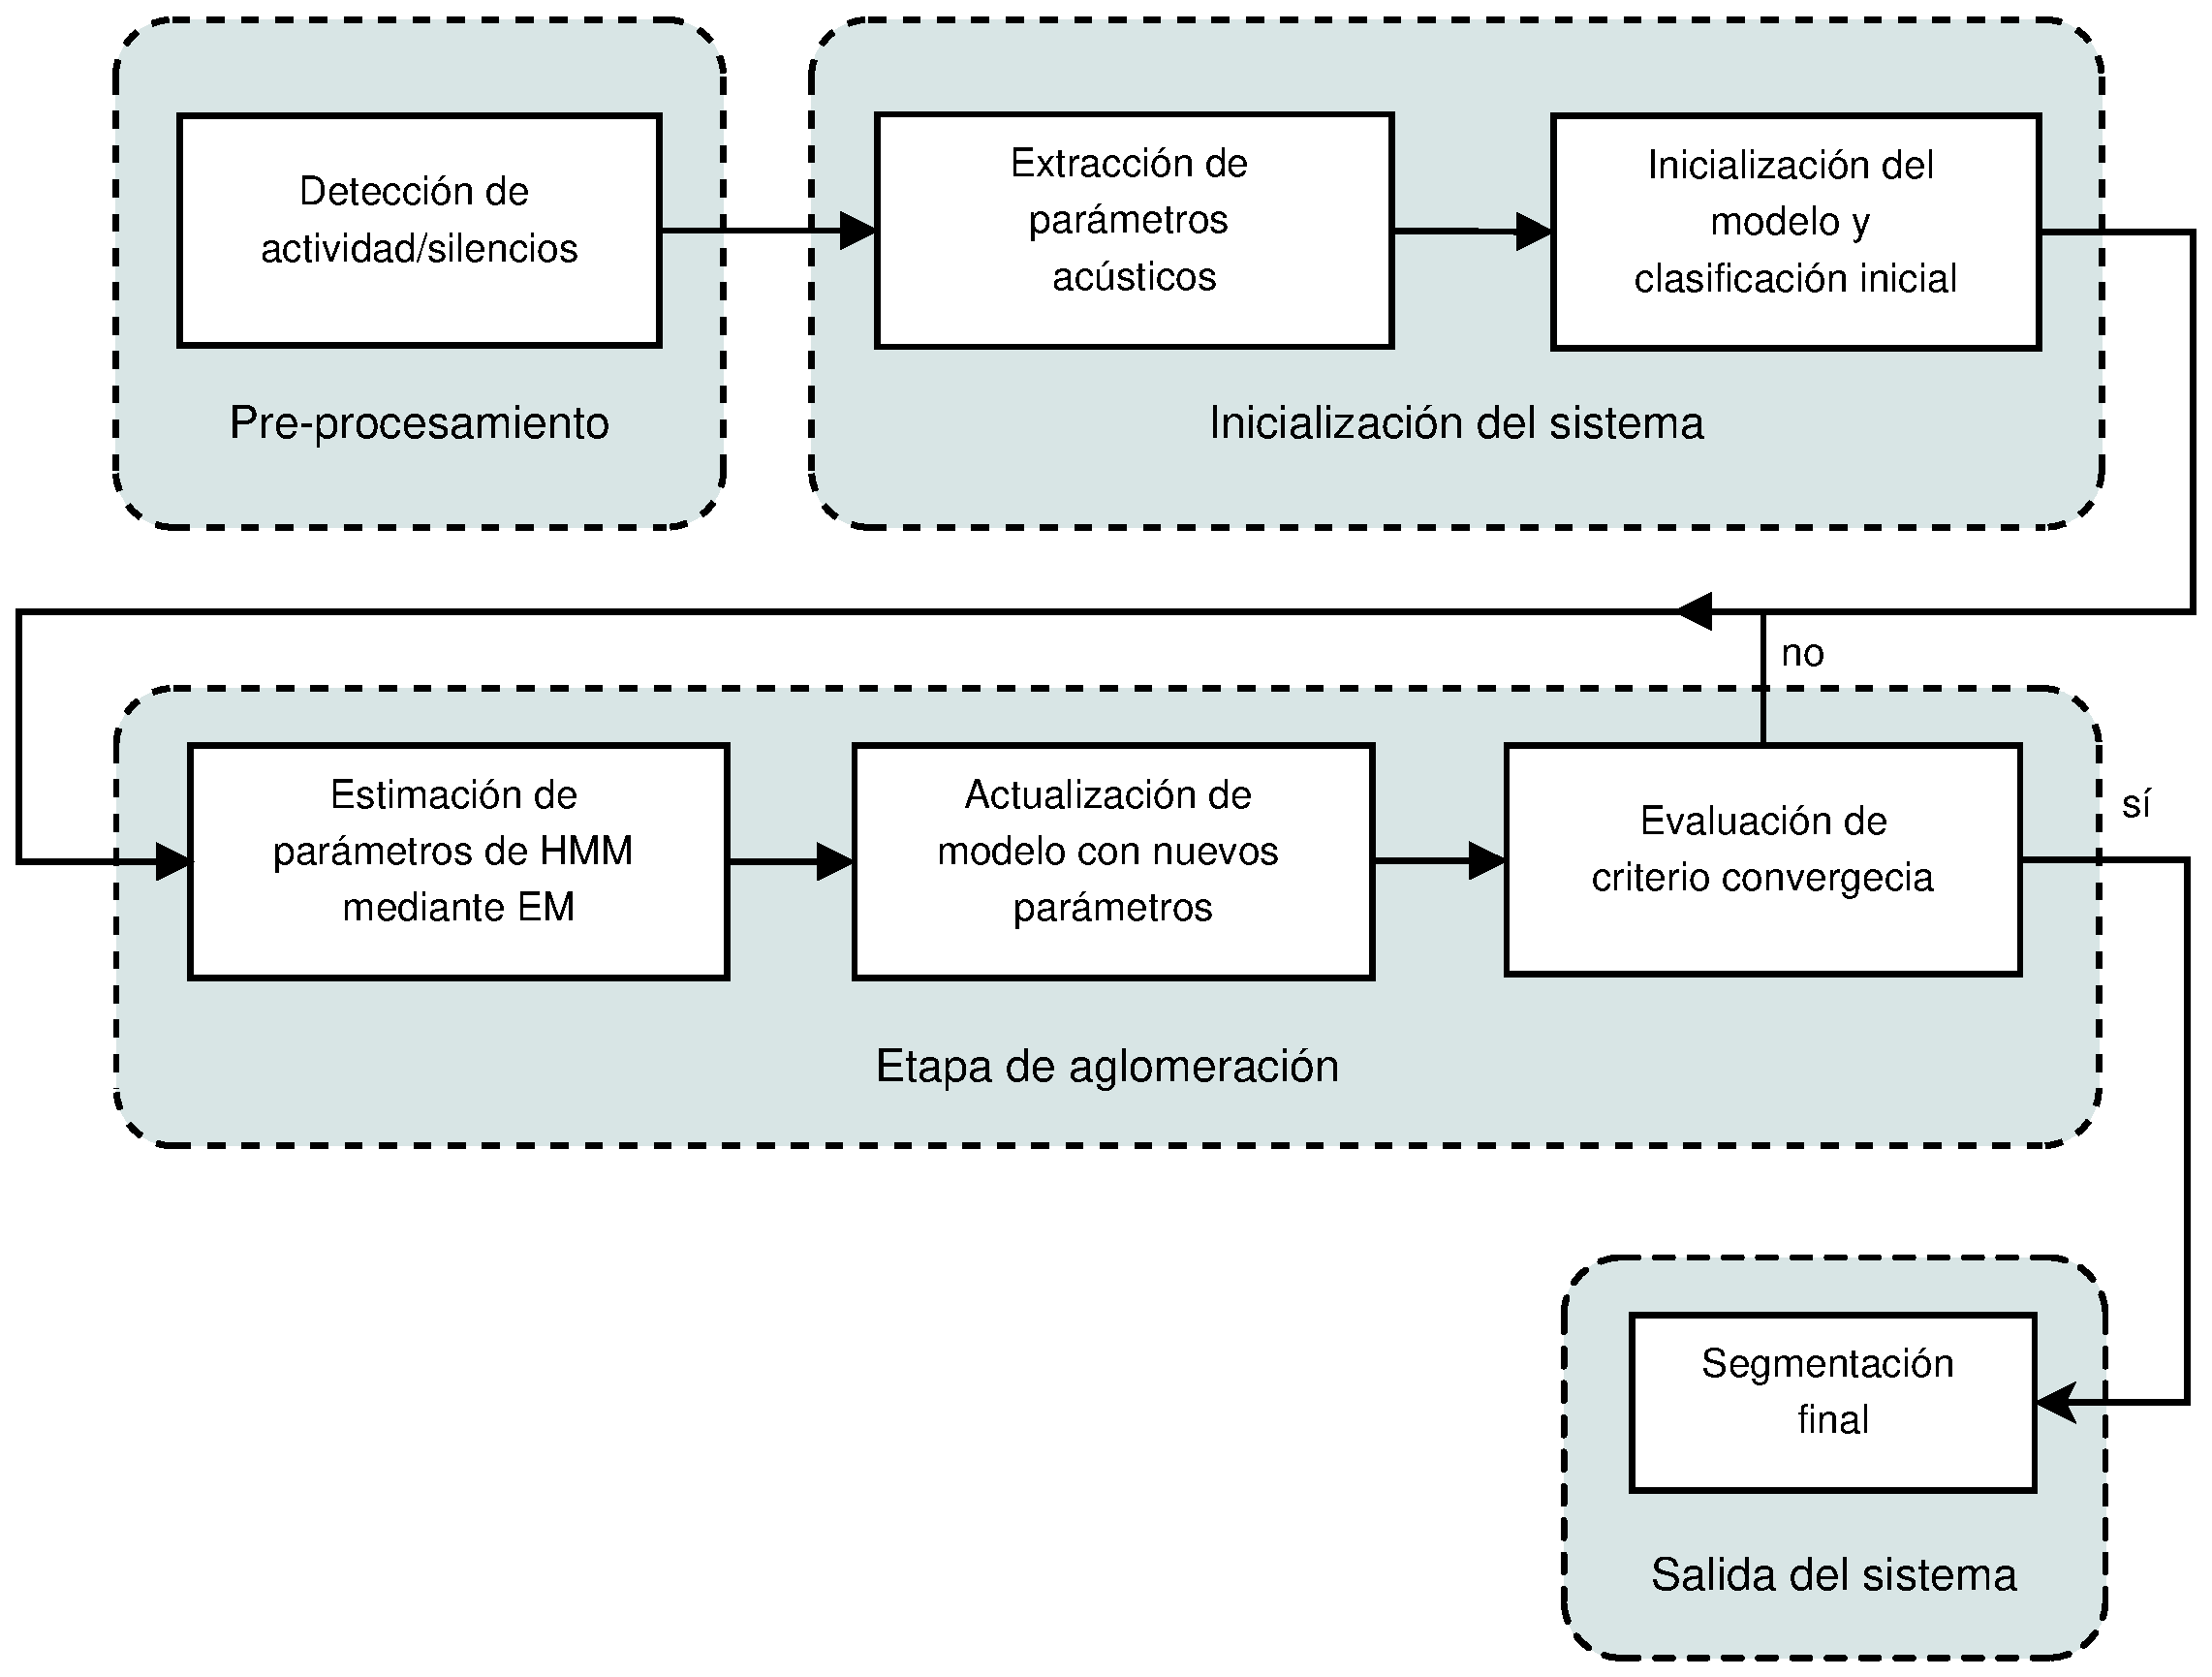
\includegraphics[width=1.4\linewidth]{gfx/chap2/ASR_flow}} \quad
  \caption[Esquema general del sistema.]{Esquema general del sistema. Se muestran las etapas principales para la estimación de la segmentación.}
  \label{fig:esquema}
\end{figure}


\section{Procesamiento acústico}

Antes de abordar de lleno el problema de \sd, se tiene que realizar cierto tratamiento a la señal de audio con la que se trabajará. 

Es decir, a partir de la señal de entrada (que se considerará es digital) se tratarán de obtener vectores de características cada cierto tiempo, que representen de forma adecuada los rasgos que nos interesan distinguir.

Una vez que se tienen estos vectores, se les aplica un algoritmo de aglomeración para entonces obtener un conjunto de etiquetas que se podrían considerar como posibles estados o palabras de diccionario referentes a la señal de audio.

El proceso en detalle se especifica a continuación: 

\subsection{Pre-procesamiento de señal de audio}

Se considera que se tiene una señal digital de voz, y que a partir de ésta se identificarán a las diferentes personas que hablan durante la grabación.

\begin{figure}[ht]
  {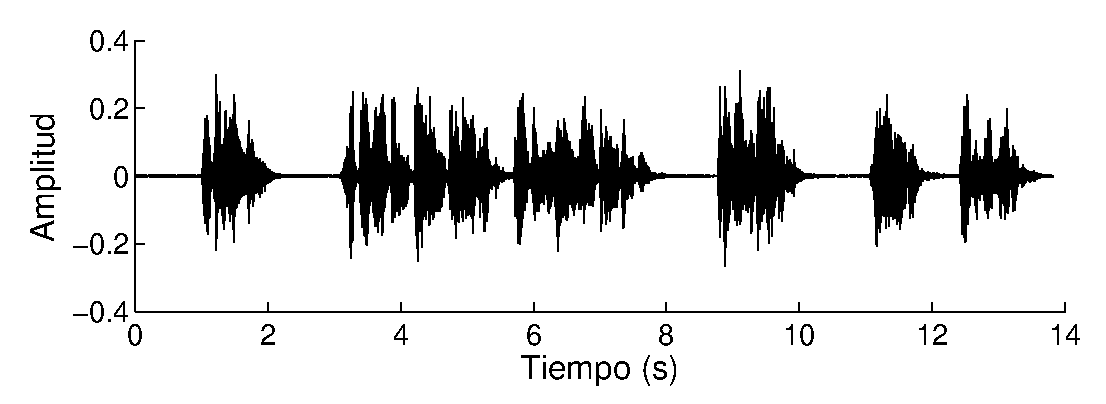
\includegraphics[width=0.9\linewidth]{gfx/chap2/signal0}} \quad
  \caption{Señal original de audio.}
  \label{fig:sign_orig}
\end{figure}

El primer paso en el procesamiento de la señal, es tanto la detección como eliminación de silencios; pues éstos realmente no nos interesan para la modelación del sistema. A esta etapa de pre-procesamiento se le suele conocer como \ac{SAD}.

\graffito{Nota: Tanto en ancho de la ventana, como el umbral del \ac{SAD} se pueden ajustar dependiendo de las características de la señal.}

Para realizar entonces la detección de los silencios, en esta primer etapa y como un primer intento para la eliminación de silencios, se hace una detección básica de qué partes de la señal son mayormente silencios.

Para ésto, se utiliza una ventana móvil que se irá recorriendo a lo largo señal, y que irá calculando el total de energía de la señal dentro de la ventana. Se considerará entonces silencio aquellas partes de la señal cuyo amplitud total esté debajo de un umbral específico.

A partir de esta ventana se podrán diferencias las partes que se tratarán como silencio de las partes que serán la señal resultante.

Como ya se mencionó, esta es una forma sencilla aunque no muy robusta de detectar en qué partes de la señal hay actividad. En otros trabajos, como 
en el de Istrate~et~al.~\cite{Istrate2005}, se presenta una etapa de \ac{SAD} mucho más profunda y diseñada para funcionar en entornos con múltiples micrófonos y proponen entrenar un modelo \ac{GMM} que sirva como clasificador luego para los silencios; que si bien muestra varias ventajas, está fuera del alcance de este trabajo.

\begin{figure}[ht]
  \begin{subfigure}[b]{\textwidth}
    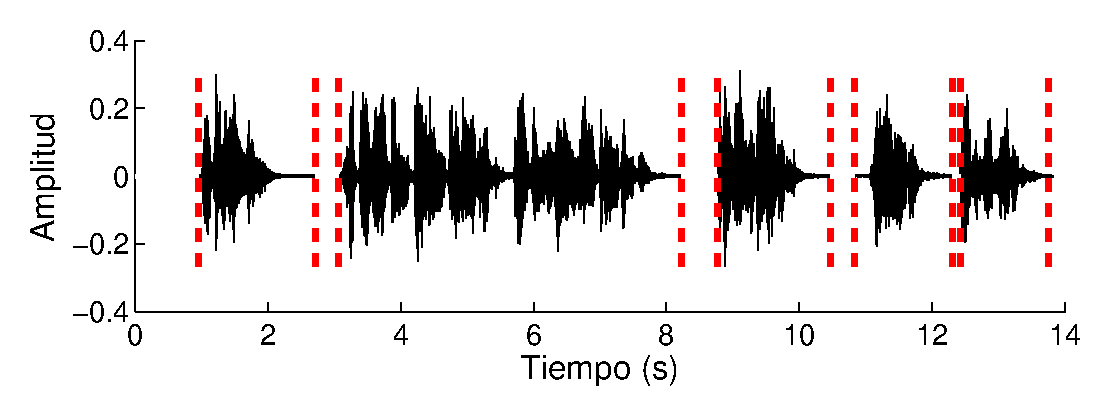
\includegraphics[width=0.9\linewidth]{gfx/chap2/signal1}
    \caption{Señal original con silencio identificado.}
    \label{fig:sign_silence}  
  \end{subfigure}

  \begin{subfigure}[b]{\textwidth}
    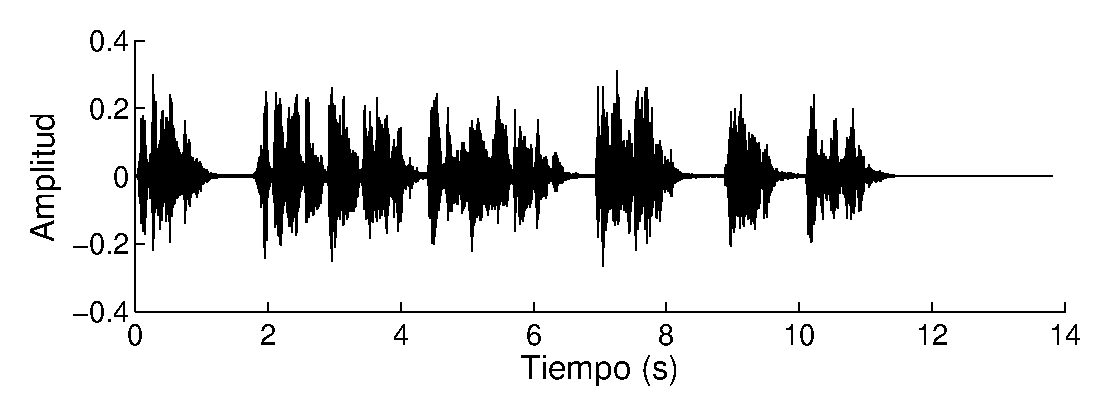
\includegraphics[width=0.9\linewidth]{gfx/chap2/signal2}
    \caption{Señal procesada y recortada.}
    \label{fig:sign_trunc}  
  \end{subfigure}
  
  \caption[Identificación/eliminación de silencios.]{Identificación y eliminación de silencio en señal.}  
  \label{fig:sign_ident}  
\end{figure}

Como se observa en la \autoref{fig:sign_trunc} basta entonces con eliminar los segmentos que contienen baja energía y reagrupar los segmentos restantes.

Con esto, se obtiene una señal en general más pequeña, y que se podría  considerar sólo contiene realmente los datos que se desea modelar.

\subsection{Obtención de características acústicas}

Una vez que se tiene la señal ya sin silencios, se trata de buscar características propias de la señal de audio que nos permitan identificar de buena forma los cambios de voz a través de la señal.

Tanto la extracción como selección de la mejor representación paramétrica de la señal de audio es una importante tarea en el diseño de cualquier sistema relacionado al reconocimiento o procesamiento de señales de audio. 

Para la tarea de \sd, se usarán los \ac{MFCC}, que son ampliamente utilizados por ejemplo en \sd~ entre otros procesos relacionados al procesamiento de voz; cuyo objetivo es comprimir la señal de audio eliminando la información que no es útil para análisis fonético.

Cabe mencionar, que originalmente los \ac{MFCC} fueron utilizados para la tarea específica de reconocimiento de voz por Davis~y~Mermelstein~\cite{Davis1980}, por lo que al momento de diseñarlos se trataba principalmente de que palabras iguales fueran parametrizadas de la misma manera sin importar quién la pronunciara. 

Esto va en contra del proceso requerido en \sd, puesto que se desea identificar a las diferentes personas que hablan, sin dar tanta importancia a qué es lo que están diciendo; por lo que la tarea de segmentación de señales de audio se vuelve un poco más complicada.

Para calcular los \ac{MFCC}, se usa la Escala de Frecuencia Mel, que está espaciada de forma lineal en frecuencias bajas, mientras que aumenta su separación de forma logarítmica para frecuencias más altas. Este cambio de separación se realiza comúnmente a partir de los $1000Hz$. 

A partir de esta escala, se diseña un banco de filtros triangulares que después se usará para construir un espectrograma de la señal (Ver \autoref{fig:sign_melfb}). Puesto que el banco de filtros de Mel trabajan en la frecuencia; a la señal de audio se le calcula la \ac{FT} y entonces a ésta es a quien se le aplica el banco de filtros.

\begin{figure}[t]
  \myfloatalign
  {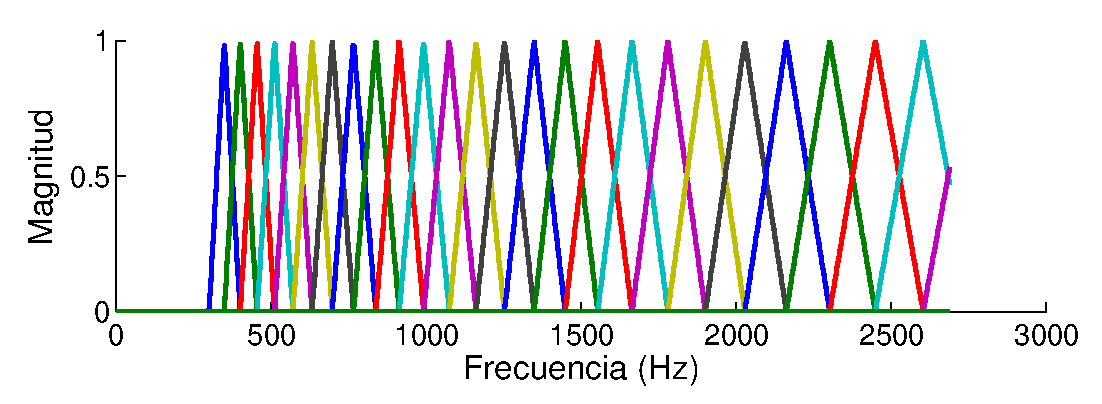
\includegraphics[width=0.9\linewidth]{gfx/chap2/mfcc_filterbank}} \quad
  \caption{Banco de filtros triangulares en frecuencia Mel.}
  \label{fig:sign_melfb}
\end{figure}  

Sea pues \autoref{fig:sign_trunc} la señal procesada sin los silencios, la respuesta que se obtiene al aplicar la \ac{FFT} y luego el banco de filtros de \autoref{fig:sign_melfb} se puede observar en la figura \autoref{fig:sign_melres}.

Para ser más específicos, la operación que se utiliza para construir el espectrograma es en realidad la \ac{STFT}; que si bien está basada en una \ac{FT}, se aplica de forma separada a segmentos de la señal de audio. 

Se puede pensar como una secuencia de operaciones \ac{DCT} por segmentos usando una ventana movible. Como menciona Rabiner~y~Schafer~\cite{Rabiner2007}, este método es la base en la mayoría de las técnicas relativas a procesamiento de voz, pues la construcción de un espectrógrama permite de forma sencilla analizad (y visualizar) la respuesta de una señal a un cierto banco de filtros entonado a alguna frecuencia.

Esto permite definir una resolución específica con la que se trabajará, dependiendo de las características que se desean obtener. Por ejemplo, si se desea que la respuesta tenga una mejor resolución en frecuencia, se debería usar un tamaño de ventana mayor, en relación a la periodicidad de la señal; aunque esto implicará que se pierda sensibilidad en la dimensión del tiempo. Por otro lado, si se utiliza una ventana de tamaño menor, la respuesta será mucho más precisa en cuanto al tiempo, pero se la resolución en frecuencia será más burda \cite{Rabiner1993}.

\begin{figure}[t]
  \myfloatalign
  {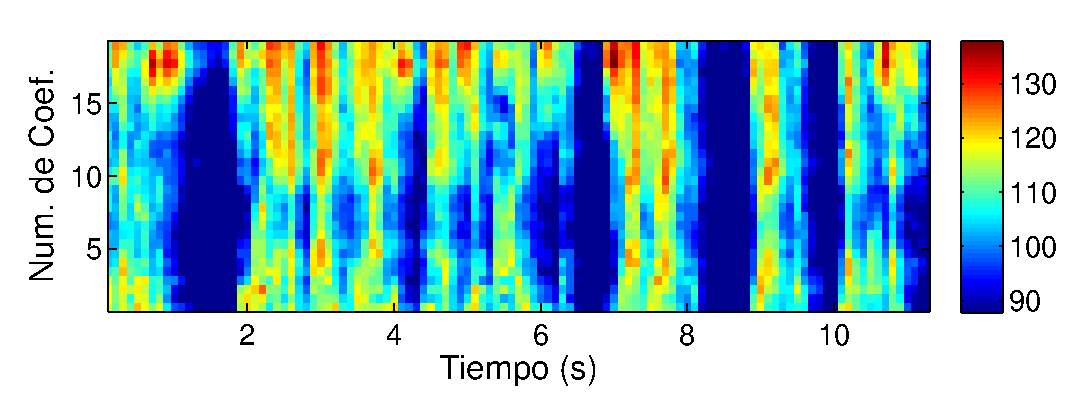
\includegraphics[width=0.9\linewidth]{gfx/chap2/mfcc_result2}} \quad
  \caption{Respuesta al banco de filtros.}
  \label{fig:sign_melres}
\end{figure}

La matriz que se muestra en \autoref{fig:sign_melres} corresponde a la respuesta al banco de filtros. Cada renglón representa la frecuencia a la que está entonado un filtro en específico del banco; mientras que cada columna indica la muestra en tiempo en que se analiza la señal. Por último, la intensidad en la escala de colores es la respuesta al banco de filtros, o la amplitud con la que cada frecuencia se presenta en cierto momento.

La dimensión de esta matriz dependerá de la misma construcción del banco de filtros (tanto el número de canales que se usarán, como el tamaño de ventana que se usará para las convoluciones); pero en general se obtendrán matriz de gran tamaño; por lo que es conveniente tratar de disminuir la dimensionalidad de estos datos.

Para esto, a la respuesta obtenida del banco de filtros se le aplicará la \ac{DCT}, para tratar de concentrar la energía en ciertos componentes (los primeros $n$ coeficientes), y descartar los restantes. A esta etapa se le conoce como extracción de los coeficientes cepstrales. 

\begin{algorithm}[bt]
   \caption{\textit{MFCC}}
   \label{alg:mfcc}
\begin{algorithmic}
   \STATE {\bfseries Input:} \\ Señal digital $\lbrace s_n \rbrace_1^T $,
   \STATE Iniciar $\mu_{1:k} = sample(x_{1:N}, K)$   
   
   \STATE $t = 0$
   \STATE $l_{1:N}^{(t)} = 0$
      
   \REPEAT  
   \STATE $t=t+1$ 
   \STATE $l_n^{(t)} = \text{arg min}_k {\left \| x_n - \mu_k \right \|}^2 $
   \STATE $r_{nk}$ = $\mathbbm{1}_k\left(l_n^{(t)}\right)$
   \STATE $\mu_k = \left\lbrace {\sum_{n=1}^N r_{nk} x_n} \right\rbrace / \left\lbrace {\sum_{n=1}^N r_{nk}} \right\rbrace $
   \UNTIL{$l^{(t)}$ == $l^{(t+1)}$}
\end{algorithmic}
\end{algorithm}

Como ya se mencionó previamente, el banco de filtros utilizado está separado  en la frecuencia Mel, pues aproximan mucho mejor la respuesta del sistema auditivo humano que un banco de filtros linealmente espaciados \cite{Vyas2013}. 

Después de este proceso, nuestros datos se podrían representar de la siguiente manera (\autoref{fig:sign_mfcc}) que son los \ac{MFCC} que antes habíamos mencionado.
\begin{figure}[t]
  \myfloatalign
  {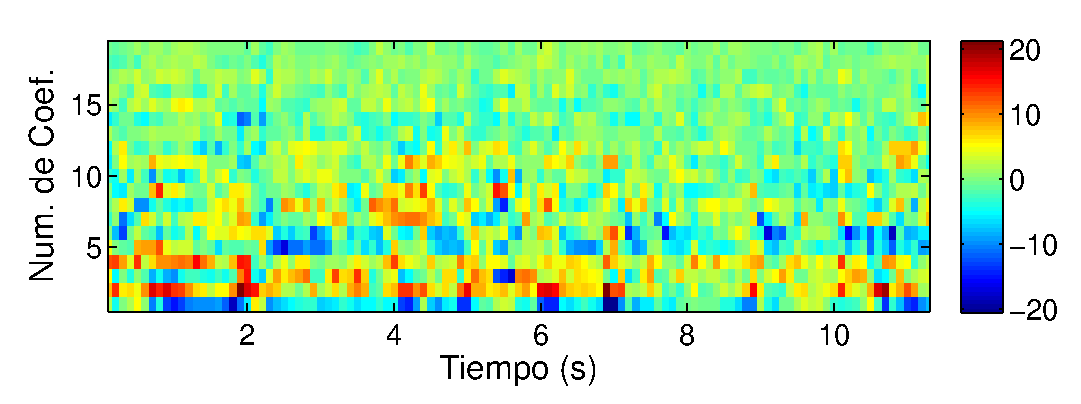
\includegraphics[width=0.9\linewidth]{gfx/chap2/mfcc_result3}} \quad
  \caption{Mel Frequency Cepstrum Coefficients.}
  \label{fig:sign_mfcc}
\end{figure}

Por último, para los modelos que usaremos, se necesitan que las características estén de cierta forma \textit{discretizadas}, es decir, no nos es útil el tener para cada observación en el tiempo un vector de características; sino que necesitamos una etiqueta o clase para cada observación. 

Para esto, podemos utilizar diferentes métodos tanto de reducción de dimensionalidad como de agrupación/clasificación. Como primer idea, utilizaremos el método de \textit{k-means} para agrupar los vectores de acuerdo a su cercanía en el espacio euclidiano.

Se tendría entonces el siguiente resultado para nuestra matriz de MFCC obtenida:
\begin{figure}[t]
  \myfloatalign
  {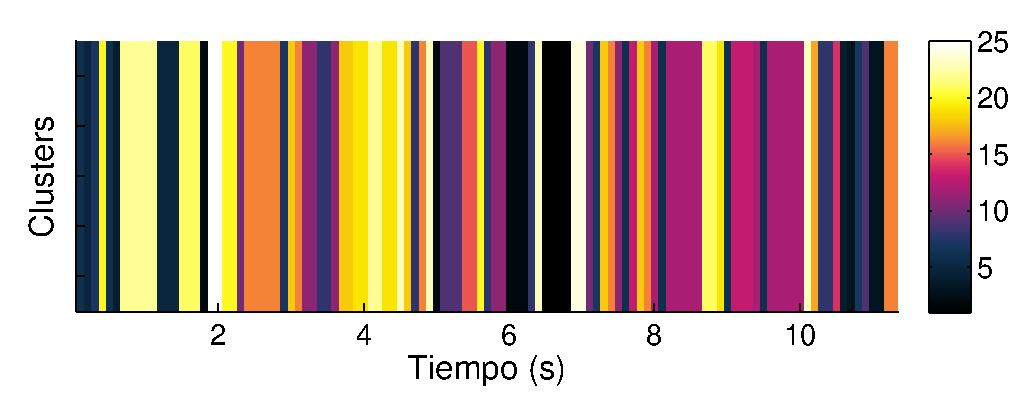
\includegraphics[width=0.9\linewidth]{gfx/chap2/mfcc_result4}} \quad
  \caption{MFCC agrupados con k-means++.}
  \label{fig:sign_clusters}
\end{figure}
Cabe aclarar que usamos una variante del algoritmo original de k-means, que se llama \textit{k-means++} \cite{Arthur2007} y que propone una mejor inicialización para que el algoritmo converja más rápido. En \autoref{alg:kmeanspp} se describe mejor esta etapa inicial.

\begin{algorithm}[bt]
   \caption{\textit{k-means}}
   \label{alg:kmeans}
\begin{algorithmic}
   \STATE {\bfseries Input:} \\ Conjunto de datos $\lbrace x_n \rbrace_1^N $, número de grupos $K$
   \STATE 
   \STATE Iniciar $\mu_{1:k} = sample(x_{1:N}, K)$   
   
   \STATE $t = 0$
   \STATE $l_{1:N}^{(t)} = 0$
      
   \REPEAT  
   \STATE $t=t+1$ 
   \STATE $l_n^{(t)} = \text{arg min}_k {\left \| x_n - \mu_k \right \|}^2 $
   \STATE $r_{nk}$ = $\mathbbm{1}_k\left(l_n^{(t)}\right)$
   \STATE $\mu_k = \left\lbrace {\sum_{n=1}^N r_{nk} x_n} \right\rbrace / \left\lbrace {\sum_{n=1}^N r_{nk}} \right\rbrace $
   \UNTIL{$l^{(t)}$ == $l^{(t+1)}$}
\end{algorithmic}
\end{algorithm}

\begin{algorithm}[bt]
   \caption{\textit{k-means++}}
   \label{alg:kmeanspp}
\begin{algorithmic}
   \STATE {\bfseries Input:} \\ Conjunto de datos $\lbrace x_n \rbrace_1^N $, número de grupos $K$
   \STATE 
   \STATE $\mu_{1} = sample(x_{1:N}, 1)$   
   \FOR{k:=2 \TO $K$} 
     \STATE $m_n = \text{arg min}_{\mu_j} {\left \| x_n - \mu_j \right \|}^2 
      ~~\forall~~ j = {1, ..., k-1}; ~n = {1, ..., N} $
     \STATE $D_{n} = dist(x_n, m_n) ~~\forall~~  n = {1, ..., N}$
     \STATE $p_{n} = D_{n}^2 ~~\forall~~  n = {1, ..., N}$
     \STATE $\mu_{k} = sample(x_{1:N}, 1, p_{1:N})$   
   \ENDFOR
   
   \STATE $t = 0$
   \STATE $l_{1:N}^{(t)} = 0$
      
   \REPEAT  
   \STATE $t=t+1$ 
   \STATE $l_n^{(t)} = \text{arg min}_k {\left \| x_n - \mu_k \right \|}^2$
   \STATE $r_{nk}$ = $\mathbbm{1}_k\left(l_n^{(t)}\right)$
   \STATE $\mu_k = \left\lbrace {\sum_{n=1}^N r_{nk} x_n} \right\rbrace / \left\lbrace {\sum_{n=1}^N r_{nk}} \right\rbrace $
   \UNTIL{$l^{(t)}$ == $l^{(t+1)}$}
\end{algorithmic}
\end{algorithm}

Ahora sí, con nuestro vector de etiquetas correspondiente a la señal de audio, se podrá aplicar un modelo y tratar de inferir los parámetros que le correspondan.


% section section_name (end)

\begingroup
  \let\clearpage\relax
  %!TEX root = ../Thesis.tex

%*****************************************
\chapter{Modelos de Márkov}\label{ch:chap3}
%*****************************************

\epigraphhead[70]{
\epigraph{Essentially, all models are wrong, but some are useful.}
         {George E. P. Box}}

Como ya se mencionó en el \autoref{ch:chap2}, se debe proponer un modelo acústico o generativo, que será la forma en que entenderemos y trataremos de abstraer la conversación o diálogo, de acuerdo a las características que nos interesan recuperar.

Puesto que lo que nos interesa principalmente es identificar a las diferentes personas que participan en una conversación, nuestro modelo se deberá parametrizar de forma que logre capturar las características esenciales en la conversación; así como no tomar en cuenta información que no nos sea de utilidad para esta tarea, como por ejemplo, qué es lo que se está diciendo.

En aprendizaje máquina, por modelo generativo se entiende un modelo probabilístico para generar datos aleatoriamente que correspondan a la naturaleza de un cierto conjunto de datos que tengamos.

Al proponer un modelo generativo, se busca representar y de forma concisa poder parametrizar un fenómeno o situación de la que se obtuvieron los datos.
Cuando los datos son secuenciales, se suelen agrupar en dos tipos, de acuerdo a las características de la distribución que los generó: distribuciones estacionarias y distribuciones no estacionarias.

En el caso de secuencias de datos estacionarias, se considera que los datos \textit{evolucionan} a través del tiempo, pero la distribución a partir de la cuál fueron generados permanece igual; mientras que para el caso de datos no estacionarios, su distribución generativa varía también según pasa el tiempo.

Para el problema de \sd, consideraremos que los datos son estacionarios; es decir, supondremos que su distribución generativa no cambia. Para resolver nuestro problema entonces trataremos a partir de los datos ajustar una distribución inicial e inferir sus parámetros correspondientes.

Este tipo de abstracción, permiten modelar una gran cantidad de situaciones, en las que se tienen observaciones de acuerdo al tiempo y se quiere predecir el siguiente valor en la serie, dadas la observaciones que se tienen hasta el momento.

Comúnmente se suelen considerar únicamente las observaciones más recientes, pues son las que pudiéramos pensar son más informativas para la predicción; además de que al asumir que las predicciones de nuevos datos sólo dependen de las últimas observaciones, nos permite simplificar mucho el modelo de la distribución generativa.

Para trabajar con este tipo de datos, se puede usar entonces un modelo de Márkov que es un proceso aleatorio muy trabajado en la teoría de probabilidad, que incorpora una cantidad mínima de memoria, sin necesariamente llegar a ser un proceso sin memoria.

Se puede pensar como una red bayesiana en la que se asume la independencia de las variables aleatorias que corresponden a las predicciones futuras con todas las observaciones excepto las últimas (i.e. el futuro es independiente del pasado, dado el presente).

\section{Cadena de Márkov}

\graffito{Se entiende por v.a. i.i.d aquellas que son independientes entre sí y que fueron muestreadas de la misma distribución}

El modelo generativo más sencillo que se podría pensar, es considerar que todas las observaciones son variables aleatorias independientes e idénticas distribuidas (v.a. i.i.d) cuyo modelo gráfico se muestra en la \autoref{fig:mod_iid}.

\begin{figure}[tp]
        \myfloatalign
        {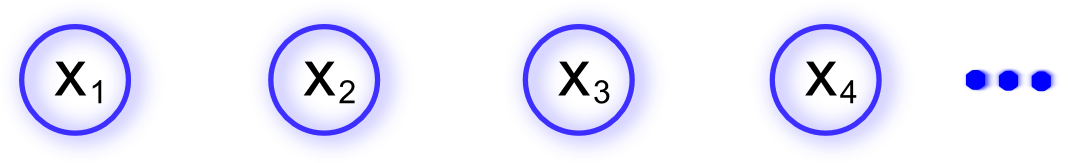
\includegraphics[width=0.6\linewidth]{gfx/chap3/mod-iid}}        
        \caption{Observaciones independientes e idénticamente distribuidas.}
        \label{fig:mod_iid}
\end{figure}

Al asumir que no hay ninguna dependencia entre los datos, sin embargo, se pierde la información relativa al orden en que se fueron dando estas observaciones; situación que en muchos casos nos interesa conservar.

Si se tiene un conjunto $N$ de observaciones $\mb{X} = \lbrace x_1, ..., x_N \rbrace$, y se asume que son i.i.d, la distribución conjunta de la secuencia de datos se puede escribir como sigue:
\begin{equation}
\label{eqn:2-1}
p(x_1, ..., x_N) ~=~ \prod_{n=1}^N p(x_n)
\end{equation}

En cambio, para expresar la dependencia entre un grupo de observaciones secuenciales, se puede utilizar un modelo probabilístico llamado \textit{modelo o cadena de Márkov}. Si por ejemplo, se considera que cada variable depende de todas las observaciones anteriores, entonces usando el teorema de Bayes
\graffito{Del teorema de Bayes se tiene la siguiente expresión
$${P(A \,|\, B) = \frac{P(B \,|\,A) P(A)}{P(B)}}$$ } 
se puede escribir la distribución conjunta de las observaciones de la siguiente manera:
\begin{equation}
\label{eqn:2-2}
p(x_1, ..., x_N) ~=~ \prod_{n=1}^N p(x_n \,|\, x_1, ..., x_{n-1}).
\end{equation}

Ahora, si se asume que cada $x_n$ es independiente de las observaciones anteriores excepto de la observación anterior $x_{n-1}$, se tiene que la distribución conjunta se puede escribir de forma más sencilla utilizando el teorema de separación D \footnote{Ver anexo}, puesto que 
\begin{equation}
\label{eqn:2-3}
p(x_n \,|\, x_1, ..., x_{n-1}) ~=~ p(x_n \,|\, x_{n-1})
\end{equation}

A este modelo probabilístico se le conoce como cadena de Márkov de primer orden y la probabilidad conjunta de las observaciones está dada por:
\begin{equation}
\label{eqn:2-4}
p(x_1, ..., x_N) ~=~ p(x_1) \prod_{n=2}^N p(x_n \,|\, x_{n-1}).
\end{equation}
mientras que su modelo gráfico corresponde a la \autoref{fig:mod_mm1}
\begin{figure}[tp]
        \myfloatalign
        {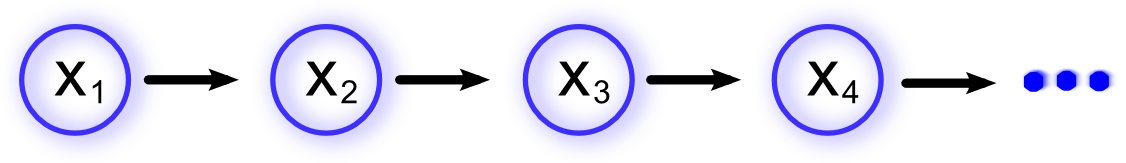
\includegraphics[width=0.6\linewidth]{gfx/chap3/mod-mm1}}
        \caption{Modelo de Márkov de primer orden.}
        \label{fig:mod_mm1}
\end{figure}

Aunque el modelo es mucho más general, puede que se necesite representar de forma más fuerte la dependencia con las observaciones anteriores, por lo que se pueden usar cadenas de Márkov de órdenes superiores.

Al caso en el que $x_n$ dependa de las dos observaciones previas se le conoce como cadena de Márkov de segundo orden; y siguiendo el mismo proceso, la distribución conjunta de las observaciones se puede escribir como 
\begin{equation}
\label{eqn:2-5}
p(x_1, ..., x_N) ~=~ p(x_1) \cdot p(x_2 \,|\, x_1) 
        \prod_{n=3}^N p(x_n \,|\, x_{n-1}, x_{n-2})
\end{equation}
puesto que se tiene que $x_n \perp x_1, ..., x_{n-3} \,|\, x_{n-1}, x_{n-2}$.

En este caso su modelo gráfico correspondiente es la \autoref{fig:mod_mm2}, en el que se puede observar la dependencia de una $x_n$ en específico únicamente con sus dos observaciones anteriores.

\begin{figure}[tp]
        \myfloatalign
        {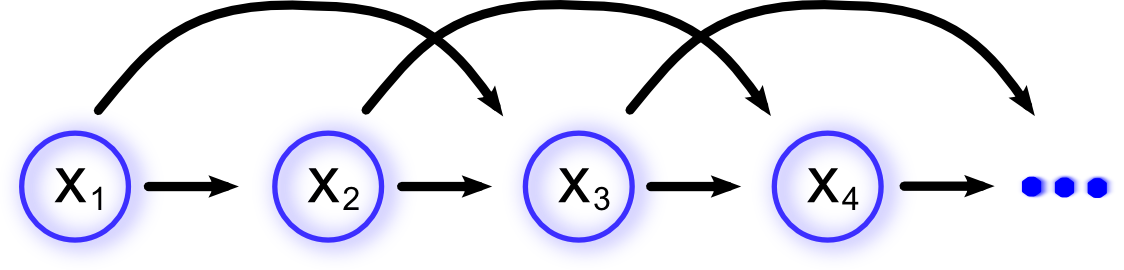
\includegraphics[width=0.6\linewidth]{gfx/chap3/mod-mm2}}
        \caption{Modelo de Márkov de segundo orden.}
        \label{fig:mod_mm2}
\end{figure}

Se puede generalizar entonces para cualquier $M$ un modelo de Márkov de $M$-ésimo orden, aunque al considerar demasiados estados previos se puede complicar de más el modelo; pues el número de parámetros implicados aumenta de forma exponencial al orden del modelo de Márkov.

Para evitar que el modelo se vuelva demasiado complejo, así como para no hacer alguna suposición a priori sobre cuál es el orden es del modelo generativo, se puede introducir una variable oculta, que permita cambiar el planteamiento del modelo. 

Se considera entonces una variable latente $z_n$ correspondiente a cada  observación $x_n$, y entonces el conjunto de variables latentes forman una cadena de Márkov, como se muestra en la \autoref{fig:mod_hmm1}.

Se asumirá entonces 
\begin{equation}
\label{eqn:2-6}
z_{n+1} \perp z_{n-1} \,|\, z_{n}
\end{equation}

Y entonces, usando la regla de la cadena, la distribución conjunta para este modelo es la siguiente: 
\begin{equation}
\label{eqn:2-7}
p(x_1, ..., x_N, z_1, ..., z_N) ~=~ 
        p(z_1) \left [ \prod_{n=2}^N p(z_n \,|\, z_{n-1}) \right ] 
\prod_{n=1}^N p(x_n \,|\, z_{n}).
\end{equation}

\begin{figure}[tp]
        \myfloatalign
        {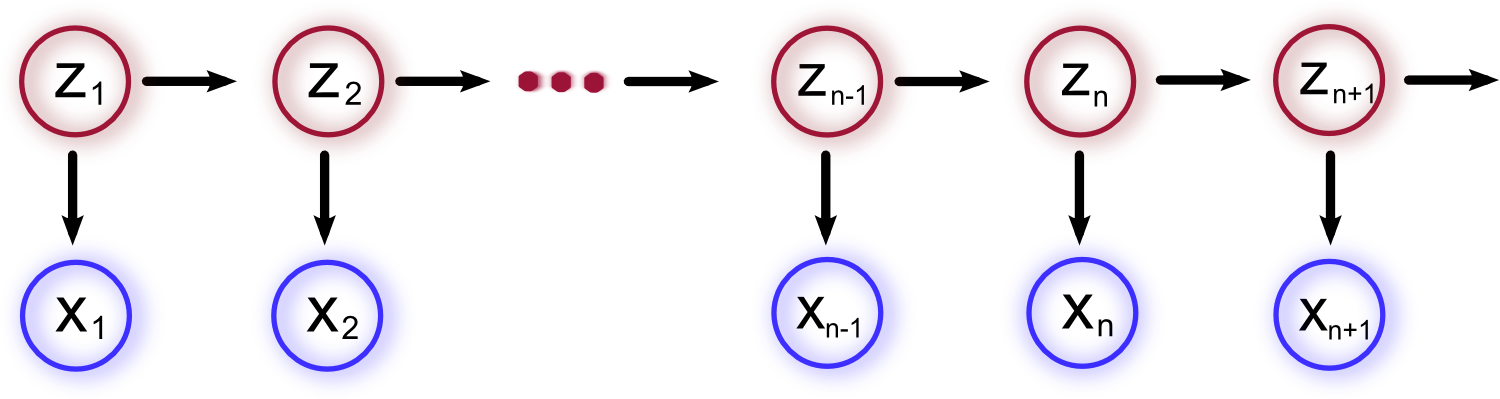
\includegraphics[width=0.8\linewidth]{gfx/chap3/mod-hmm1}}
        \caption{Modelo oculto de Márkov.}
        \label{fig:mod_hmm1}
\end{figure}

Para éste último modelo gráfico, si las variables latentes son discretas, entonces se le conoce como \acf{HMM}, y es justo el modelo que se utilizará para resolver la tarea de \sd.

\section{Cadena oculta de Márkov}

Un \acl{HMM}, sigue siendo entonces un modelo para datos secuenciales, en los que además se introduce el concepto de una variable oculta de la cual dependen las observaciones que se tienen; y de forma más especifica, esta variable oculta es discreta. 

Usando un \ac{HMM} entonces podemos modelar un proceso bivariado discreto en el tiempo, con ciertas propiedades interesantes que se mencionarán más adelante.

Nuestro modelo \ac{HMM}, se puede pensar como una mezcla de distribuciones en la que la densidad tiene un distribución dada por $p(x|z)$, es decir, la mezcla de los componentes está dada por las observaciones previas.

Se puede considerar entonces, que cada variable latente $z_n$ tendrá una distribución multinomial discreta, que indicará cuál componente de la mezcla de distribuciones es la que ha generado la observación $x_n$. Para ésto, se usará la notación \unk, que corresponde a un conjunto de variables indicador $z_{nk} \in \lbrace 0, 1 \rbrace$, donde $k = 1, ..., K$ señalando cuál de las $K$ distribuciones generó a la variable $x_n$, \ie, si el componente generador de $x_n$ fue la $k$-ésima mezcla, entonces $z_{nk} = 1$ y $z_{nj} = 0$ para todo $j \neq k$.

Ahora, se tiene que cada variable $z_n$ depende únicamente de $z_{n-1}$, y puesto que las variables latente son vectores binarios de $K$ dimensiones, entonces se tendría que la probabilidad condicional de $z_n \,|\, z_{n-1}$ se puede representar mediante una tabla o matriz, que se denotará como $\mb{A}$, y será referida como \textit{matriz de probabilidades de transición}. 

Los componentes de la matriz de transición se definen tal que $A_{jk} \equiv p(z_{nk} = 1 \,|\,  z_{n-1, j} = 1)$, y puesto que son probabilidades, se cumple que $0 \leq A_{jk} \leq 1$ además de que $\sum_k A_{jk} = 1$. Considerando estas restricciones, entonces la matriz $\mb{A}$ tiene $K (K-1)$ parámetros independientes.

Se puede escribir entonces la probabilidad condicional de una variable latente $z_n$ dada la anterior variable latente $z_{n-1}$ de la siguiente forma: 
\begin{equation}
\label{eqn:2-8}
p(z_n \,|\, z_{n-1}, \mb{A}) = \prod_{k=1}^K \prod_{j=1}^K A_{jk}^{z_{n-1, j} 
        \cdot z_{nk}}
\end{equation}

Además, se tiene que considerar la variable latente inicial $z_1$, puesto que ésta no tiene una variable latente anterior, la \autoref{eqn:2-7} no aplica; por lo que entonces la probabilidad marginal de $z_1$ está representada por un vector de probabilidades $\pi$ tal que $\pi_k \equiv p(z_{1k})$, por lo que se puede reescribir como sigue: 
\begin{equation}
p(z_1 \,|\, \pi) = \prod_{k=1}^K \pi_k^{z_{1k}}
\label{eqn:2-9}
\end{equation}
y además se cumple que $\sum_k \pi_k = 1$ por definición.

La matriz de transición también se puede llegar a representar como un grafo dirigido, si se consideran las entradas de la matriz $\mb{A}$ como los pesos de las aristas, y los nodos son cada uno de los posibles $K$ estados. Por ejemplo, para el caso de una variable latente de $K = 3$ estados, se tendría el grafo de la \autoref{fig:mod_hmm2}.

\begin{figure}[tp]
        \myfloatalign
        {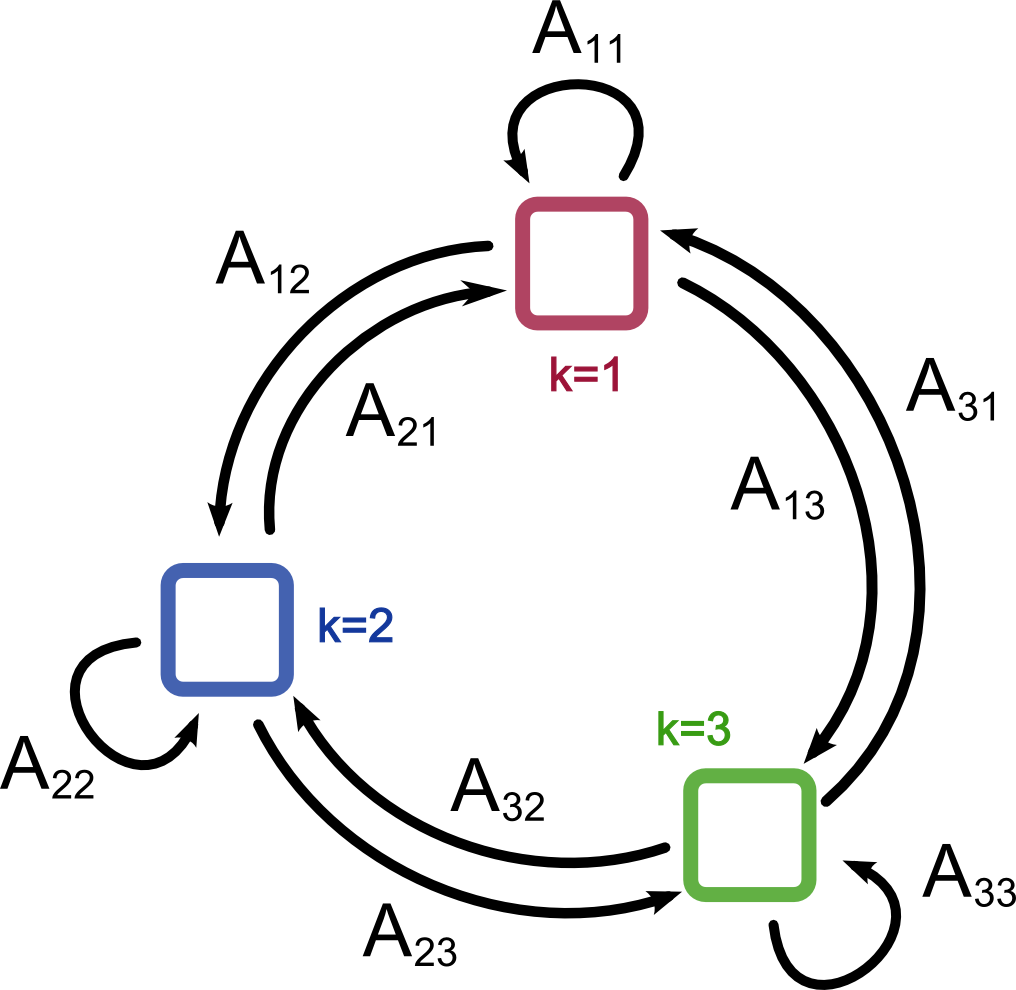
\includegraphics[width=0.4\linewidth]{gfx/chap3/mod-hmm2}}
        \caption{Matriz de transición de modelo oculto de Márkov (grafo).}
        \label{fig:mod_hmm2}
\end{figure}

De la misma manera, el grafo correspondiente a la matriz de transición, se puede representar como una rejilla a través del tiempo, en la que se mantienen los vértices y aristas del grafo, pero además se introduce la noción del tiempo. Como se observa en la \autoref{fig:mod_hmm3} 

\begin{figure}[tp]
        \myfloatalign
        {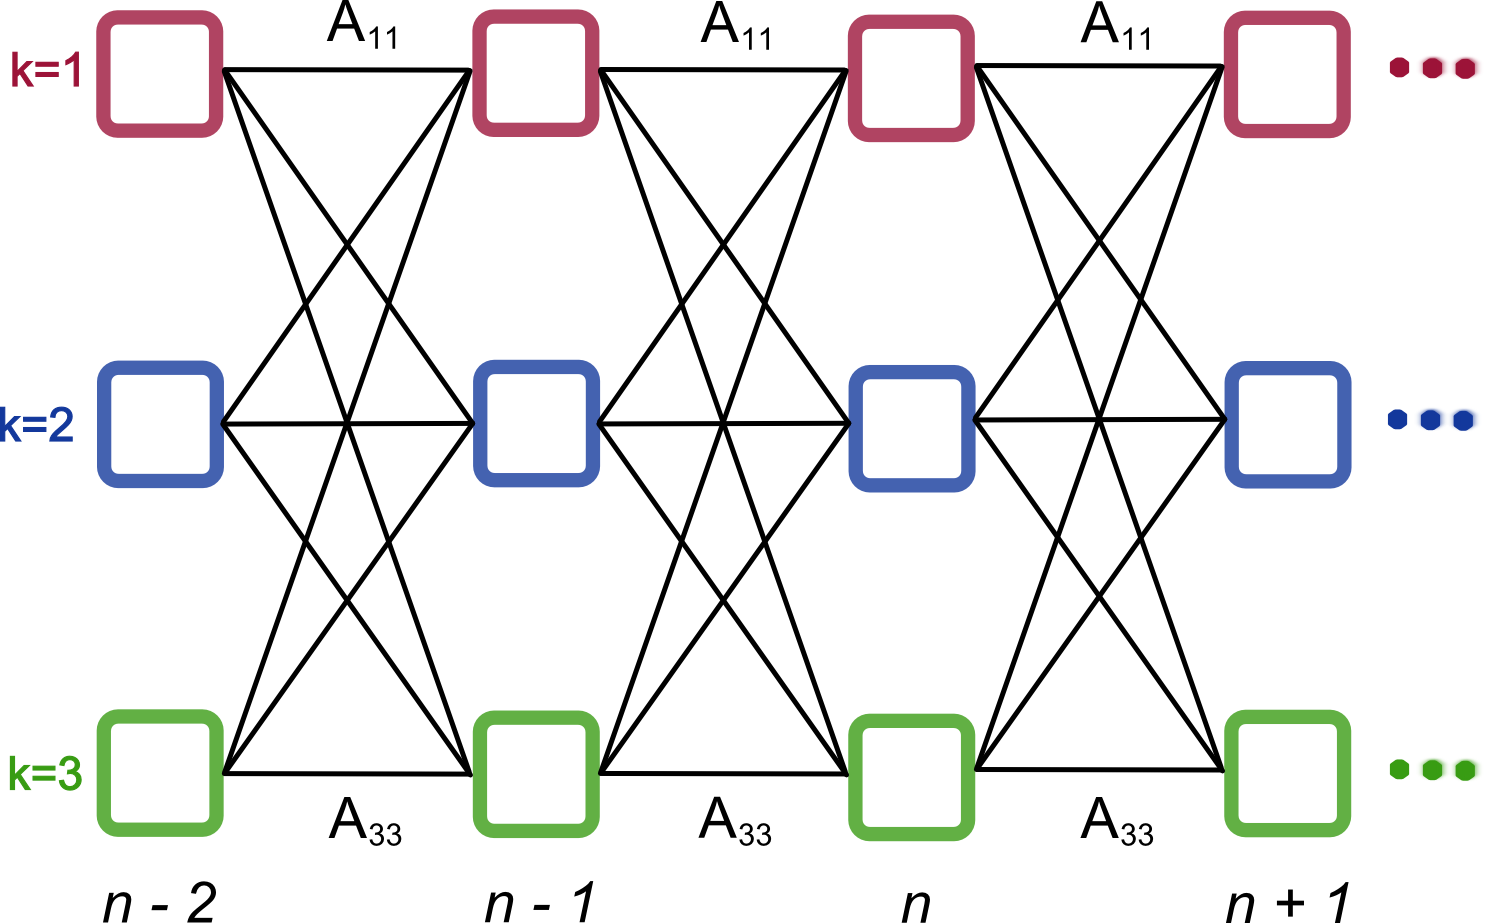
\includegraphics[width=0.63\linewidth]{gfx/chap3/mod-hmm3}}
        \caption{Matriz de transición de modelo oculto de Márkov (rejilla).}
        \label{fig:mod_hmm3}
\end{figure}

Por último, para completar el modelo se tiene que considerar además la distribución condicional de las variables observadas, es decir $p(x_n \,|\, z_n, \phi)$ donde $\phi$ es un conjunto de parámetros específicos a la distribución de $x$. Se les conoce como probabilidades de emisión, y puede ser tanto una distribución discreta como una continua. Para el caso en que la probabilidad de emisión esté dada por una distribución discreta, entonces se tendrá una tabla de probabilidades.

Para calcular entonces esta probabilidad de emisión, se tiene tanto $z_n$ como unos parámetros $\phi$ dados, por lo que entonces se tienen un vector de $K$ valores para cada uno de los posibles estados del vector indicador $z_n$.

Se puede escribir entonces la probabilidad de emisión como sigue:
\begin{equation}
p(x_n \,|\, z_n, \phi) = \prod_{k=1}^K p(x_n \,|\, \phi_k) ^ {z_{nk}}
\label{eqn:2-10}
\end{equation}
y entonces la probabilidad conjunta quedaría definida de la siguiente manera:
\begin{equation}
p(\mb{X}, \mb{Z} \,|\, \theta) 
= p(z_1 \,|\, \pi) \left[ \prod_{n=2}^N p(z_n \,|\, z_{n-1}, \mb{A}) \right]
        \prod_{n=1}^N p(x_n \,|\, z_n, \phi)
\label{eqn:2-11}
\end{equation}
donde $\mb{X} = \lbrace x_1, ..., x_N \rbrace$,~ $\mb{Z} = \lbrace z_1, ..., z_N \rbrace$~ y ~ $\theta = \lbrace \pi, \mb{A}, \phi \rbrace$ es el conjunto de parámetros requeridos por el modelo.

La intuición del modelo oculto de Márkov se puede entender más fácilmente si se revisa desde el punto de vista generativo. Primero, se muestrea la variable latente inicial $z_1$, de acuerdo a las probabilidades $\pi_k$, así como su correspondiente $x_1$. Luego, se debe escoger un $z_2$. Para esto, si se supone que $z_1$ es igual a algún estado $j$, entonces usando la matriz de transición se muestrea $z_2$ con probabilidades $A_{jk}$ para $k = 1, ..., K$, y de igual manera, su correspondiente variable observada $x_2$. Éste mismo proceso es el que se sigue para cada iteración en el tiempo, hasta que se forma completamente el modelo oculto de Márkov y se le conoce como \textit{muestreo ancestral} y se suele usar para modelos con grafos dirigidos.

Si la matriz de transición es predominantemente diagonal, entonces en la secuencia de datos puede que un mismo estado $i$ sea el que genere muchos puntos $x_n$, pues con poca probabilidad cambiará de un estado $i$ a $j$. Este fenómeno es justo el que se espera para el caso de \sd, pues usualmente una persona $p_i$ hablará durante mucho tiempo, y luego cuando otra persona $p_j$ toma la palabra, sucederá lo mismo.
  %!TEX root = ../Thesis.tex

%************************************************
\section{Estimación de Máxima Verosimilitud del HMM}
%************************************************

La tarea de aprendizaje de parámetros del \ac{HMM} se refiere a encontrar, dada una secuencia de datos observados, el mejor conjunto de probabilidades de transición y emisión.

Este problema es difícil de resolver, pues no se tiene una forma analítica de resolverlo \cite{Rabiner1989}. De hecho, dada una secuencia finita de observaciones como conjunto de entrenamiento, no hay forma óptima de estimar los parámetros verdaderos del modelo, y lo más que se puede hacer, es escoger $\theta = \left( \textbf{A}, \textbf{B}, \pi \right)$ tal que $P(\textbf{X} \,|\, \theta)$ corresponda a un máximo local usando algún algoritmo tipo \ac{EM} o técnicas de descenso de gradiente. 

A continuación, se presentará el algoritmo de Baum–Welch que es básicamente \ac{EM} aplicado a una cadena de Márkov, y que nos permitirá tanto inferir los parámetros $\theta$ del \ac{HMM} así como luego recuperar la secuencia de estados.

%\section{Estimación de parámetros del HMM}
\subsection{Estimación de parámetros del HMM}

Si se tiene un conjunto de datos observados $\mb{X} = \lbrace x_1, ..., x_N \rbrace$, se pueden determinar los parámetros del \ac{HMM} usando máxima verosimilitud. La función de verosimilitud se obtiene de la distribución conjunta \eqref{eqn:2-11} al marginalizar las variables latentes.
\begin{equation}
  p(\mb{X}, \theta) = \sum_Z p(\mb{X}, \mb{Z} \,|\, \theta)
\label{eqn:3-1}
\end{equation}

Sin embargo, la función obtenida presenta algunas dificultades, pues no se puede tratar $z_n$ como si fueran variables independientes y separarlas, puesto que cada variable latente $z_n$ depende del estado anterior. Además, no es factible separar las sumas de estas $N$ variables, pues para cada una se tendría que considerar cada uno de sus $K$ posibles estados, y entonces el número de términos en la suma es del orden $K^N$, y crece exponencialmente con el largo de la cadena. Por esto y algunas otras razones, es que se descarta el estimar los parámetros del modelo de forma directa por máxima verosimilitud.

Por esto, se usará el algoritmo de \ac{EM} para maximizar la verosimilitud. Inicialmente, se hace una selección inicial de los parámetros que denotaremos como $\theta^{old}$. Luego, en el primer paso del \aem -conocido como \estep- se toman estos parámetros para encontrar la probabilidad a posteriori de las variables latentes $p(\mb{Z} \,|\, \mb{X}, \theta^{old})$, las cuales se usarán para evaluar la esperanza de la log-verosimilitud completa; que se puede escribir como una función tanto de la primera estimación de $\theta^{old}$ así como de los nuevos parámetros $\theta$.

Bishop~\cite{Bishop2006} define una función de verosimilitud completa como sigue:
\begin{equation}
\mc{Q}(\theta, \theta^{old}) = 
  \sum_{\mb{Z}} p(\mb{Z} \,|\, \mb{X}, \theta^{old})
  ln p(\mb{X}, \mb{Z} \,|\, \theta).
\label{eqn:3-2}
\end{equation}

Se introduce además cierta notación para simplificar las expresiones que ahora se usarán. Se usará $\gamma(z_n)$ para denotar la distribución marginal posterior de la variable latente $z_n$, y $\xi(z_{n-1}, z_n)$ para denotar la distribución conjunta posterior de dos variables latentes sucesivas, es decir: 
\begin{gather}
\gamma(z_n) = p(z_n \,|\, \mb{X}, \theta^{old}) \label{eqn:3-3} \\
\xi(z_{n-1}, z_n) = p(z_{n-1}, z_n \,|\, \mb{X}, \theta^{old}) \label{eqn:3-4}
\end{gather}

Considerando entonces que $z_n$ es un vector binario, entonces se puede extender esta notación para cada uno de los componentes de la variable latente $z_n$, es decir, para denotar la probabilidad condicional $z_{nk} = 1$. Se
tomará entonces la esperanza tanto de $z_{nk}$ como de $z_{n-1, j}, z_{nk}$ y entonces
\begin{gather}
\gamma(z_{nk}) = \mathbb{E} \left[ z_{nk} \right] = \sum_Z  \gamma(\mb{z}) z_{nk} \label{eqn:3-5} \\
\xi(z_{n-1,j}, z_{nk}) = \mathbb{E} \left[z_{n-1, j} \cdot z_{nk} \right] = \sum_Z  \gamma(\mb{z}) z_{n-1, j} 
\cdot z_{nk}
\label{eqn:3-6}
\end{gather}

Si se sustituye $p(\mb{X}, \mb{Z} \,|\, \theta)$ de \eqref{eqn:2-11} en \eqref{eqn:3-2}, así como usando las definiciones \eqref{eqn:3-5} y \eqref{eqn:3-6}, y luego desarrollando el logaritmo, se obtiene: 

\begin{equation}
\begin{split}
\mc{Q}(\theta, \theta^{old}) = 
  \sum_{k=1}^K \gamma(z_{1k}) ln \pi_k + 
  \sum_{n=2}^N \sum_{j=1}^K \sum_{k=1}^K \xi(z_{n-1,j}, z_{nk}) ln A_{jk} + \\
  \sum_{n=1}^N \sum_{k=1}^K \gamma(z_{nk}) ln p(x_n \,|\, \phi_k)
\label{eqn:3-7}
\end{split}
\end{equation}

Por lo que entonces en el \estep~ se debe evaluar tanto $\gamma(z_{nk})$ como $\xi(z_{n-1,j}, z_{nk})$ de forma eficiente para luego continuar con la segunda etapa del algoritmo.

El segundo paso, también conocido como \mstep, consiste en maximizar la unción $\mc{Q}(\theta, \theta^{old})$ con respecto a cada uno de los parámetros $\theta = \lbrace \pi, \mb{A}, \phi \rbrace$ mientras que ahora $\gamma(z_{nk})$ y $\xi(z_{n-1,j}, z_{nk})$ se tratan como constantes.

Para maximizar entonces $\pi$, se deriva $\mc{Q}(\theta, \theta^{old})$ con respecto a $\pi_k$, usando multiplicadores de Lagrange para la restricción de $\sum_k \pi_k = 1$, por lo que entonces se tiene: 
\begin{equation*}
  \frac {\partial \mc{Q}(\theta, \theta^{old})}{\partial \pi_k} = 
  \frac {\partial}{\partial \pi_k} 
  \left[
    \sum_{k=1}^K \gamma(z_{1k}) ln \pi_k + \lambda (\sum_{k=1}^K \pi_k - 1) 
  \right]
\end{equation*}
y derivando y encontrando el valor de $\lambda$, para luego despejar $\pi_k$, se obtiene:
\begin{equation}
  \pi_k = \frac{\gamma(z_{1k})}{\sum_{j=1}^K \gamma(z_1j)}
\label{eqn:3-8}
\end{equation}
mientras que para maximizar $\mb{A}$, se deriva entonces $\mc{Q}(\theta, \theta^{old})$ con respecto a $A_{jk}$, considerando también las restricciones, es decir
\begin{equation*}
  \frac {\partial \mc{Q}(\theta, \theta^{old})}{\partial \pi_k} = 
  \frac {\partial}{\partial \pi_k} 
  \left[
    \sum_{n=2}^N \sum_{j=1}^K \sum_{k=1}^K \xi(z_{n-1,j}, z_{nk}) ln A_{jk} 
    + \lambda (\sum_{k=1}^K A_{jk} - 1) 
  \right]
\end{equation*}
y de la misma manera, resolviendo para $A_{jk}$ se obtiene
\begin{equation}
A_{jk} = \sum_{n=2}^N 
  \frac{\xi(z_{n-1,j}, z_{nk})}
  {\sum_{l=1}^K \xi(z_{n-1,j}, z_{nl})}
\label{eqn:3-9}
\end{equation}

Entonces, el algoritmo \ac{EM}, debe ser inicializado escogiendo algunos valores para $\pi$ y $\mathbf{A}$, considerando las restricciones que implican cada uno, pues representan ciertas probabilidades. Por tanto, se puede inicializar tanto $\pi$ como $\mathbf{A}$ con valores aleatorios, siempre y cuando cumplan con las restricciones propias de una probabilidad. 

Por último, para estimar el parámetro $\theta$, que en realidad corresponde a estimar los parámetros propios de la distribución de emisión, éstos dependen de la distribución propia de las variables observadas, aunque basta 1 observar que en \eqref{eqn:3-7} únicamente en el último término aparece $\theta$ en forma de una suma ponderada de $ln p(x_n \,|\,  \phi_k)$; y en el caso de que los parámetros $\phi_k$ sean independientes para los diferentes componentes de la mezcla o suma ponderada, entonces maximizar con respecto a esos parámetros se puede realizar de forma sencilla.

% \section{Algoritmo \abf}
\subsection{Algoritmo \abf}

Se presenta ahora un algoritmo que nos permite estimar de forma eficiente tanto $\gamma(z_{nk})$ como $\xi(z_{n-1, j}, z_{nk})$ que se requieren para el \estep~ del algoritmo de \ac{EM}.

Para deducir el algoritmo, primero se deben tener en cuenta varias propiedades de una cadena de Márkov, que nos permitirán simplificar varios cálculos (Ver apéndice). Además, se debe tener en cuenta que éste desarrollo es general, puesto que es independiente de las probabilidades de emisión $p(x \,|\, z)$, y entonces no importa si las variables observadas son discretas o continuas, pues lo único que se requiere es poder evaluar $p(x_n \,|\, z_n)$ para cada $z_n$, que sabemos que son discretas.

Se puede comenzar por evaluar $\gamma(z_n)$, que es la probabilidad a posteriori $p(z_n \,|\, x_1, ..., x_N)$ de $z_n$ dado un conjunto de datos $x_1, ..., x_N$. Entonces, usando el teorema de Bayes se tiene que
\begin{equation}
  \gamma(z_n) = p(\mb{z}_n \,|\, \mb{X}) = 
    \frac{p(\mb{X} \,|\, \mb{z}_n) p(\mb{z}_n)}{p(\mb{X})} 
  \label{eqn:3-10}
\end{equation}
y usando la regla del producto, tenemos que
\begin{equation}
  \gamma(z_n) = \frac{
    p(x_1, ..., x_n, z_n) p(x_{n+1}, ..., x_N \,|\, z_n) 
    }
    {p(\mb{X})} = \frac{\alpha(z_n) \beta(z_n)}{p(\mb{X})}
  \label{eqn:3-11}
\end{equation}
donde usamos la siguiente notación:
\begin{align}
  \alpha(z_n) &\equiv p(x_1, ..., x_n, z_n) 
\label{eqn:3-12} \\
  \beta(z_n) &\equiv p(x_{n+1}, ..., x_N \,|\, z_n) 
  \label{eqn:3-13}
\end{align}
Se puede pensar $\alpha(z_n)$ como la probabilidad conjunta de observar toda una secuencia de datos hasta el momento $n$, además de el valor de la variable $z_n$; mientras que $\beta(z_n)$ es la probabilidad condicional para una secuencia de datos desde un momento $n$ hasta $N$, dado que se conoce $z_n$. 

Primero, desarrollamos \eqref{eqn:3-12} como sigue:
\begin{align}
  \alpha(z_n) &= p(x_1, ..., x_n, z_n)  
  \notag \\ 
  \alpha(z_n) &= p(x_1, ..., x_n \,|\, z_n)  p(z_n) 
  \notag \\ 
  \alpha(z_n) &= p(x_1, ..., x_{n-1} \,|\, z_n) p(x_n \,|\, z_n)  p(z_n) 
  \notag \\ 
  \alpha(z_n) &= p(x_1, ..., x_{n-1}, z_n) p(x_n \,|\, z_n)
  \notag
\end{align}
donde se factorizo $p(z_n)$ y luego $p(x_n \,|\, z_n)$ del resto, puesto que $x_n \perp x_1, ... , x_{n-1} \,|\, z_n$; para luego volver a juntar $p(z_n)$
usando el Teorema de Bayes.

Luego, marginalizando sobre $z_{n-1}$, podemos escribir
\begin{align}  
  \alpha(z_n) &= p(x_n \,|\, z_n) \sum_{z_{n-1}} 
    p(x_1, ..., x_{n-1}, z_{n-1}, z_n) 
    \notag \\ 
  \alpha(z_n) &= p(x_n \,|\, z_n) \sum_{z_{n-1}} 
    p(x_1, ..., x_{n-1}, z_n \,|\, z_{n-1}) p(z_{n-1})
    \notag \\ 
  \alpha(z_n) &= p(x_n \,|\, z_n) \sum_{z_{n-1}} 
    p(x_1, ..., x_{n-1} \,|\, z_{n-1}) p(z_n \,|\, z_{n-1}) p(z_{n-1})
    \notag \\ 
  \alpha(z_n) &= p(x_n \,|\, z_n) \sum_{z_{n-1}} 
    p(x_1, ..., x_{n-1}, z_{n-1}) p(z_n \,|\, z_{n-1})
    \label{eqn:3-14}
\end{align}
y usando que $z_{n-1} \perp x_1, ... , x_{n-1} \,|\, z_n$, podemos seguir el mismo procedimiento para llegar a \eqref{eqn:3-14}; y por último, podemos usar la definición de \eqref{eqn:3-12} para el primer factor de la suma, llegando a que
\begin{equation}
  \alpha(z_n) = p(x_n \,|\, z_n) \sum_{z_{n-1}} 
    \alpha(z_{n-1}) p(z_n \,|\, z_{n-1})
    \label{eqn:3-15}
\end{equation}

Con lo que se obtiene una forma recursiva para calcular $\alpha(z_n)$ a partir de $\alpha(z_{n-1})$ para cualquier $n$, excepto para $n = 1$; pues no se tiene definido un $z_0$. Por esto mismo, podemos definir el caso inicial $\alpha(z_1)$ usando \eqref{eqn:3-12} y entonces resultaría:
\begin{equation}
  \alpha(z_1) = p(x_1, z_1) = p(z_1) p(x_1 \,|\, z_1) 
  \label{eqn:3-16}
\end{equation}

De la misma manera, para el caso de $\beta(z_n)$ desarrollando a partir de  \eqref{eqn:3-13}
\begin{align}
  \beta(z_n) &= p(x_{n+1}, ..., x_N \,|\, z_n)
    \notag \\
  \beta(z_n) &= \sum_{z_{n+1}} p(x_{n+1}, ..., x_N, z_{n+1} \,|\, z_n)
    \notag \\
  \beta(z_n) &= \sum_{z_{n+1}} p(x_{n+1}, ..., x_N \,|\, z_n, z_{n+1}) 
    p(z_{n+1} \,|\, z_n)
    \notag \\
  \beta(z_n) &= \sum_{z_{n+1}} p(x_{n+1}, ..., x_N \,|\, z_{n+1}) 
    p(z_{n+1} \,|\, z_n)  
    \notag 
\end{align}
donde primero agregamos la variable $z_{n+1}$ y marginalizamos con respecto a ella, para luego factorizar $p(z_{n+1} \,|\, z_n)$. Después, considerando que 
$x_{n+1}, ..., x_N \perp z_n \,|\, z_{n+1}$, podemos simplificar la expresión.

A partir de ahí, podemos factorizar $p(x_{n+1} \,|\, z_{n+1})$ con lo que llegamos a 
\begin{equation}  
  \beta(z_n) = \sum_{z_{n+1}} p(x_{n+2}, ..., x_N \,|\, z_{n+1}) 
    p(x_{n+1} \,|\, z_{n+1}) p(z_{n+1} \,|\, z_n)    
    \label{eqn:3-17}
\end{equation}
donde usando \eqref{eqn:3-13} obtenemos de nuevo una forma recursiva para $\beta(z_n)$
\begin{equation}  
  \beta(z_n) = \sum_{z_{n+1}} \beta(z_{n+1})
    p(x_{n+1} \,|\, z_{n+1}) p(z_{n+1} \,|\, z_n)    
    \label{eqn:3-18}
\end{equation}
que en este caso dependería del valor de $\beta(z_{n+1})$ y aplicaría para cualquier $n$, excepto cuando $n = N$. 

Para este caso, igual partiríamos de la definición en \eqref{eqn:3-11}
\begin{equation}
  p(z_n \,|\, \bf{X}) = \frac{p(\bf{X}, z_N) \beta(z_N)} {p(\bf{X})}
  \label{eqn:3-19}
\end{equation}
de donde se obtiene que 
\begin{equation}
  \beta(z_N) = 1
  \label{eqn:3-20}
\end{equation}

%\subsection{Factor de escala}
\subsubsection{Factor de escala}
\label{sec:escala}

Para la implementación, se tiene que considerar un problema común del algoritmo de backward-forward: como ya se mencionó, en el proceso recursivo para calcular cada $\alpha(z_n)$ se utilizan los previamente calculados $\alpha(z_{n-1})$, además de unas multiplicaciones por un par de probabilidades. Puesto que cada probabilidad es por definición menor o igual a 1, y que esta operación se realiza iterativamente para cada estado $n$, se tiene entonces que los valores de $\alpha(z_n)$ decrecerán rápidamente, y llegará un momento en el que no se puedan representar en una computadora (por los límites tanto de la notación punto flotante como del doble punto flotante).

Comúnmente, cuando se tienen problemas de precisión, se suele tomar el logaritmo, y así se amplia el rango, evitando posibles desbordamientos. Sin embargo, para el caso presentado, no es posible realizar esto, pues tanto para $\alpha(z_n)$ como $\beta(z_n)$ se manejan sumas de números pequeños, y entonces no tiene sentido usar el logaritmo; pues el logaritmo no se aplicaría directamente sobre esos valores que pudieran ser pequeños; sino sobre la suma de ellos.

Se propone entonces manejar las probabilidades de forma re-escalada. Originalmente, $\alpha(z_n)$ representa la probabilidad conjunta de todas las variables observadas $x_1, ..., x_n$ junto con la variable latente $z_n$. Se usará entonces $\hat \alpha(z_n)$ como la probabilidad condicional de la variable latente $z_n$ dadas todas las observaciones antes mencionadas. Es decir:
\begin{equation}
  \hat \alpha(z_n) = p(z_n \,|\, x_1, ..., x_n )
    = \frac{\alpha(z_n)}{p(x_1, ..., x_n)}
  \label{eqn:3-21}
\end{equation}
El orden entre las cantidades se mantendrá, puesto que se dividirá entre la probabilidad conjunta de las variables observadas $p(x_1, ..., x_n)$.

Como en algún momento nos será útil regresar del espacio escalado al espacio original de las variables, es importante calcular estos factores de escala para cada una de las $\hat \alpha(z_n)$.
\begin{equation}
  c_n = p(x_n \,|\, x_1, ..., x_{n-1})
  \label{eqn:3-22}
\end{equation}
y entonces podemos calcular el factor de escalamiento usando la regla del producto
\begin{equation}
  p(x_1, ..., x_n) = \prod_i^n c_i 
  \label{eqn:3-23}
\end{equation}
y entonces, para obtener $\alpha(z_n)$ a partir de $\hat \alpha(z_n)$ se procede de la siguiente manera:
\begin{align}
  \alpha(z_n) &= p(x_1, ..., x_n, z_n) 
    = p(x_1, ..., x_n) p(z_n \,|\, x_1, ..., x_n ) \notag \\
    &= \left( \prod_i^n c_i \right) \hat \alpha(z_n)    
  \label{eqn:3-24}
\end{align}

De la misma manera, la forma recursiva que se había obtenido en \eqref{eqn:3-15} se puede reescribir de la siguiente manera:
\begin{equation}
  c_n \alpha(z_n) = p(x_n \,|\, z_n) \sum_{z_{n-1}} 
    \hat \alpha(z_{n-1}) p(z_n \,|\, z_{n-1})
    \label{eqn:3-25}
\end{equation}
por lo que ahora, a cada paso de la recursión al calcular $\hat \alpha(z_{n-1})$, se debe calcular también $c_n$ e ir almacenando los coeficientes que normalizan a $\alpha(z_n)$.

Ahora, para re-escalar $\beta(z_n)$ usando los coeficientes $c_n$ se tendría que
\begin{equation}
  \beta(z_n) = \left( \prod_i^n c_i \right) \hat \beta(z_n)
  \label{eqn:3-26}
\end{equation}
donde 
\begin{equation}
  \hat \beta(z_n) = 
    \frac{p(x_{n+1}, ..., x_N \,|\, z_n)}
    {p(x_{n+1}, ..., x_N \,|\, x_1, ..., x_n)}
  \label{eqn:3-27}
\end{equation}
y por lo tanto tampoco presentaría problemas numéricos el cálculo de $\hat \beta{z_n}$, puesto que vuelve a ser un cociente de probabilidades. En este caso, de la condicional de las variables observadas desde $x_{n+1}, ..., x_N$ dada la variable latente $z_n$ sobre la probabilidad condicional de las mismas variables observadas dadas todas las variables anteriores a $x_{n+1}$.

Entonces, para calcular recursivamente los valores de $\hat \beta(z_n)$, se deriva que 
\begin{equation}
  c_{n+1} \hat \beta(z_n) = \sum_{z_{n+1}} \hat \beta(z_{n+1})
    p(x_{n+1} \,|\, z_{n+1}) p(z_{n+1} \,|\, z_n)    
  \label{eqn:3-28}
\end{equation}
donde usamos los coeficientes de re-escalamiento que ya habíamos calculado (y almacenado) junto con los valores de $\hat \alpha(z_n)$.

Con las nuevas variables normalizadas, ya se pueden realizar todos los cálculos necesarios. 

Por ejemplo, para calcular la verosimilitud del modelo, usando \eqref{eqn:3-23} se tiene que
\begin{equation}
  p(\mb{X}) =  \prod_i^N c_i
  \label{eqn:3-29}
\end{equation}

Así como para el algoritmo de backward-forward, se pueden reescribir tanto \eqref{eqn:1111} como \eqref{eqn:1112} usando las nuevas variables 
\begin{align}
  \gamma(z_n) &= \hat \alpha(z_n) \hat \beta(z_n) \\
  \xi(z_{n-1}, z_n) &= c_n \hat \alpha(z_{n-1}) p(x_n \,|\, z_n) 
      p(z_n \,|\, z_{n-1}) \hat \beta(z_n) 
  \label{eqn:3-30}      
\end{align}

\subsection{Implementación}

Hasta ahora, se tiene la metodología completa para estimar los parámetros de un modelo propuesto; es decir, se considera que se sabe a priori el número de interlocutores que participan en la grabación. A partir de ello se estimarán los parámetros correspondientes del modelo.

Para la estimación de los parámetros se usa el algoritmo \ac{EM}, donde primero se proponen de forma aleatoria las probabilidades iniciales así como las matrices de transición y emisión correspondientes. Como condiciones de paro del método se establece un número fijo de iteraciones que depende del número de la longitud de la secuencia observada, además de usar una tolerancia mínima para la diferencia entre la log-verosimilitud de dos iteraciones contiguas. 

Después de tener los parámetros refinados por el algoritmo \abf, se debe proponer una técnica para escoger la segmentación resultante, lo que equivale a encontrar la secuencia de estados \textit{óptima} correspondiente a la secuencia observada.

Como menciona Rabiner \cite{Rabiner1989}, hay muchas formas en las que se puede definir la secuencia óptima, de acuerdo a los intereses que se necesitan cumplir. Un criterio puede ser por ejemplo, escoger las probabilidades marginales de las variables latentes $\gamma(z_n)$ \eqref{eqn:3-8} más probables de forma individual, es decir: 
\begin{equation}
q_k = \underset{1 <= k <= K}{arg~max}~ \gamma(z_{nk}), \quad \quad 1 <= n <= N
\label{eqn:3-31}
\end{equation}
Otra opción, puede ser usar el algoritmo de Viterbi que nos permite obtener la secuencia de estados más probable dada una secuencia observada. Por diseño, se escogió el primer método, y se buscará el conjunto de estados que individualmente son más probables.


\endgroup

%!TEX root = ../Thesis.tex

\chapter{Selección de modelo} \label{ch:chap4}

\epigraphhead[70]{
\epigraph{Choose well. Your choice is brief, and yet endless.}
{Johann Wolfgang von Goethe}}

Puesto que el problema abarca también el detectar cuántos personas están involucrados en la grabación, y hasta ahora se ha considerado que se dispone de esta información, es necesario inferir de alguna manera cuántos interlocutores participan.

Si bien, una aparente desventaja del usar un \ac{HMM} como modelo es que se necesita saber a priori el número de estados que conforman la cadena (Fox~et~al.~\cite{Fox2011}), se propondrá un método para inferir cuál el el número correcto de estados en la cadena de Márkov.

La contribución principal de este trabajo de tesis está en la selección de modelo propuesta, utilizando varias técnicas tanto bayesianas como frecuentistas para respaldar la elección realizada.

Como mencionan Claeskens y Hjort \cite{Claeskens2010}, hay varios aspectos importantes que considerar antes de abordar el problema de selección de modelos: 

\begin{description}
\item[Los modelos son aproximaciones:] Cuando se usan modelos, se tiene que considerar que la realidad observada suele ser mucho más compleja que los modelos propuestos. No necesariamente existirá un modelo correcto 

\item[Sesgo-Varianza:] Se refiere a balancear tanto la simplicidad del modelo (pocos parámetros a estimar, lo que implicaría una menor variabilidad, aunque con cierto sesgo) contra la complejidad (introducir más parámetros al modelo reduciría el sesgo al modelar, pero aumentaría el grado de variabilidad). La selección estadística de modelos debe buscar un balance entre el sobre-ajuste (un modelo con muchos parámetros, más de los necesarios) o sub-ajuste (un modelo con muy pocos parámetros, no capture).

\item[Parsimonia:] 'El principio de parsimonia' o navaja de Ockham dice que 'en igualdad de condiciones, la explicación más sencilla suele ser la correcta'. Se puede pensar como incluir en el modelo sólo los parámetros que realmente importen y capturen la esencia del fenómeno. 

\item[Contexto:] Todo modelado tiene cierto propósito. Se pueden tener diferentes intereses para un mismo experimento, por lo que entonces el contexto no tiene que ser siempre el mismo para un conjunto de datos. En algunos contextos puede ser más interesante encontrar los parámetros subyacentes del modelo e interpretarlos, mientras que en otros puede bastar con obtener respuesta a las problema planteado.

\end{description}

Con estas consideraciones, se presentarán varios conceptos importantes que se utilizarán al momento de seleccionar el modelo adecuado:

\section{Funciones de penalización}

Una estrategia sencilla para la selección de modelo es elegir el candidato con la más grande probabilidad dados los datos. 

Comparar directamente los valores máximos alcanzados de log-verosimilitud para diferentes modelos no siempre es un criterio lo suficientemente bueno para la comparación de modelos. Al incluirse más parámetros en un modelo, la máxima log-verosimilitud también aumentará, pues el modelo se sobre-ajustará; por lo que no siempre será la mejor elección. 

Escoger el modelo con la mayor log-verosimilitud equivaldría a siempre elegir el modelo con más parámetros; lo que puede significar que tiene un buen poder predictivo para los datos que se usaron de entrenamiento, pero que probablemente en pruebas con otros datos diferentes no tendrá un buen desempeño.

Para evitar esto, se han diseñado funciones de penalización que permiten 

Entre las más comunes, se encuentran por ejemplo el \acf{AIC} o el \acf{BIC}, que se encargan de selección de modelo a partir de la estimación de máxima verosimilitud de los datos, así como también penalizan el número de parámetros libres que necesita el modelo.

\subsection{BIC}

Cuando hay varios modelos candidatos, una estategia bayesiana se encargaría de seleccionar el modelo que a posteriori sea más probable. Este modelo puede ser identificado calculando la probabilidad posterior de cada uno de los modelos y luego seleccionando aquél modelo cuya probabilidad sea la mayor.

A continuación, se muestra la derivación matemática de BIC desarrollada por Claeskens~et~al.~\cite{Claeskens2010}, así como una aproximación numérica para esta función. 

Sean $\mathcal{M}_1, ..., \mathcal{M}_k$ los modelos propuestos, y sea $\mb{X} = \lbrace x_1, ..., x_n \rbrace $ el vector de datos observados. La probabilidad a posteriori para cada modelo se puede calcular como sigue: 
\begin{equation}
P(\mc{M}_j \,|\, \mb{X}) \equiv \frac{P(\mc{M}_j)}{f(\mb{X})} 
  \int_{\Theta_j} f(\mb{X} \,|\, \mc{M}_j, \theta_j) \pi(\theta_j \,|\, \mc{M}_j) d\theta_j
\label{eqn:4-1}
\end{equation}
donde $\Theta_j$ es el espacio de parámetros al que pertenece $\theta_j$. Además, $f(\mb{X} \,|\, \mc{M}_j, \theta_j)$ es la verosimilitud $\mc{L}_{j}(\theta_j)$ de los datos, dado al modelo $j$ y sus parámetros; mientras que $ \pi(\theta_j \,|\, \mc{M}_j) d\theta_j$ representa la densidad a priori de $\theta_j$ dado el modelo $\mc{M}_j$; 
$P(\mc{M}_j)$ es la probabilidad a priori para el modelo $j$-ésimo y $f(\mb{X})$ es la verosimilitud de los datos.

La verosimilitud incondicional de los datos se puede calcular como sigue: 
\begin{equation}
f(\mb{X}) = \sum_{j=1}^k P(\mc{M}_j) \lambda_{n, j}(y)
\label{eqn:4-2}
\end{equation}
donde 
\begin{equation}
\lambda_{n, j} = \int_{\Theta_j} \mc{L}_{n, j}(\theta_j) \pi(\theta_j \,|\, \mc{M}_j) d\theta_j.
\label{eqn:4-3}
\end{equation}

La ecuación \eqref{eqn:4-3} representa la verosimilitud marginal de los datos para el modelo $\mc{M}_j$ integrada con respecto a $\theta_j$ sobre es espacio de parámetros $\Theta_j$ correspondiente.

Al comparar las probabilidades posteriores $P(\mc{M}_j \,|\, \mb{X})$ de los distintos modelos, $f(\mb{X})$ se mantiene constante para todos los modelos, por lo que se puede descartar en la comparación.

Ahora, si se define 
\begin{equation}
BIC_{n, j}^{exact} \equiv 2 log(\lambda_{n, j}(\mb{X}))
\label{eqn:4-4}
\end{equation}
por lo que \eqref{eqn:4-1} se podría reescribir como sigue: 
\begin{equation}
P(\mc{M}_j \,|\, \mb{X}) = \frac{ P(\mc{M}_j)  exp(\frac{1}{2} BIC_{n, j}^{exact}) }
{ \sum_{i=1}^k  P(\mc{M}_i) exp(\frac{1}{2} BIC_{n, i}^{exact}) }
\label{eqn:4-5}
\end{equation}

Sin embargo, el cálculo de los diferentes $BIC_{n, j}^{exact}$ es difícil de estimar numéricamente, además de que la expresión necesita las probabilidades a priori para todos los modelos y todos los parámetros; por lo que se buscará una expresión similar que sea práctica y mucho más eficiente.

Para esto, primero hay que considerar el método de Laplace, que es usado para aproximar integrales de la forma $\int_a^b e^{M f(x)} dx$, por lo que \eqref{eqn:4-3} debe escribirse de esa manera: 
\begin{equation}
\lambda_{n, j}(\mb{X}) = \int_{\Theta} exp\left\lbrace n h_{n, j}(\theta) \cdot \pi(\theta \,|\, \mc{M}_j) \right\rbrace ~d\theta 
\label{eqn:4-6}
\end{equation}
donde $h_{n, j}(\theta) = n^{-1} \ell_{n, j}(\theta)$ y $p = \#\theta$ es la cardinalidad del $\theta$; por lo que ahora usando la aproximación básica de Laplace, se tiene: 
\begin{equation}
\begin{split}
 &\int_{\Theta} exp \left\lbrace n h_{n, j}(\theta) \cdot \pi(\theta \,|\, \mc{M}_j) \right\rbrace ~d\theta = \\
 & \quad\quad \left( \frac{2 \pi}{n} \right)^{\frac{p}{2}} \cdot exp \left\lbrace n h(\theta_0) \right\rbrace \cdot
 \left\lbrace g(\theta_0) \cdot \left| J(\theta_0) \right| ^{-\frac{1}{2}} + O(n^{-1}) \right\rbrace
\end{split}
\label{eqn:4-7}
\end{equation}
donde $\theta_0$ es el valor que maximiza la función $h(\cdot)$ y $J(\theta_0)$ es el negativo de la matriz Hessiana 
\begin{equation}
J(\theta) \equiv -\frac{\partial^2 h(\theta)}{\partial \theta \cdot \partial \theta^T}
\label{eqn:4-8}
\end{equation}
evaluada en $\theta_0$.

Hay que notar que esta aproximación es equivalente a \eqref{eqn:4-4} sólo cuando $h$ es una forma cuadrática negativa (como lo es una log-verosimilitud gaussiana) y cuando $g(\cdot)$ es constante. 

En este caso, tenemos que $h(\theta) = n^{-1} \ell_{n, j}(\theta)$ y que se maximiza con el \ac{MLE} $\hat \theta_j$ para el modelo $\mc{M}_j$. Por otra parte, se puede aproximar $J(\theta_0)$ como la matriz de información mutua, que se define en el capítulo 2 de \cite{Claeskens2010}.

\section{Bootstrap}

Bootstrap es una técnica estadística que nos permite tener noción sobre qué tan precisa es alguna medida muestral estimada. Este método permite aproximar la distribución de muestreo de casi cualquier estadístico, usando métodos simples aunque computacionalmente intensivos. 

Como menciona Persi~et~al.~\cite{Diaconis1983}, esta técnica fue desarrollada en 1978 por Efron~\cite{Efron1978}, quien generalizó el método de \textit{Jacknife}; siendo ambos métodos estadísticos altamente demandantes en cuanto a procesamiento computacional; y que empezaron a tener más auge a finales de la década de 1970 debido al crecimiento del poder de cómputo disponible.

Una de las principales ventajas de esta ténica, de acuerdo a Burns~\cite{Burns2013}, es que no se asume que los datos con los se trabajarán tienen una distribución normal o alguna otra en específico; sino que al contrario, a partir de los observaciones se construirá su distribución empírica. Mientras mayor sea la cantidad de datos disponible, esta aproximación será mejor.

La técnica bootstrap se describe a continuación en un ejemplo: supongamos que se tiene que ajustar un modelo a un conjunto de datos. Sea este conjunto de entrenamiento $\mb{Z} = (z_1, z_2, ..., z_N)$ donde $z_i = (x_i, y_i)$ y son independientes con distribución $F$. Como $\mb{Z}$ es una muestra finita no se conoce tal cual la distribución $F$, pero se puede estimar una función empírica $\hat F$ donde a cada observación $z_i$ se le asigna un peso $\frac{1}{N}$ en la densidad.

Con esto, seleccionaremos de forma aleatoria y con reemplazo de $\hat{F}$ un conjunto de datos del mismo tamaño que el conjunto original. A este conjunto se le denotara $\mb{Z}^{*}_1$. Este proceso de selección se realiza $B$ veces, produciendo $B$ conjuntos bootstrap $\mb{Z}^{*}_{\cdot} = \lbrace \mb{Z}^{*}_1, \mb{Z}^{*}_2, ..., \mb{Z}^{*}_B \rbrace$. 

Luego, para cada uno de estos conjuntos, se volvera a ajustar el modelo, y se examinará el comportamiento de los ajustes para las respuestas obtenidas, obteniendo lo que se conoce como réplica bootstrap.

En \eqref{eqn:4-15}, $S(\mb{Z})$ representa cualquier estadístico calculado del conjunto de datos $\mb{Z}$. A partir de los conjuntos muestreados se puede estimar cualquier aspecto de una distribución de $S(\mb{Z})$, como por ejemplo, su varianza: 
\begin{equation}
\widehat{Var} \left[ S(\mb{Z}) \right] = \frac{1}{B-1} \sum_{b=1}^B \left( S(\mb{Z}^{*b}) - \bar{S}^{*} \right)^2
\label{eqn:4-15}
\end{equation}
donde $\bar{S}^{*} = \frac{1}{B} \sum_{b=1}^B S(\mb{Z}^{*b})$. Se puede pensar en $\widehat{Var} \left[ S(\mb{Z}) \right]$ como un estimador tipo Monte-Carlo para la varianza de $S(\mb{Z})$ a partir del muestro de la función de distribución empírica $\widehat{F}$ de los datos $(z_1, z_2, ..., z_n)$. De esta misma manera, se puede calcular la desviación estándar de otros estimadores de interés, tales como el coeficiente de correlación, algún cuantil, etc.

En la \autoref{fig:bootesq} se muestra el proceso general que se sigue para obtener las réplicas bootstrap \cite{Hastie2001}1.

\begin{figure}[tp]
  \centerline
  {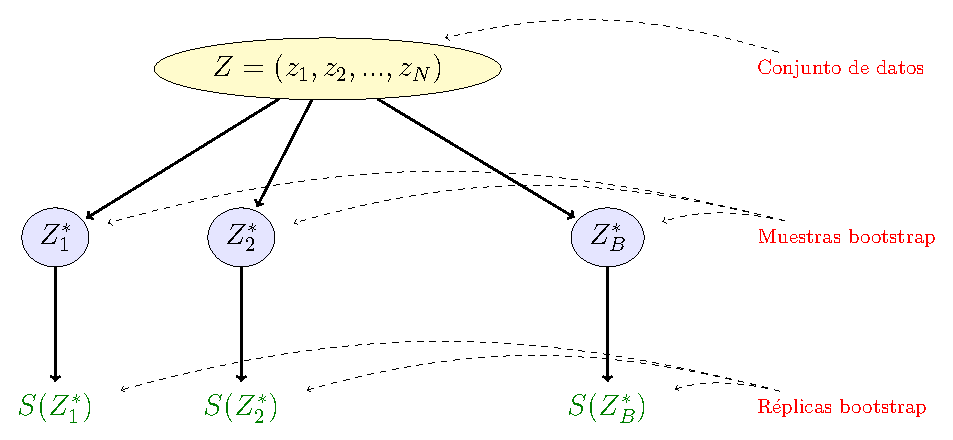
\includegraphics[width=1.1\linewidth]{gfx/chap4/untitled}}        
  \caption[Esquema del proceso bootstrap.]{Esquema del proceso bootstrap. Se desea estimar la precisión del estadístico $S(\mb{Z})$. Para esto, se generan $B$ conjutos, cada uno muestreando con reemplazo $N$ elementos del conjunto original. A cada uno de estos $b = 1, 2, ..., B$ elementos se le denomina $\mb{Z}^{*}_b$, y es a partir de estos que se calcula el estadístico de interés. Usando estas réplicas bootstrap es como se estima la varianza del $S(\mb{Z})$ previamente calculado.}
  \label{fig:bootesq}
\end{figure}

Hay que observar que lo que hace bootstrap es realmente estimar la varianza muestral a partir de la distribución empírica $\hat F$ y conforme $B \rightarrow \infty$, $\widehat{Var}(\hat F)$ tiende a la varianza poblacional $\widehat{Var}(\hat F) = {Var}(\hat F)$ de la misma $\hat F$. Para que realmente $\widehat{Var}(\hat F)$ converja a  ${Var}(F)$ se necesita además que $N \rightarrow \infty$, es decir, que se tengan muestras infinitas de la distribución original.

El ejemplo anterior, así como la mayor cantidad de literatura disponible tratan sobre bootstrap como una técnica para estimar errores estándar o construir intervalos de confianza de un estadístico \cite{MacKinnon2007}. Sin embargo, en este caso se usará bootstrap para realizar pruebas de hipótesis de una cola, fijando un nivel de significancia $\alpha$ que más adelante se especificará.

\subsection{Bootstrap paramétrico}

Como ya se mencionó, el bootstrap clásico es no paramétrico, y se vale únicamente del conjunto observado para a partir de ahí estimar la función de distribución empírica. En el caso que nos interesa, se cuenta con un modelo paramétrico que ha sido ajustado a los datos, usualmente por \ac{MLE}. 

Entonces, a partir de este modelo ajustado es que se muestrea. Al igual que en con la técnica no paramétrica, se suelen generan muestras de datos del mismo tamaño que el conjunto original. Luego, para cada nueva conjunto bootstrap $\mb{Z}^{*}_b$ muestreado se calcula el estadístico de nuestro interés. Éste proceso de muestreo se repite igualmente una gran cantidad de veces. 

El método de bootstrap paramétrico se suele utilizar en problemas en los que se desea ajustar un modelo y además encontrar sus parámetros correspondientes. Nos permite ajustar de mejor forma los parámetros de un modelo, calculando algún estadístido de interés que permita analizar el comportamiento de cada uno de los parámetros estimados.

\section{Selección de modelo usando BIC}

Como ya se mencionó al principio de este capítulo, hay muchas formas de aboradar el problema de selección de modelo. En este trabajo se usará una combinación de los dos tipos presentados.

Puesto que consideramos que dentro de nuestro espacio de modelos propuestos se encuentra el modelo solución (esto es, hay un modelo que corresponde con el número de interlocutores que participan en la grabación), resulta más natural usar \ac{BIC}.

Esta función de penalización se calcula de la siguiente manera: 
\begin{equation}
BIC(\mc{M}) = 2 \mc{L}_{max}(\mc{M}) - (log N ) dim(M)
\end{equation}
para cada propuesta de modelo $\mc{M}$, donde $dim(M)$ es el número estimado de parámetros libres que le corresponden, y $N$ es el tamaño de nuestra muestra de datos. Por otra parte, $\mc{L}_{max}(\mc{M})$ es la máxima log-verosimilitud obtenida para el modelo $\mc{M}$ después de realizar un número $K$ se simulaciones, para evitar que en algún caso el algoritmo de estimación se quede atorado en un máximo local.

Para estimar el número de parámetros libres de nuestro modelo, se consideran todas las probabilidades que rigen al \ac{HMM}, que en este caso son: la matriz a priori o inicial, la matriz de transiciones entre los interlocutores, así como la matriz de emisión de cada persona para todo el diccionario de palabras.

Este tipo de función de penalización nos permite seleccionar de entre un conjunto de modelos propuestos (que pueden ser muchos) al modelo o los modelos con mayor probabilidad de ser los correctos. 

Se enfoca en escoger el modelo candidato con la mayor probabilidad dados los datos, pero penalizando la complejidad de cada propuesta. Se preferirán entonces los modelos con una mayor verosimilitud que involucren la menor cantidad de parámetros posibles. 

En caso de que dos o más modelos tengan una puntaje similar en \ac{BIC}, se buscará hacer un análisis más extenuante para revisar cuál modelo es más conveniente.

\section{Selección de modelo usando bootstrap con likelihood ratio testing}

Para esta otro propuesta, se utilizará la técnica bootstrap paramétrico, pues mediante el algoritmo \ac{EM} es fácil obtener el modelo parametrizado. El estadístico a evaluar será el \ac{LLR}, que nos permitirá comparar entre dos modelos propuestos. 

Usualmente se compararán dos modelos adyacentes, es decir, el modelo $\mc{M}_d$ de $d$ estados contra el modelo $\mc{M}_{d+1}$ de $d+1$ estados ocultos.

La prueba que se realiza es comparando el \ac{MLE} $\hat \theta^{(d)}$ y $\hat \theta^{(d+1)}$ de los modelos de $d$ y $d+1$ estados respectivamente. Para la comparación se usa la estadística \ac{LLR} que corresponde a la diferencia de las log-verosimilitudes mencionadas
\begin{equation}
  LLR^{(d)}_{obs} = log \frac{L(\hat \theta^{(d+1)}; y_{1:n})}{L(\hat \theta^{(d)}; y_{1:n})} =
    log L(\hat \theta^{(d+1)}; y_{1:n}) - 
    log L(\hat \theta^{(d)}; y_{1:n})
\end{equation}

Para calcular el \ac{MLE} de un modelo, se estimó la verosimilitud varias veces con diferentes parámetros iniciales aleatorios. Se iteró el algoritmo \ac{EM} hasta convergencia, un numero $iter_{hmm}$ fijo de iteraciones, esto para evitar el estancamiento del algoritmo en un máximo local, y obtener así una buena estimación de la máxima verosimilitud del modelo.

Se usó entonces como \ac{MLE} del modelo la máxima verosimilitud correspondiente a los mejores parámetros estimados y que se denotó por $LLR_{obs}$.

Ahora, para hacer la prueba con bootstrap se simularán datos de los \ac{HMM} propuestos, utilizando el algoritmo \ref{alg:ancsamp} para el muestreo, tanto para el modelo $\mc{M}_d$ como para el modelo $\mc{M}_{d+1}$. Para ambos modelos se estimará su log-verosimilitud y se procederá con el cálculo del \ac{LLR}, que es la réplica bootstrap que nos interesa. 

\begin{algorithm}[tp]
   \caption{Muestreo ancestral para un HMM}
   \label{alg:ancsamp}
\begin{algorithmic}
   \STATE {\bfseries Input:} \\
   núm. de estados $N$, núm. de muestras en el tiempo $T$ \\
   núm. de posibles valores en el diccionario $K$, \\
   $ \pi \in \mathcal{R}^{N}; ~~ \pi_j = p(z_{1j})$ \\
   $ \mathbf{A} \in \mathcal{R}^{N \times N}; ~~
   \mathbf{A}_{jk} = p(z_{nk} \,|\, z_{n-1, j})$ \\

   $ \mathbf{B} \in \mathcal{R}^{K \times N}; ~~
   \mathbf{B}_{jk} = p(x_{nk} \,|\, z_{n, j})$\\  
   \STATE
   \STATE $z_1 \sim Multinomial(\pi)$   
   \STATE $x_1 \sim Multinomial(\mathbf{E}_{[z_1,~:]})$

   \FOR{$i = 1 \to T$} 
    \STATE $z_t \sim Multinomial(\mathbf{A}_{[z_{t-1},~:]})$ 
    \STATE $x_t \sim Multinomial(\mathbf{B}_{[z_t,~:]})$
   \ENDFOR   
\end{algorithmic}
\end{algorithm}

Para cada par de modelos $\mc{M}_d, \mc{M}_{d+1}$ se realizará este procedimiento $B$ veces: muestreando ambos modelos, estimando su verosimilitud y calculando el estadístico $\ac{LLR}$. Para cada simulación bootstrap se generará un $LLR_{boot}^b$ referente a la muestra generada. 

Cuando se termine el proceso bootstrap, se tendrán $\lbrace LLR_{boot}^b \rbrace_{b=1}^B$ estadisticos, y se podrá generar una densidad sobre los valores de $LLR_{boot}^b$. 

La última etapa será realizar una prueba de hipótesis para ver si el valor $LLR_{obs}$ tiene la misma distribución que los $\lbrace LLR_{boot}^b \rbrace_{b=1}^B$. La hipótesis nula será que el modelo $\mc{M}_d$ es el modelo correcto, y entonces el valor $LLR_{obs}$ estará en el rango mismo de los $LLR_{boot}$. Sin embargo, si se rechaza la hipótesis nula (de acuerdo a un nivel de significancia establecido) significará que el modelo $\mc{M}_{d+1}$ es mejor que el $\mc{M}_{d}$.

\cleardoublepage
\part{Marco experimental}
\clearpage

%!TEX root = ../Thesis.tex

\chapter{Metodología}\label{ch:chap5}

\epigraphhead[70]{
\epigraph{There was nowhere to go but everywhere, so just keep on rolling under the stars.}
{Jack Kerouac}}

A continuación se describe la metodología que se llevó a cabo para la tarea de \sd. 

Como ya se describió en el \autoref{ch:chap2} es necesaria una etapa de pre-procesamiento en el sistema; primero para eliminar de la señal de audio las cosas que no nos interesan (que en este caso son silencios), para lo que se usó un detector de energía y así ignorar los instantes en los que ningún interlocutor participa. 

Luego, también en la etapa de pre-procesamiento se encuentra el obtener vectores de características que representen de alguna manera la señal, y que sean mucho más fáciles de manipular. Para esta etapa se usaron los \ac{MFCC}, siguiendo el algoritmo \autoref{alg:mfcc}.  Después de obtener los vectores característicos, se agruparon mediante k-means++ (\autoref{alg:kmeanspp}) para de alguna forma discretizar todas las posibles palabras emitidas en el diálogo. Esta agrupación inicial nos permitirá reducir la dimensionalidad de los vectores, así como aglomerar aquellos que sean muy similares con respecto a los demás.

Después de esta etapa de clasificación, ya se tendrán los datos como observaciones que representarán las variables observadas del \ac{HMM}. Como se desconoce tal cual el número de personas involucradas en la grabación, se propondrán varios modelos $\mc{M}_d$ con $d$ estados ocultos. El valor de $d$ variará de acuerdo a qué tan extensas se deseen hacer las pruebas, pero a priori no hay un límite pre-establecido. 

Luego, corresponderá usar el algoritmo \ac{EM} con cada uno de los modelos $\mc{M}_d$ propuestos, tanto para estimar sus parámetros como para estimar su verosimilitud. Como ya se mencionó en \autoref{ch:chap4} esta etapa se realizará varias veces, para evitar el estancamiento del método y obtener un buen ajuste del modelo. Del modelo con mayor versomilitud se calculará la segmentación correspondiente, y se almacenará. 

Después, seguirá la etapa de selección de modelo. Este proceso se realizará en dos partes: primero, explorando todo el espacio de soluciones y reduciendo los posibles modelos ganadores; y luego, seleccionando de entre los candidatos resultantes al mejor modelo.

En un primero paso, se estimará \ac{BIC} para todos los \ac{HMM} propuestos para generar una curva de selección. Como se verá en las pruebas, es necesario introducir un término de regularización en \ac{BIC} para que la penalización del modelo corresponda con las log-verosimilitudes obtenidas. 

Esto se puede hacer de la siguiente forma: 
\begin{equation}
BIC_{\lambda}(\mc{M}) = 2 \mc{L}_{max}(\mc{M}) - \lambda \cdot log N \cdot dim(M)
\end{equation}
aunque presenta el inconveniente de tener que encontrar el valor adecuado para $\lambda$ que penalice de buena forma los modelos. 

Para escoger el valor adecuado de $\lambda$ se realizará un análisis de sensibilidad, generando múltiples curvas de selección \ac{BIC} con diferentes valores de $\lambda$. Tanto la discretización como los rangos de $\lambda$ permitirán hacer una mejor búsqueda del parámetro. Con todas estas diferentes curvas, se tendrá una superficie, en donde en un eje variará el número de interlocutores del modelo, mientras que en el otro será el valor de regularización $\lambda$ el que cambiará. 

Se busca mediante este análisis encontrar la región de inflexión que divide a la superficie en dos: en la primera parte de la superficie, el valor de $\lambda$ será pequeño, por lo que siempre tendrán una mayor verosimilitud los modelos con más parámetros; mientras que en la segunda parte, la penalización sera muy grande, y se escogerán siempre los modelos más sencillos, sin darle tomar en cuenta su verosimilitud.

Por esto mismo, se puede calcular el gradiente de la superficie generada por las funciones \ac{BIC}, y se buscará la región el valor de $\lambda$ en el que la suma de los valores absolutos sea menor. 

Es importante recordar que el modelo \ac{HMM} al ser resuelto usando \ac{EM} buscará siempre maximizar la función de verosimilitud; por lo que es natural que mientras más parámetros tenga un modelo, mejor será su ajuste a los datos y mayor su verosimilitud.

Basándonos en esto, si se comparan distintos modelos con un $\lambda$ pequeño, se espera que los modelos más complejos sean los que tengan un valor \ac{BIC} mayor; por lo que habrá un gradiente en esa dirección con pendiente positiva. Por otro lado, cuando el $\lambda$ sea demasiado grande, los modelos más sencillos seran los que tengan asociado un valor de \ac{BIC} mayor; y entonces el gradiente estará en el otro sentido, con una pendiente negativa. 

El caso que nos interesa es cuando el valor de $\lambda$ penaliza de forma correcta, es decir, está en el mismo orden de magnitud que la mayoría de las verosimilitudes de los modelos. En ese momento, el gradiente de la superficie deberá tener dos direcciones, pues el valor máximo de \ac{BIC} no corresponderá al modelo más simple o al más complicado. Y además, la suma de los gradientes para ese valor será menor con respecto a otros valores de $\lambda$. 

Una vez que se logre seleccionar el $\lambda$ adecuado de regularización, se procede a evaluar su curva \ac{BIC} asociada y de ahí se obtiene al modelo ganador o un subconjunto de posibles ganadores (en caso de que varios modelos tengan puntuaciones similares de acuerdo a \ac{BIC}).

Como ya se mencionó, en el segundo paso, se realizará un proceso de refinamiento en caso de que se tengan varios modelos posibles. Para esto, se formarán pares de modelos que se deseen comparar, y se estimará su \ac{LLR}, que se denominará como $LLR_{obs}$. Para este mismo par de modelos, y mediante bootstrap paramétrico se hará una prueba de hipótesis para comproar cuál modelo es más adecuado para los datos.

Esto es, a partir de los dos modelos a examinar, se simularán múltiples secuencias de datos con los parámetros que se estimaron para cada modelo; y luego, con los datos simulados se estimará su máxima verosimilitud, para luego calcular el \ac{LLR}, que ahora se denominará $LLR_{boot}$. 

Como esta simulación se harán muchas réplicas, y con todos los valores $LLR_{boot}$ que se obtengan se formará una curva. Mediante una prueba de hipótesis se revisará si el $LLR_{obs}$ tiene la misma distribución que la curva de $LLR_{boot}$. La hipótesis nula corresponderá a que el primer modelo sea el correcto, y entonces tanto $LLR_{boot}$ como $LLR_{obs}$ tengan la misma distribución. Por otro lado, la hipótesis alternativa significaría que se rechaza $LLR_{obs}$ como una muestra de $LLR_{boot}$ bajo una significancia dada; y entonces se rechaza que el primer modelo sea el correcto.

De esta forma, se pueden realizar pruebas de hipótesis para los modelos candidatos, e ir rechazando modelos de acuerdo al análisis propuesto. En el \autoref{ch:chap6} se describe más a detalle esta selección de moledo, con las pruebas realizadas.

\section{Esquema general} 

El esquema general con las diferentes etapas que se realizan para estimar el número de personas así como su segmentación correspondiente.

\begin{figure}[bth]
  \centerline
  {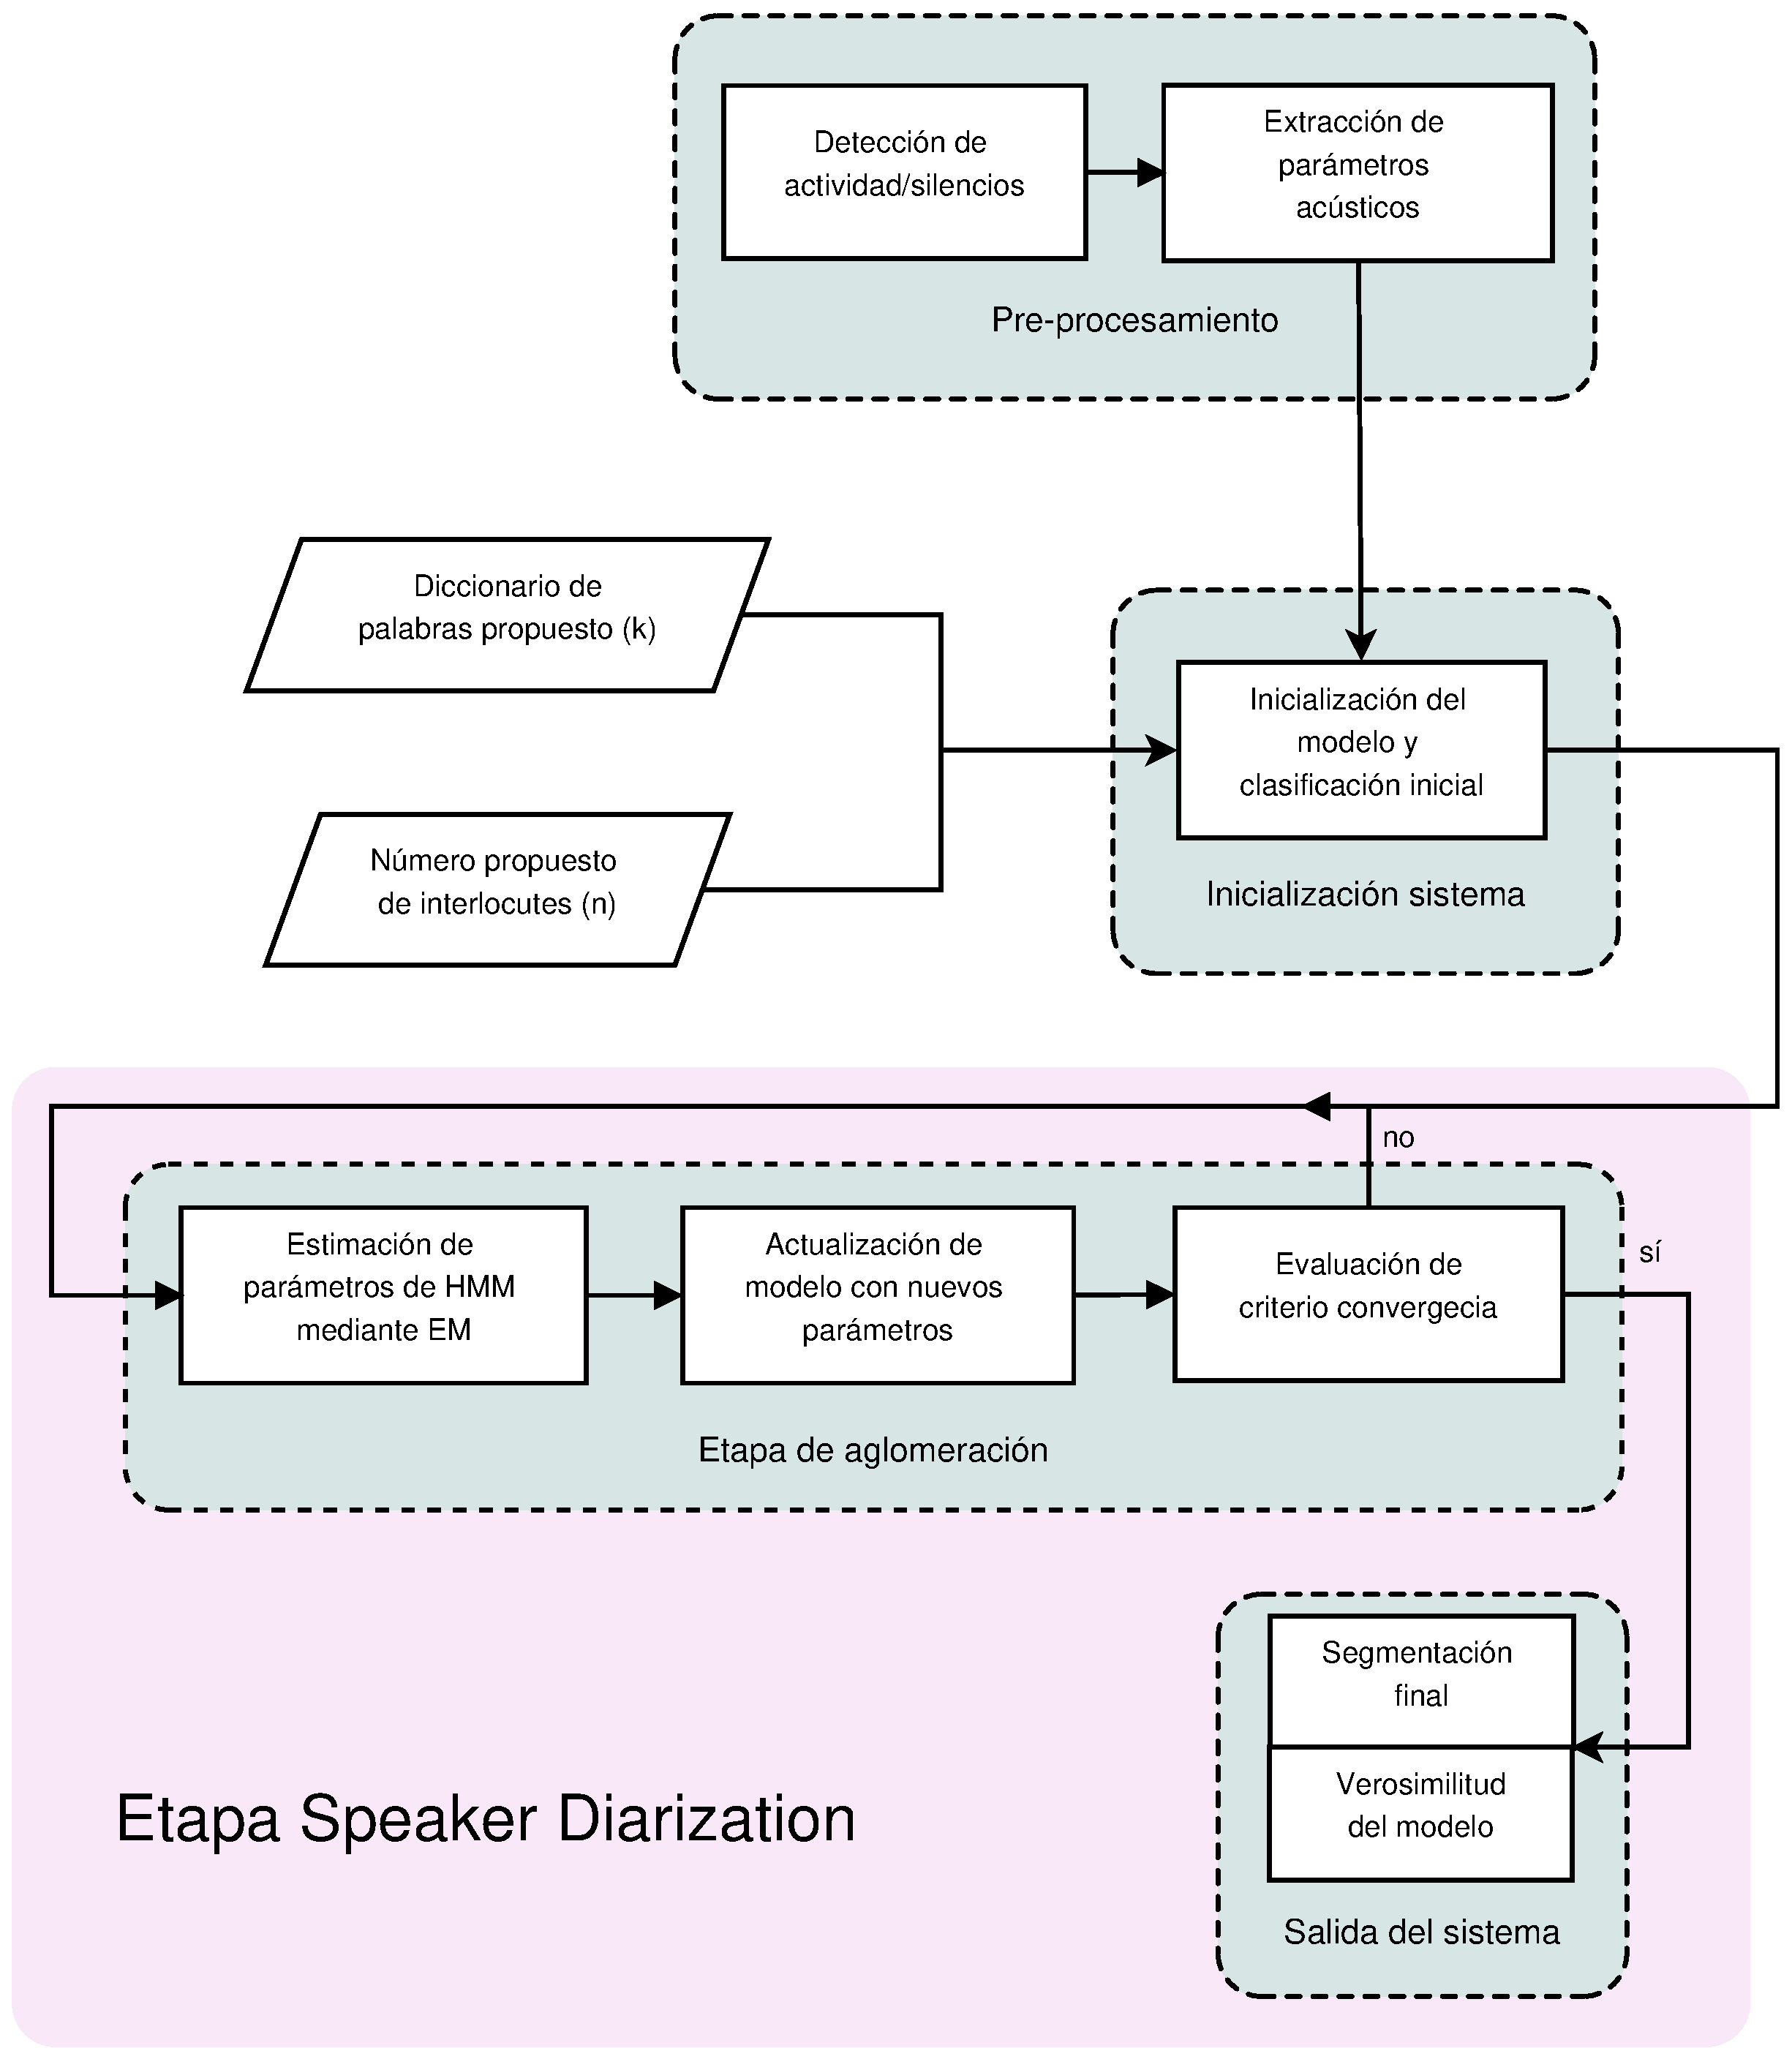
\includegraphics[width=1.5\linewidth]{gfx/chap5/general_flow}} \quad
  \caption{Esquema general.}
  \label{fig:esquema2}
\end{figure}

%!TEX root = ../Base.tex

\chapter{Experimentos y resultados}\label{ch:chap5}

En los capítulos anteriores se ha descrito los diferentes algoritmos que se utilizarán para realizar la tarea de \sd, y que en esta sección se emplearán de acuerdo al marco experimental que se describe a continuación.

Inicialmente, las pruebas consistieron en usar los algoritmos presentados para selección de modelo usando datos que fueron generados aleatoriamente a partir de los parámetros de un HMM inicial; para tener una idea general de su desempeño individual.

Para estas primeras pruebas, se simuló una cadena de Márkov oculta con base en parámetros fijos, generando tanto una secuencia de datos observados, como los supuestos datos o variables ocultas que forman la cadena de Márkov. Se utilizó muestreo ancestral para la simulación de estos datos.

Para un caso en específico, se tiene lo siguiente. Realizando la inferencia de parámetros del HMM, se obtienen los siguientes resultados:

El primer algoritmo que se prueba, es el de selección de modelo usando un BIC.

Como ya se comentó, se usará una variante de BIC en donde se incorpora un término de regularización $\lambda$ para que correspondan en órdenes de magnitud tanto la log-verosimilitud del modelo encontrado como su penalización respectiva.

El problema inmediato que se presenta, es cómo realizar la selección del parámetro de regularización $\lambda$ que penalice de forma correcta la verosimilitud para los diferentes modelos propuestos. Si $\lambda$ es demasiado pequeño, entonces la penalización realmente no tendrá efecto y dado el sobre ajuste que se presenta al usar modelos más complejos, se preferirán siempre los modelos con más parámetros. Por otro lado, si al escoger $\lambda$ se da demasiado peso al término de penalización, entonces siempre se preferirán los modelos más sencillos.

Para encontrar el valor de $\lambda$ adecuado, se puede entonces formar una superficie con las diferentes curvas de selección BIC de acuerdo a cómo varía $\lambda$, e inspeccionar esta superficie para encontrar una región de confianza en la que el valor de $\lambda$ es el adecuado.

Por otro lado, para la segunda prueba, se procedió a usar bootstrap con la estadística log-likelihood ratio como ya se describió anteriormente en el \autoref{ch:chap3}, y haciendo la prueba de hipótesis del modelo de $n$ estados contra el de $n+1$ estados.

\section{Experimentos} % (fold)
\label{sec:experimentos}

Para los experimentos realizados, se generaron mediante un sintetizador de voz (también conocido como Text-To-Speech o TTS por sus siglas en inglés) para la generación de las Secuencias de prueba, lo que nos permitió tener un mayor control sobre el contenido como tal de las grabaciones, así como sobre los posibles ruidos o interferencias en la señal de audio.

Si bien, para probar el desempeño contra otras propuestas del estado del arte se suelen usar otro tipo de bases de datos (tales como NIST, ...), éstas suelen no estar disponibles de forma libre, por lo que preferimos generar nosotros un conjunto de pruebas con el sintetizador de voz.

Usando dos motores para el sintetizador de voz, uno con voces en inglés y otro con voces en español, se generaron 6 secuencias de audio (3 en cada idioma) cuya duración así como el número de interlocutores que participan varía.

\subsection[Secuencia 1]{Secuencia 1: Edgar Allan Poe} % (fold)
\label{ssub:allanpoe}

  En esta primer secuencia se tomaron varios poemas del escritor Edgar Allan Poe, y se utilizaron 6 diferentes voces en inglés. La secuencia de audio original es de 12:06 min.

Para la etapa de agrupación de los vectores MFCC con k-means++ se usaron 140 centros iniciales, mientras que el banco de filtros fue el mismo que anteriormente se mencionó.

\begin{figure}[tp]
  \centerline{  
    \hspace{1.2cm}
    \parbox[c]{0.38\textwidth}{\centering Modelo generador}
    \parbox[c]{0.38\textwidth}{\centering Modelo $n_4$}
    \parbox[c]{0.38\textwidth}{\centering Modelo $n_5$}
    \parbox[c]{0.38\textwidth}{\centering Modelo $n_6$}
  }
  \vspace{0.5cm}
  \foreach \row in {1, ..., 2}{%  
    \centerline{%
      \parbox[c]{1cm}{
        \vspace{-0.5cm}
        \myheader{\row}
      }
      %\gdef \widthimg {0.35}
      \foreach \col in {1, ..., 4}{%
        \pgfmathparse{\col == 4 && \row == 2? 1:0}
        \ifthenelse{\pgfmathresult=1}{
          \gdef \widthimg {0.39}
        }{
          \gdef \widthimg {0.35}
        }
        \begin{subfigure}[c]{\widthimg \textwidth}          
          \def \imgfile {gfx/chap6/cuervo1p_\col_\row}
          \IfFileExists{\imgfile.eps}{
            \includegraphics[width=1\textwidth]{\imgfile}
            \label{fig:seq1p_\col_\row}
          }{
            \hspace{1\textwidth}
          }
        \end{subfigure}
        %\hspace{-0.005\textwidth}
      }
    }
  }
\caption[Secuencia 1: Parámetros estimados (1)]{Por columnas, se muestran los parámetros obtenidos para varios modelos propuestos. La primer columna corresponde a los parámetros verdaderos.
En la primer fila \textup{(a)} se muestran las probabilidades a priori de que cada uno de los interlocutores empiecen la conversación. En la segunda fila \textup{(b)} se muestra en falso color la matriz de transición entre interlocutores para cada uno de los modelos mostrados.}
\label{fig:seq1p}
\end{figure}

En las \autoref{fig:seq1p} y \autoref{fig:seq1q} se muestran los parámetros estimados para los diferentes modelos que se propusieron. La primer columna corresponde a los parámetros verdaderos, mientras que las demás columnas son los parámetros obtenidos para diferentes modelos estimados. 

En la primer fila de la \autoref{fig:seq1p} se muestran las probabilidades a priori de que cada uno de los interlocutores empiecen el diálogo. En la segunda fila se muestra en falso color la matriz de transición para cada uno de los modelos. Esta matriz representa la probabilidad de cambio entre las personas que participan en la conversación.

Se observa como en general para todos los modelos propuestos la matriz de transición que se recupera tiene una estructura diagonal, puesto que en este tipo de problemas, una persona suele hablar durante un periodo considerablemente largo, para que luego otra persona empiece a hablar.

\begin{figure}[t!]
  \centerline{
    \hspace{1.2cm}
    \parbox[c]{0.35\textwidth}{\centering Modelo generador}
    \parbox[c]{0.35\textwidth}{\centering Modelo $n_4$}
    \parbox[c]{0.35\textwidth}{\centering Modelo $n_5$}
    \parbox[c]{0.35\textwidth}{\centering Modelo $n_6$}
  }
  \vspace{0.5cm}
  \foreach \row in {3, ..., 9}{%  
    \centerline{
      \parbox[c]{1cm}{
        \vspace{-0.3cm}
        \myheader{\row}
      }
      \foreach \col in {1, ..., 4}{%
        \begin{subfigure}[c]{0.35\textwidth}  
          \def \imgfile {gfx/chap6/cuervo1p_\col_\row}
          \IfFileExists{\imgfile.eps}{
            \includegraphics[width=1\textwidth]{\imgfile}
            %\caption{}
            \label{fig:seq1p_\col_\row}
          }{
            \hspace{1\textwidth}
          }
        \end{subfigure}
      }
    }
  }
\caption[Secuencia 1: Parámetros estimados (2)]{Por columnas, se muestran las probabilidades de emisión para cada uno de los interlocutores de acuerdo al modelo. Cada fila representa las probabilidad de emisión de las palabras en el diccionario. La fila \textup{(c)} para la primer persona, la fila \textup{(d)} para la segunda persona y así de forma consecutiva, de acuerdo al número de personas que contempla cada modelo propuesto.}
\label{fig:seq1q}
\end{figure}

En la \autoref{fig:seq1q} se muestran las probabilidades de emisión para cada uno de los participantes, de acuerdo a las palabras en las que se ha discretizado la conversación, como se explicó anteriormente en el algoritmo a\autoref{alg:kmeanspp}. Idealmente, cada interlocutor tiene asignadas con mayor probabilidad un cierto conjunto de palabras del diccionario, lo que hace que la identificación de las personas sea mucho más fácil de realizar.

Para la selección del modelo y siguiendo la metodología propuesta, primero se efectúa una inspección por medio de \ac{BIC} regularizado para encontrar cuál o cuáles son los modelos más probables.

\begin{figure}[t!]
  \centerline{
  \begin{subfigure}[b]{1.1\textwidth}
   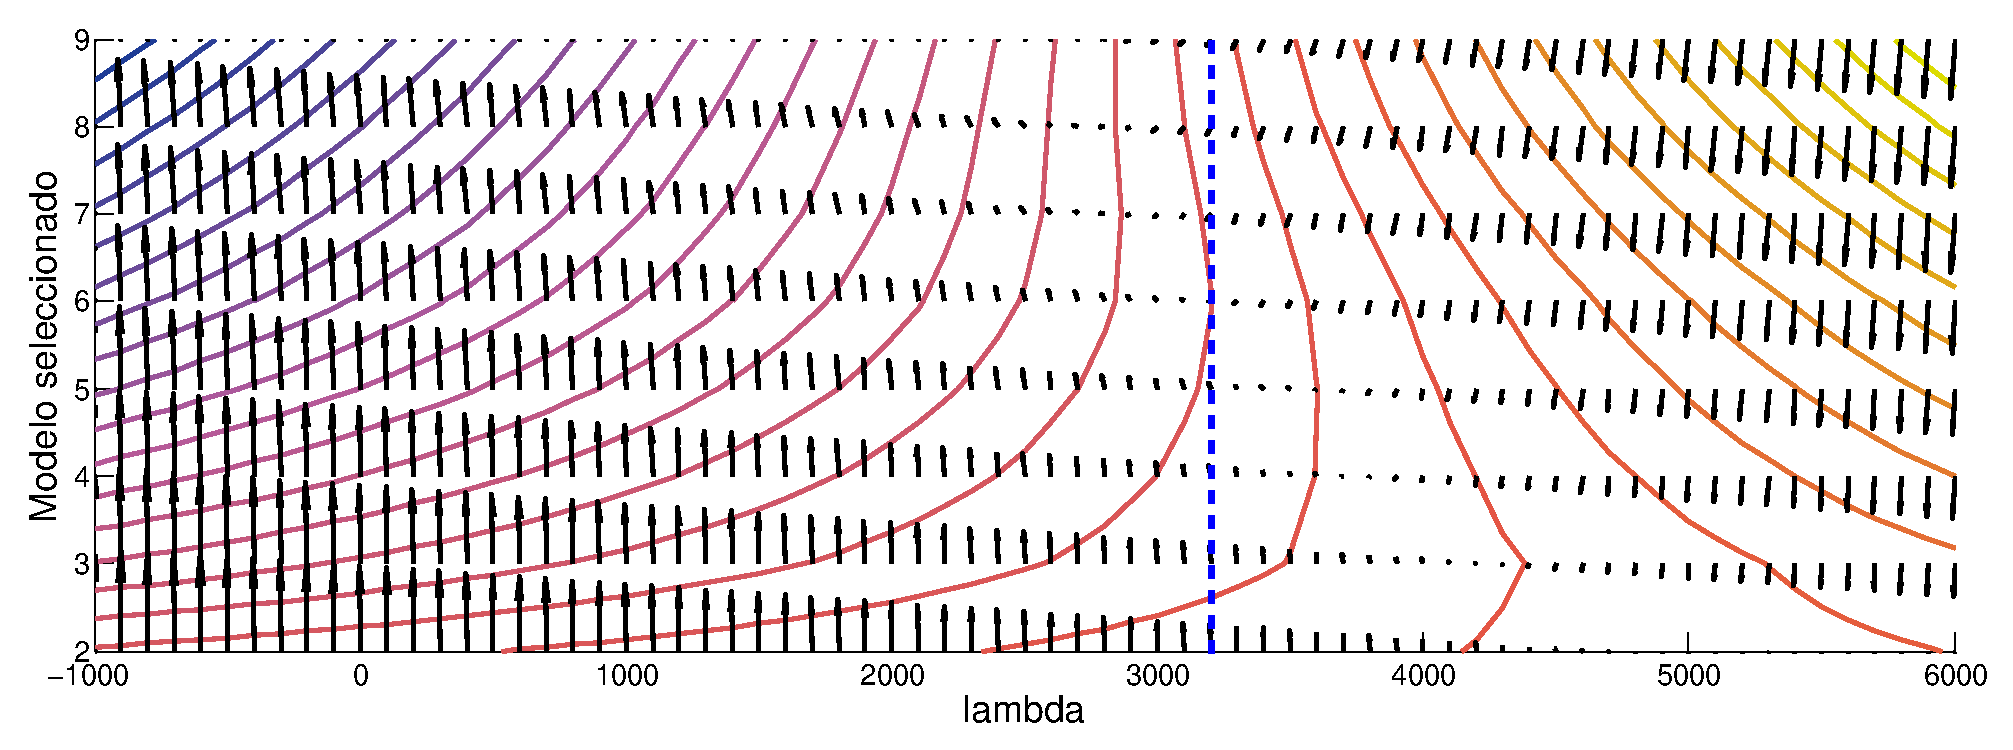
\includegraphics[width=1\textwidth]{gfx/chap6/cuervo1bic2}
   \caption{}
   \label{fig:seq1_bic2}
  \end{subfigure}  
  }  
  \centerline{
  \begin{subfigure}[b]{0.55\textwidth}
    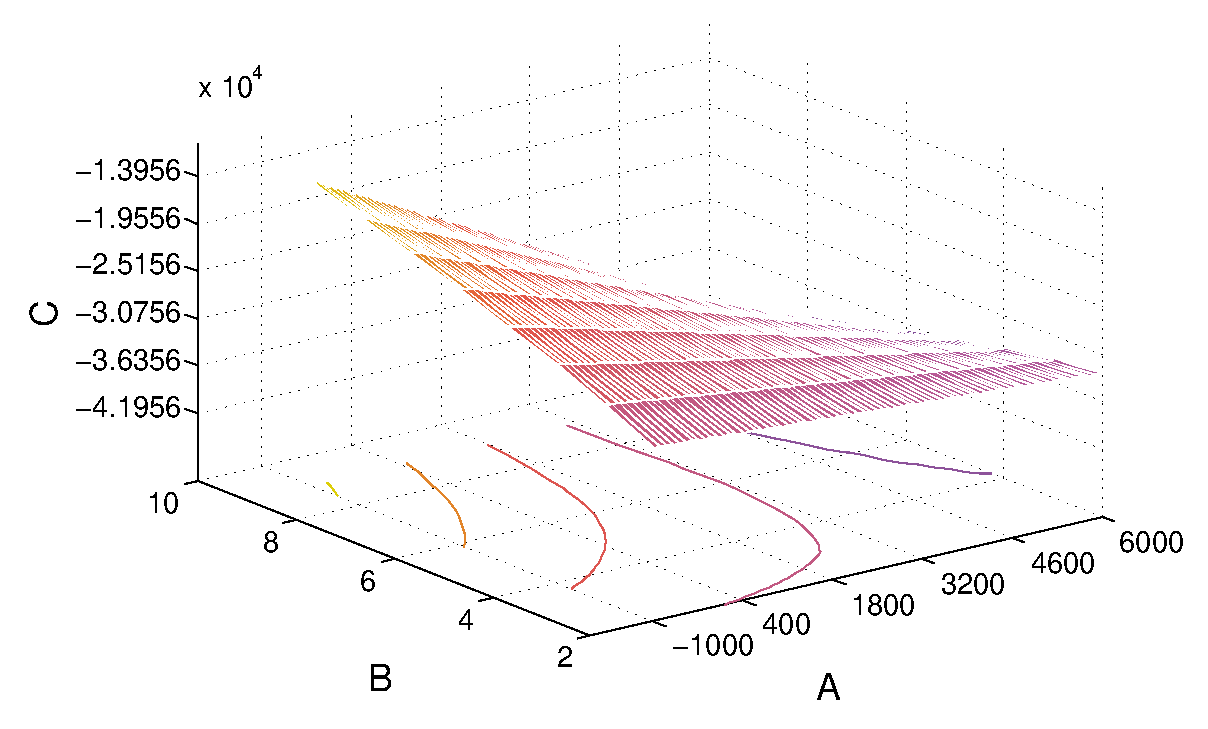
\includegraphics[width=\textwidth]{gfx/chap6/cuervo1bic1} 
    \caption{}
    \label{fig:seq1_bic1}
  \end{subfigure}  
  \begin{subfigure}[b]{0.55\textwidth}
    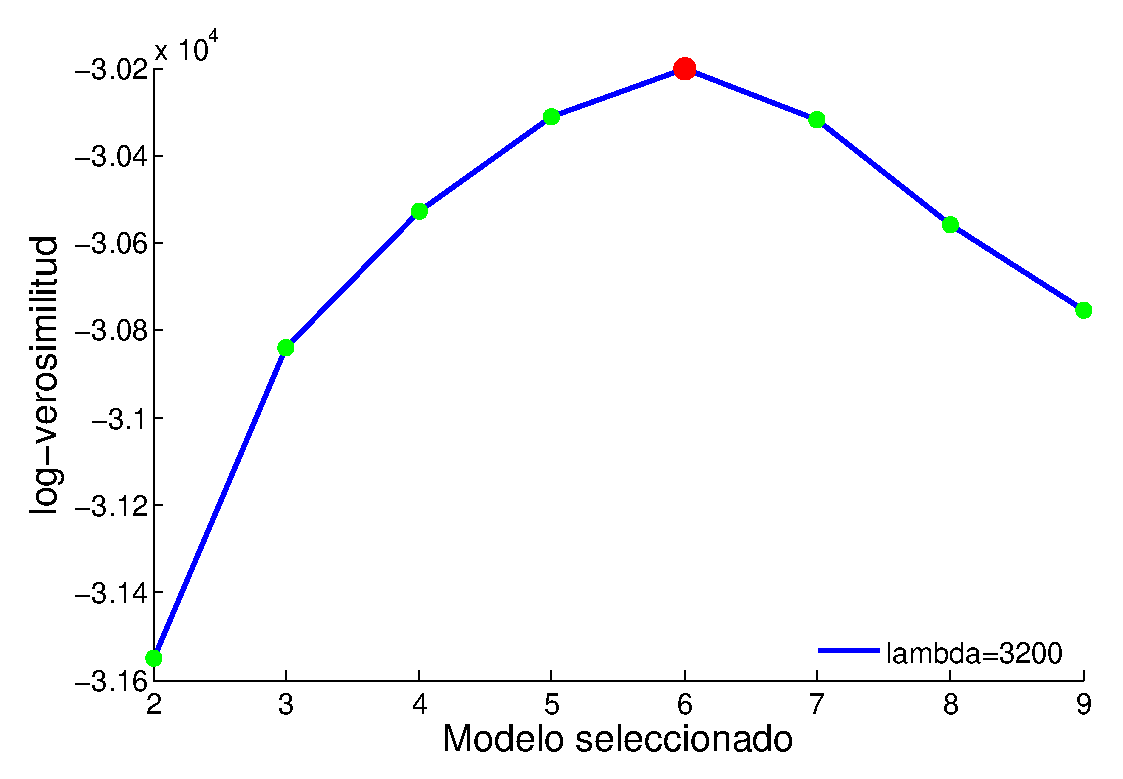
\includegraphics[width=\textwidth]{gfx/chap6/cuervo1bic3} 
    \caption{}
    \label{fig:seq1_bic3}
  \end{subfigure}
  }
  \caption[Secuencia 1: Pruebas BIC]{En la \autoref{fig:seq1_bic2}, se muestra las curvas de nivel de la superficie al variar el valor de lambda para evaluar BIC, así como la dirección del gradiente en la misma. En la \autoref{fig:seq1_bic1} se muestra una perspectiva general de superficie en \autoref{fig:seq1_bic2}. En la \autoref{fig:seq1_bic3} se muestra el valor seleccionado para lambda de acuerdo al análisis de sensibilidad realizado en la superficie anterior.}
  \label{fig:seq1_bic}
\end{figure}

En la \autoref{fig:seq1_bic1} se muestra la superficie generada al variar el valor de $\lambda$ para diferentes curvas de selección BIC. Se observa cómo al principio $\lambda$ es muy pequeño, y entonces el término de penalización no funciona por lo que se prefieren los modelos más complejos y sobre ajustados. Por otro lado, cuando $\lambda$ es muy grande, la penalización no permite mas que escoger los modelos más simples.

Haciendo un análisis de sensibilidad se puede determinar cuál es el parámetro $\lambda$ adecuado que penaliza de buena forma la log-verosimilitud.

En la \autoref{fig:seq1_bic2} se muestran las curvas de nivel de la figura anterior, además de la dirección del gradiente de la misma. Así mismo, en falso color se resaltan las zonas en las que el gradiente es menor. 

Lo que nos interesa encontrar en la superficie, es el valor de $\lambda$ que representa el punto de inflexión entre la selección de modelos demasiado complejos y modelos más simples. Para esto, se busca la zona en la que el gradiente sea lo más cercano a cero, pues implicaría que es un punto crítico.

Debido a la escala y a la forma en la que se calculó el gradiente, aunque para algunos valores cercanos de $\lambda$ no haya mucha variación en esa dirección; si \ac{BIC} está penalizando mal, entonces sí habrá gran variación para los diferentes modelos. Es por esto, que sólo en la zona en que la penalización sea del mismo orden de magnitud que la verosimilitud la variación en la curva \ac{BIC} con el $\lambda$ adecuado no será tan grande como en otras zonas.

Por último, se muestra en \autoref{fig:seq1_bic3} la curva BIC con el valor de $\lambda$ encontrado a partir del análisis de sensibilidad realizado en la \autoref{fig:seq1_bic2}. El o los modelos que tengan un mayor valor \ac{BIC} serán los que se seleccionarán como modelos ganadores.

\begin{figure}[t!]
  \centerline  
  { \begin{subfigure}[b]{0.7\textwidth}
      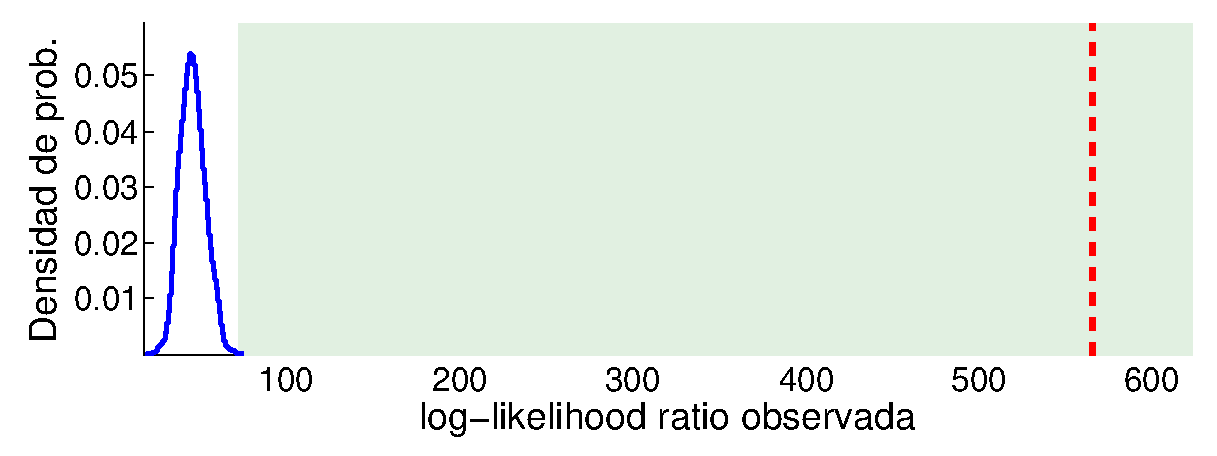
\includegraphics[width=1\linewidth]{gfx/chap6/cuervo1boot1}
      \caption{}
      \label{fig:seq1_boot1}
    \end{subfigure}
    \hspace{0.5cm}
    \begin{subfigure}[b]{0.7\textwidth}
      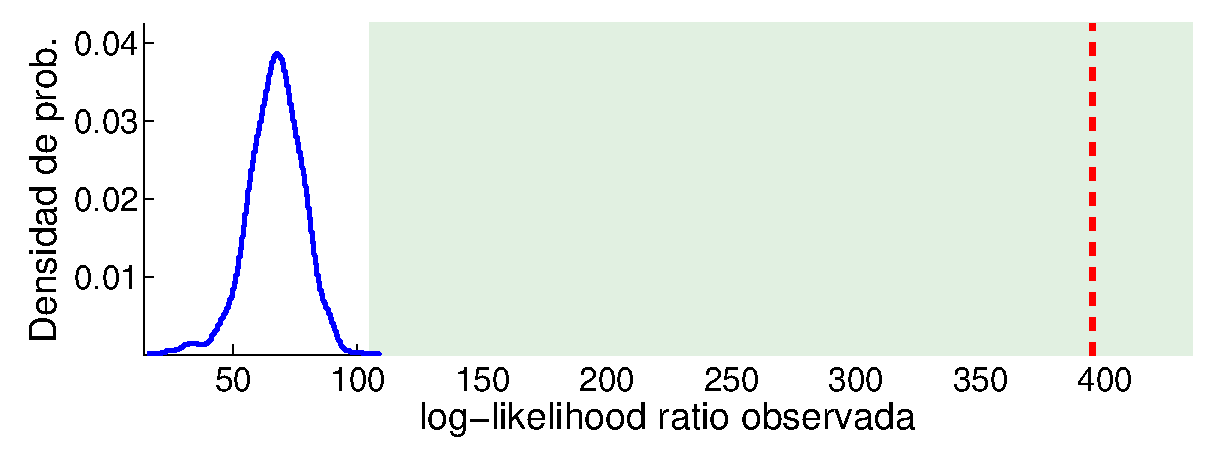
\includegraphics[width=1\linewidth]{gfx/chap6/cuervo1boot2}
      \caption{}
      \label{fig:seq1_boot2}
    \end{subfigure}
  }
  \centerline  
  { \begin{subfigure}[b]{0.7\textwidth}
      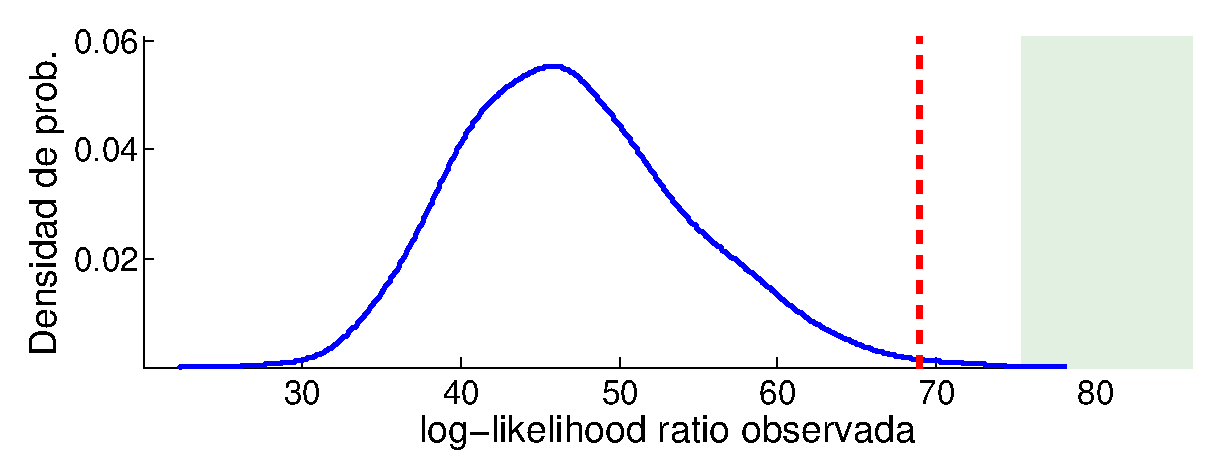
\includegraphics[width=1\linewidth]{gfx/chap6/cuervo1boot3}
      \caption{}
      \label{fig:seq1_boot3}
    \end{subfigure}
    \hspace{0.5cm}
    \begin{subfigure}[b]{0.7\textwidth}
      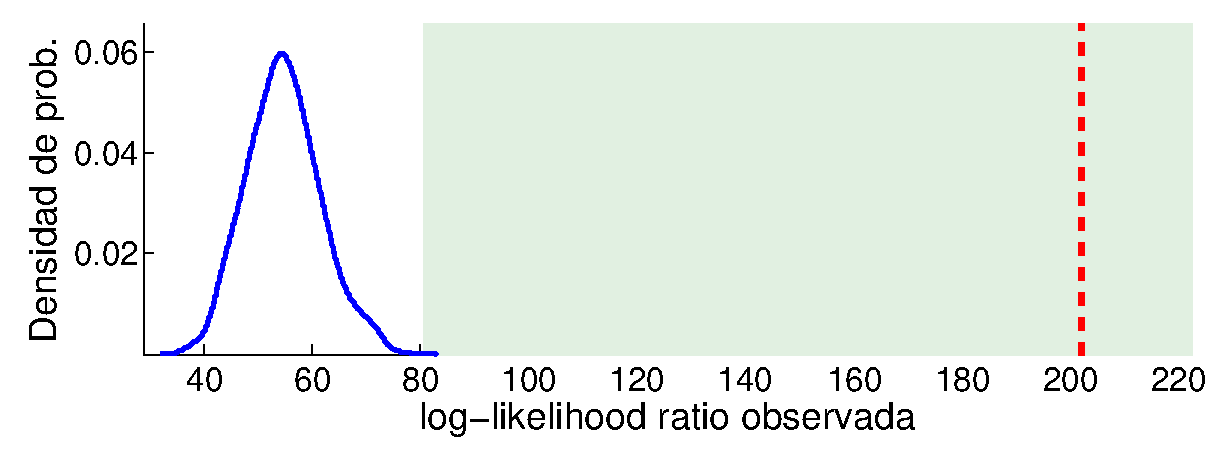
\includegraphics[width=1\linewidth]{gfx/chap6/cuervo1boot4}
      \caption{}
      \label{fig:seq1_boot4}
    \end{subfigure}
  }
  \caption[Secuencia 1: Pruebas de hipótesis usando bootstrap]{En la \autoref{fig:seq1_boot1} se muestra la prueba de hipótesis realizada para comparar el modelo $n_4$ contra $n_5$. Como se observa, se rechaza la hipótesis de que el modelo correcto sea $n_4$. En la \autoref{fig:seq1_boot2} se hace la prueba del modelo $n_5$ contra $n_6$, y de la misma manera, se rechaza la hipótesis de que el modelo correcto sea $n_5$. Se sigue con la prueba de hipótesis del modelo $n_6$ contra $n_7$ en la \autoref{fig:seq1_boot3}, y en este caso el valor observado no cae dentro de la región de rechazo, por lo que no podemos rechazar que el modelo $n_6$ sea el correcto. Por último en la \autoref{fig:seq1_boot4}, se hace la prueba del modelo $n_7$ contra el modelo $n_8$, y se vuelve a rechazar la hipótesis nula.}
  \label{fig:seq1_boot}
\end{figure}

En caso de que después de utilizar \ac{BIC} se presente ambigüedad para determinar un modelo ganador, o ya sea para realizar un análisis más exhaustivo, se puede propone hacer una prueba de hipótesis para determinar cuál modelo se ajusta mejor a los datos.

A diferencia de la primer etapa, en la que se usa \ac{BIC} como criterio para  seleccionar el mejor modelo de un conjunto no definido de modelos con diferentes parámetros, la intención de hacer pruebas de hipótesis es determinar en un pequeño conjunto de probables modelos, cuál es mejor, y qué tan bueno es un modelo respecto a otro.

Al plantear la prueba de hipótesis se harán una gran cantidad de simulaciones para ver qué tan bien se ajusta cada modelo a los datos originales, por lo que este proceso es computacionalmente intensivo y sólo se recomienda hacerlo para evitar la ambigüedad entre un par de modelos.

Por último, ya con el modelo seleccionado, se compara la segmentación recuperada con la secuencia o la segmentación originalde la conversación:
\begin{figure}[tp]
  \centerline
  {\begin{subfigure}[b]{1.3\textwidth}
      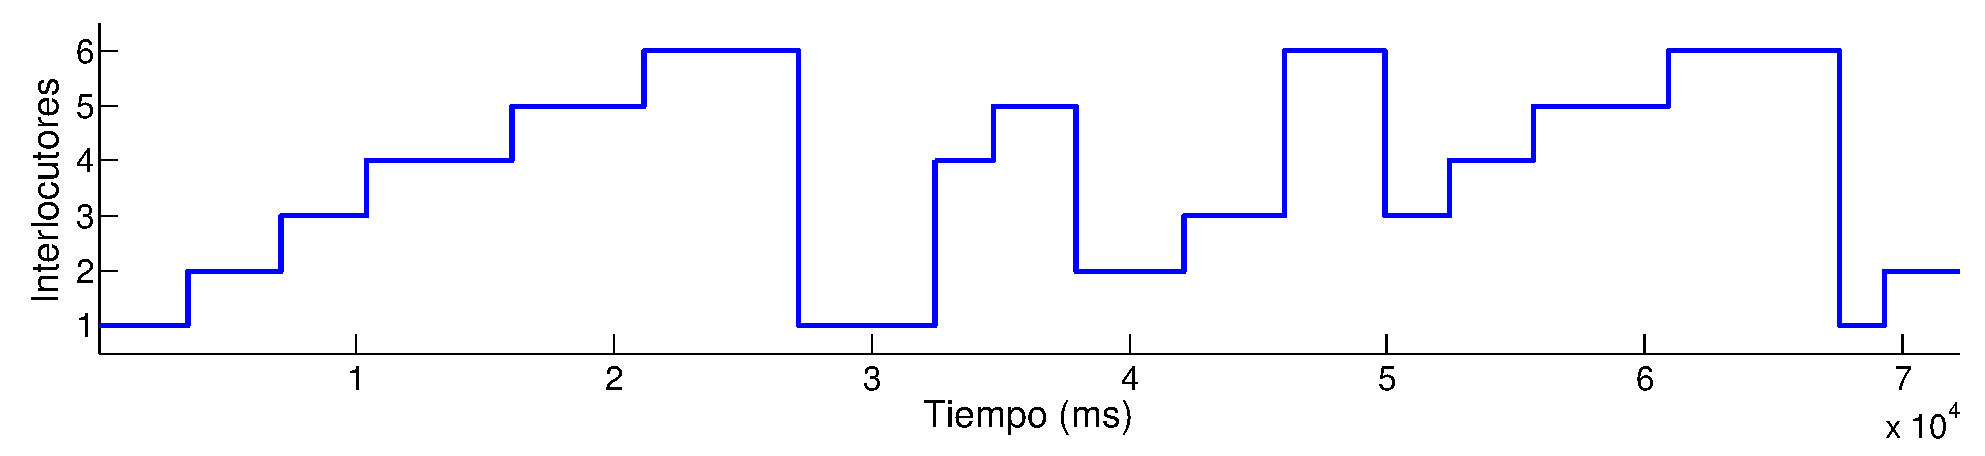
\includegraphics[width=1\linewidth]{gfx/chap6/cuervo1s_3_1}
      \caption{}
      \label{fig:seq1_seq1}
    \end{subfigure}
  } 
  \centerline
  {\begin{subfigure}[b]{1.3\textwidth}
      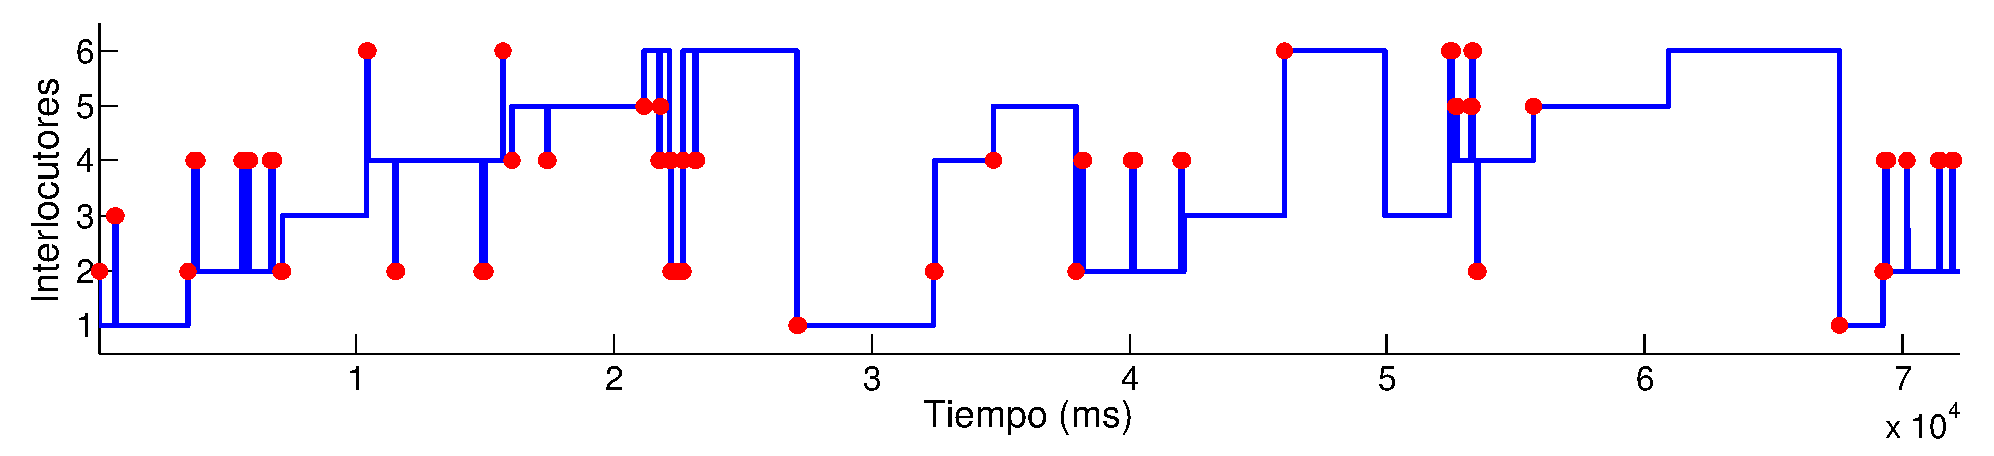
\includegraphics[width=1\linewidth]{gfx/chap6/cuervo1s_3_2}
      \caption{}
      \label{fig:seq1_seq2}
    \end{subfigure}
  }   
  \caption[Secuencia 1: Secuencia recuperada]{En \autoref{fig:seq1_seq1} se muestra la secuencia original de la \autoref{ssub:allanpoe}. En comparación, en \autoref{fig:seq1_seq2} se muestra la secuencia recuperada del modelo ganador y se marcan en rojo los errores cometidos respecto a la primera secuencia. }
  \label{fig:prb1_seq}
\end{figure}

Más a detalle, en la \autoref{fig:prb1_seq} se observa en azul el orden en el que participan los interlocutores de acuerdo a la secuencia recuperada. En rojo se marcan tanto los falsos positivos como los falsos negativos, de acuerdo al ground truth. 
Se observa también que la mayoría de las veces, en la secuencia recuperada se encuentran algunos brincos entre las personas, pero en esencia la estructura y el orden en que hablan los interlocutores es el correcto.
 

%%%%%%%%%%%%%%%%%%%%%%%%%%%%%%%%%%%%%%%%%%%%%%%%%%%%%%%%%%%%%%% 

\subsection[Secuencia 2]{Secuencia 2: Gabriel García Márquez} %(fold)
\label{ssub:soledad}

  Para la segunda secuencia se utilizaron algunos fragmentos de la novela 'El laberinto de la soledad' del escritor Gabriel García Márquez, con 4 distintas voces en español. La secuencia de audio original es de 6:55 min.

Para la etapa de agrupación de los vectores \ac{MFCC} con k-means++ se usaron 90 centros iniciales, mientras que el banco de filtros fue el mismo que en la secuencia anterior.

\begin{figure}[tp]
  \centerline{  
    \hspace{1.2cm}
    \parbox[c]{0.38\textwidth}{\centering Modelo generador}
    \parbox[c]{0.38\textwidth}{\centering Modelo $n_3$}
    \parbox[c]{0.38\textwidth}{\centering Modelo $n_4$}
    \parbox[c]{0.38\textwidth}{\centering Modelo $n_5$}
  }
  \vspace{0.5cm}
  \foreach \row in {1, ..., 2}{%  
    \centerline{%
      \parbox[c]{1cm}{
        \vspace{-0.5cm}
        \myheader{\row}
      }
      %\gdef \widthimg {0.35}
      \foreach \col in {1, ..., 4}{%
        \pgfmathparse{\col == 4 && \row == 2? 1:0}
        \ifthenelse{\pgfmathresult=1}{
          \gdef \widthimg {0.39}
        }{
          \gdef \widthimg {0.35}
        }
        \begin{subfigure}[c]{\widthimg \textwidth}          
          \def \imgfile {gfx/chap6/soledad1p_\col_\row}
          \IfFileExists{\imgfile.eps}{
            \includegraphics[width=1\textwidth]{\imgfile}
            \label{fig:seq2p_\col_\row}
          }{
            \hspace{1\textwidth}
          }
        \end{subfigure}
        %\hspace{-0.005\textwidth}
      }
    }
  }
\caption[Secuencia 2: Parámetros estimados (1)]{Por columnas, se muestran los parámetros obtenidos para varios modelos propuestos. La primer columna corresponde a los parámetros verdaderos.
En la primer fila \textup{(a)} se muestran las probabilidades a priori de que cada uno de los interlocutores empiecen la conversación. En la segunda fila \textup{(b)} se muestra en falso color la matriz de transición entre interlocutores para cada uno de los modelos mostrados.}
\label{fig:seq2p}
\end{figure}

En las \autoref{fig:seq2p} y \autoref{fig:seq2q} se muestran los parámetros estimados para los diferentes modelos que se propusieron. La primer columna corresponde a los parámetros verdaderos, mientras que las demás columnas son los parámetros obtenidos para diferentes modelos estimados. 

En la primer fila de la \autoref{fig:seq2p} se muestran las probabilidades a priori de que cada uno de los interlocutores empiecen el diálogo. En la segunda fila se muestra en falso color la matriz de transición para cada uno de los modelos. Esta matriz representa la probabilidad de cambio entre las personas que participan en la conversación.

De la misma manera, la matriz de transición que se recupera tiene estructura diagonal, como en la primer prueba.

\begin{figure}[t!]
  \centerline{
    \hspace{1.2cm}
    \parbox[c]{0.35\textwidth}{\centering Modelo generador}
    \parbox[c]{0.35\textwidth}{\centering Modelo $n_3$}
    \parbox[c]{0.35\textwidth}{\centering Modelo $n_4$}
    \parbox[c]{0.35\textwidth}{\centering Modelo $n_5$}
  }
  \vspace{0.5cm}
  \foreach \row in {3, ..., 7}{%  
    \centerline{
      \parbox[c]{1cm}{
        \vspace{-0.3cm}
        \myheader{\row}
      }
      \foreach \col in {1, ..., 4}{%
        \begin{subfigure}[c]{0.35\textwidth}  
          \def \imgfile {gfx/chap6/soledad1p_\col_\row}
          \IfFileExists{\imgfile.eps}{
            \includegraphics[width=1\textwidth]{\imgfile}
            %\caption{}
            \label{fig:seq2p_\col_\row}
          }{
            \hspace{1\textwidth}
          }
        \end{subfigure}
      }
    }
  }
\caption[Secuencia 2: Parámetros estimados (2)]{Por columnas, se muestran las probabilidades de emisión para cada uno de los interlocutores de acuerdo al modelo. Cada fila representa las probabilidad de emisión de las palabras en el diccionario. La fila \textup{(c)} para la primer persona, la fila \textup{(d)} para la segunda persona y así de forma consecutiva, de acuerdo al número de personas que contempla cada modelo propuesto.}
\label{fig:seq2q}
\end{figure}

En la \autoref{fig:seq2q} se muestran las probabilidades de emisión para cada uno de los participantes, de acuerdo a las palabras en las que se ha discretizado la conversación. Idealmente, cada interlocutor tiene asignadas con mayor probabilidad un cierto conjunto de palabras del diccionario, lo que hace que la identificación de las personas sea mucho más fácil de realizar.

Para la selección del modelo y como se explicó en el \autoref{ch:chap5}, primero se realiza una exploración del conjunto de posibles soluciones, por medio de \ac{BIC} regularizado para encontrar cuál o cuáles son los modelos más probables.

\begin{figure}[t!]
  \centerline{
  \begin{subfigure}[b]{1.1\textwidth}
   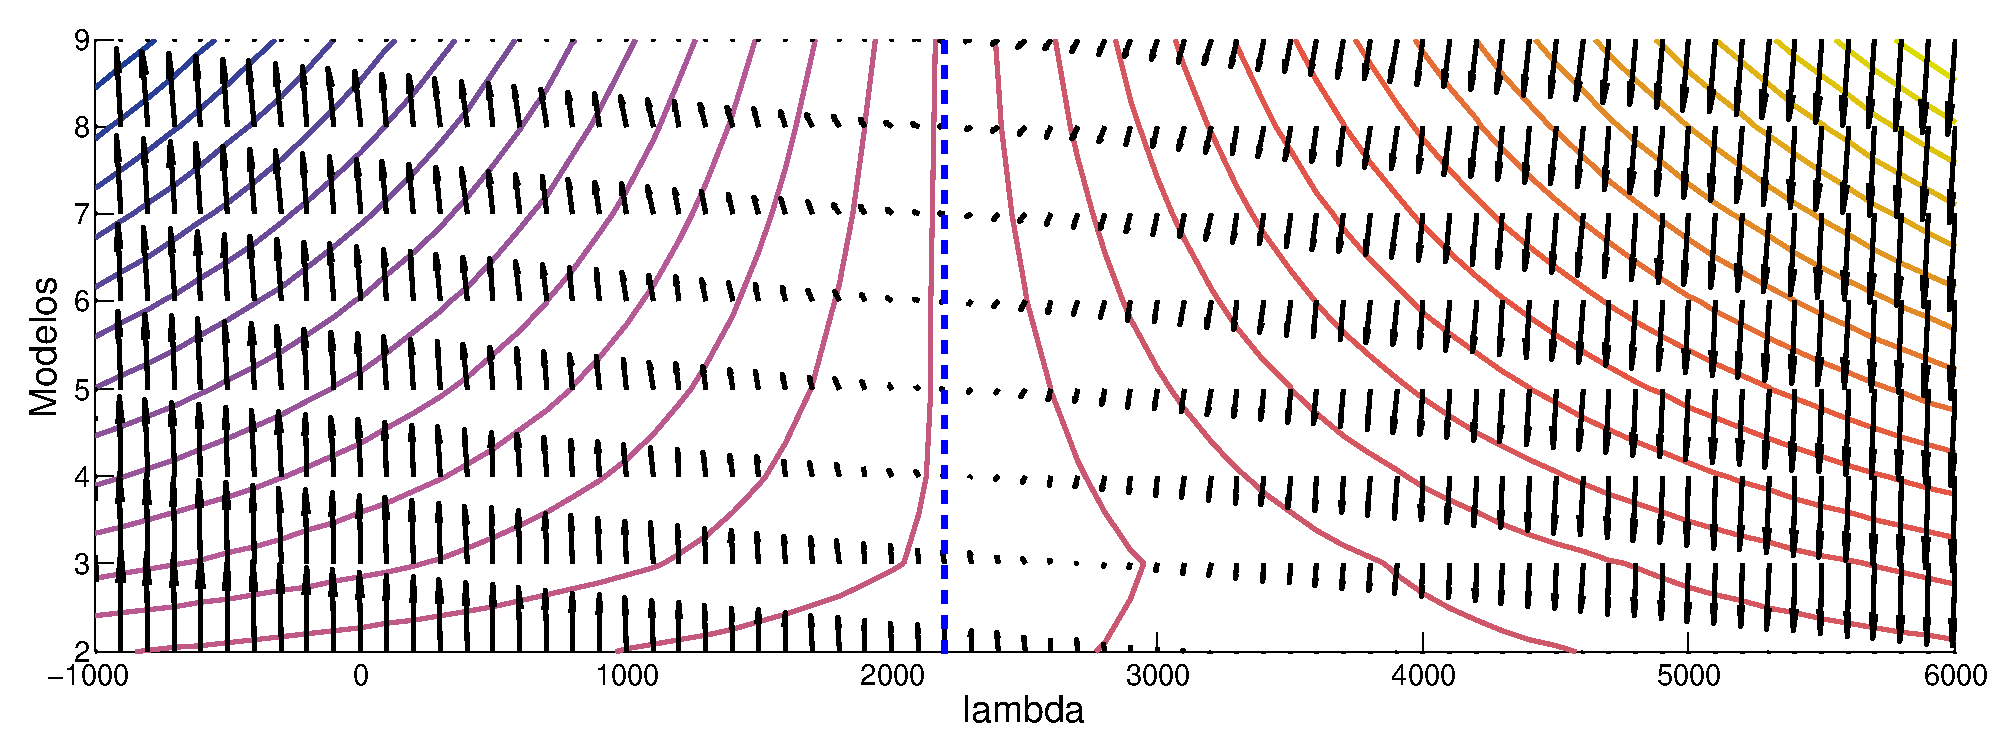
\includegraphics[width=1\textwidth]{gfx/chap6/calderon1bic2}
   \caption{}
   \label{fig:seq2_bic2}
  \end{subfigure}  
  }  
  \centerline{
  \begin{subfigure}[b]{0.55\textwidth}
    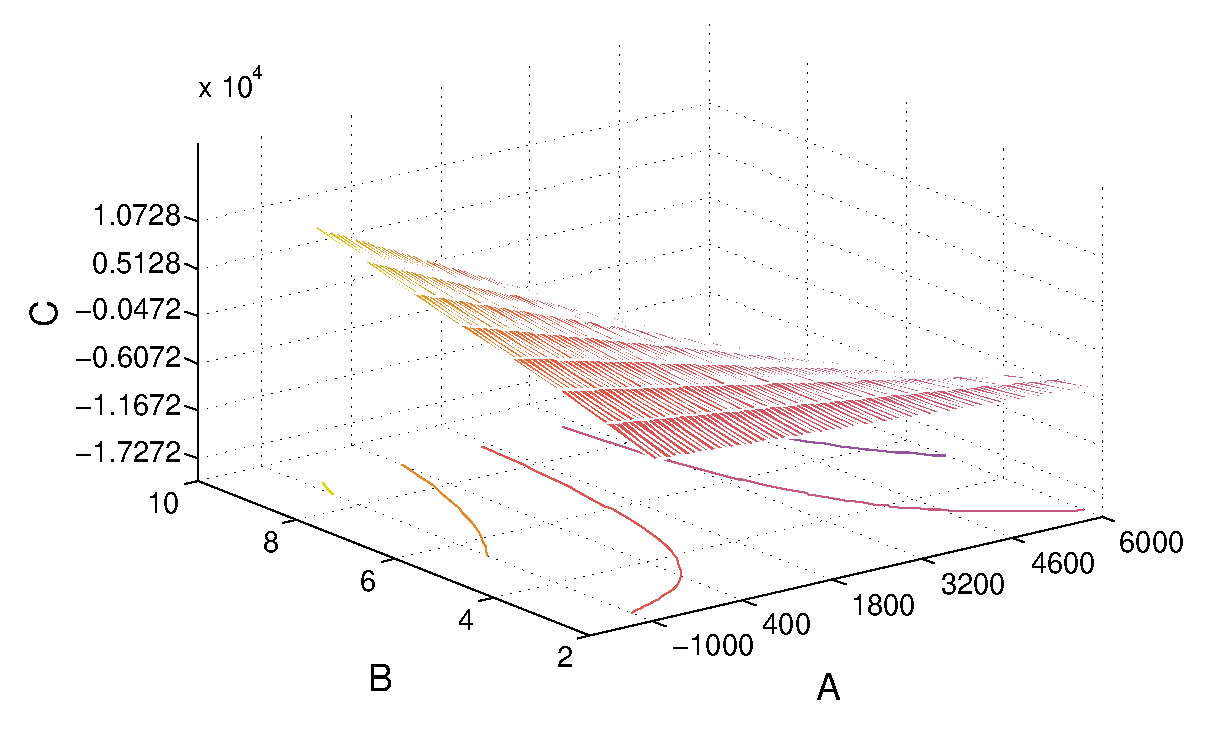
\includegraphics[width=\textwidth]{gfx/chap6/calderon1bic1} 
    \caption{}
    \label{fig:seq2_bic1}
  \end{subfigure}  
  \begin{subfigure}[b]{0.55\textwidth}
    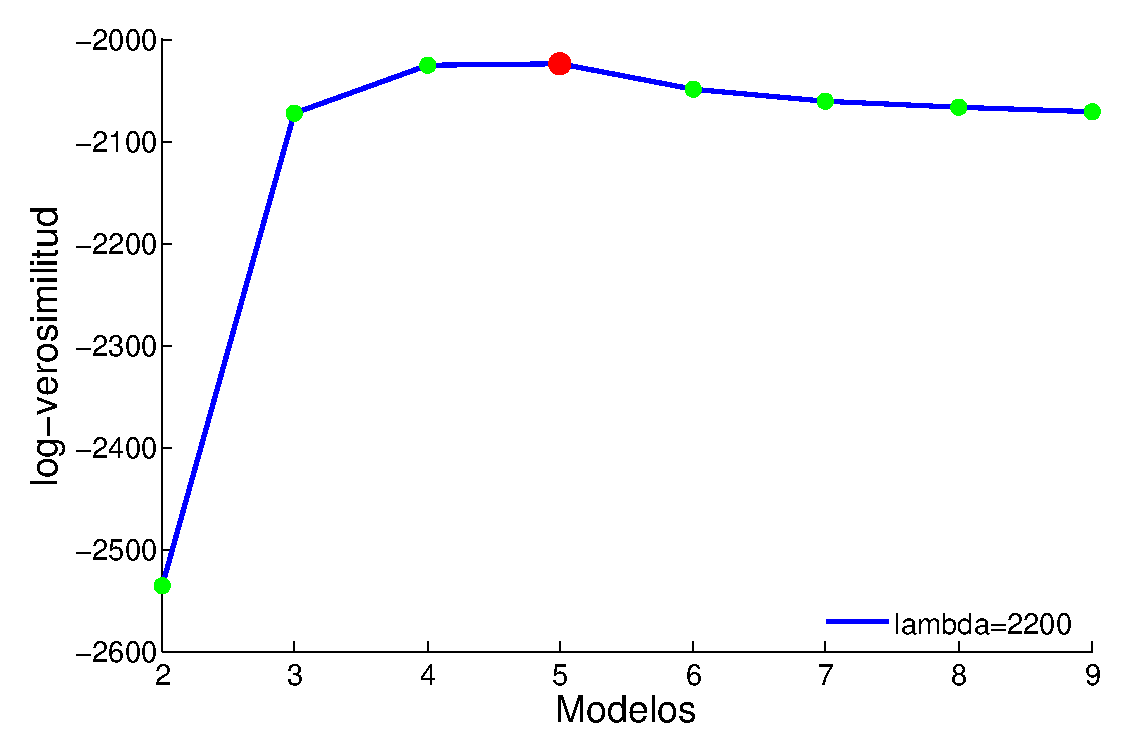
\includegraphics[width=\textwidth]{gfx/chap6/calderon1bic3} 
    \caption{}
    \label{fig:seq2_bic3}
  \end{subfigure}
  }
  \caption[Secuencia 2: Pruebas BIC]{En la \autoref{fig:seq2_bic2}, se muestra las curvas de nivel de la superficie al variar el valor de lambda para evaluar BIC, así como la dirección del gradiente en la misma. En la \autoref{fig:seq2_bic1} se muestra una perspectiva general de superficie en \autoref{fig:seq2_bic2}. En la \autoref{fig:seq2_bic3} se muestra el valor seleccionado para lambda de acuerdo al análisis de sensibilidad realizado en la superficie anterior.}
  \label{fig:seq2_bic}
\end{figure}

En la \autoref{fig:seq2_bic1} se muestra la superficie generada al variar el valor de $\lambda$ para diferentes curvas de selección \ac{BIC}. Haciendo un análisis de sensibilidad se puede determinar cuál es el parámetro $\lambda$ adecuado que penaliza de buena forma la log-verosimilitud. En la \autoref{fig:seq2_bic2} se muestran las curvas de nivel de la figura anterior, además de la dirección del gradiente de la misma. Así mismo, en falso color se resaltan las zonas en las que el gradiente es menor. 

Por último, se muestra en \autoref{fig:seq2_bic3} la curva \ac{BIC} con el valor de $\lambda$ encontrado a partir del análisis de sensibilidad realizado en la \autoref{fig:seq2_bic2}. El o los modelos que tengan un mayor valor \ac{BIC} serán los que se seleccionarán como modelos ganadores.

\begin{figure}[t!]
  \centerline  
  { \begin{subfigure}[b]{0.7\textwidth}
      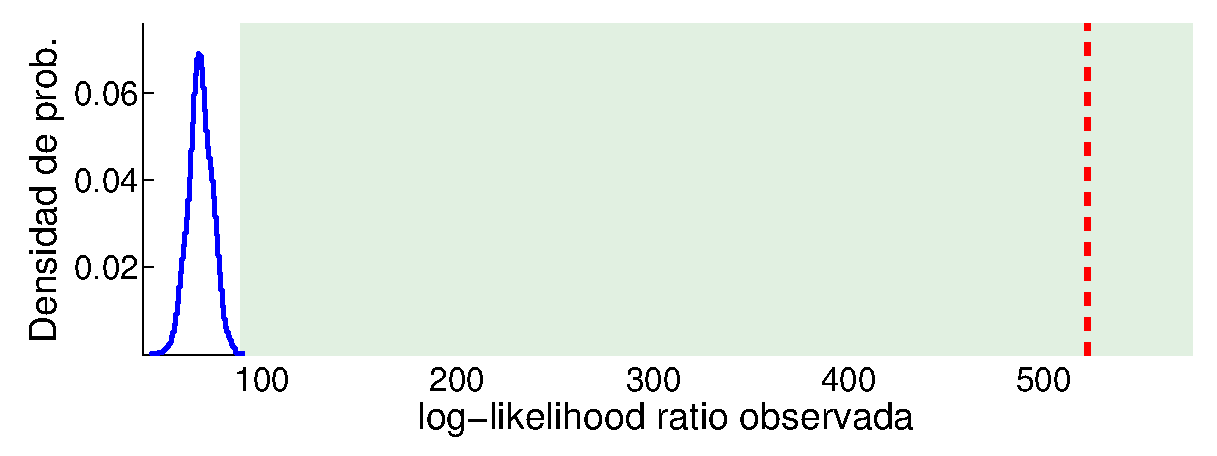
\includegraphics[width=1\linewidth]{gfx/chap6/soledad1boot1}
      \caption{}
      \label{fig:seq2_boot1}
    \end{subfigure}
    \hspace{0.5cm}
    \begin{subfigure}[b]{0.7\textwidth}
      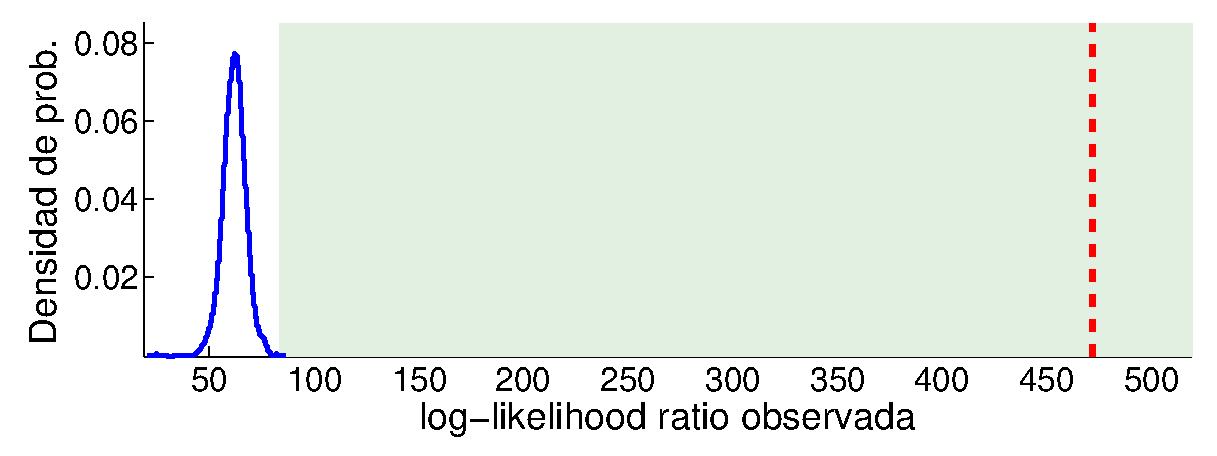
\includegraphics[width=1\linewidth]{gfx/chap6/soledad1boot2}
      \caption{}
      \label{fig:seq2_boot2}
    \end{subfigure}
  }
  \centerline  
  { \begin{subfigure}[b]{0.7\textwidth}
      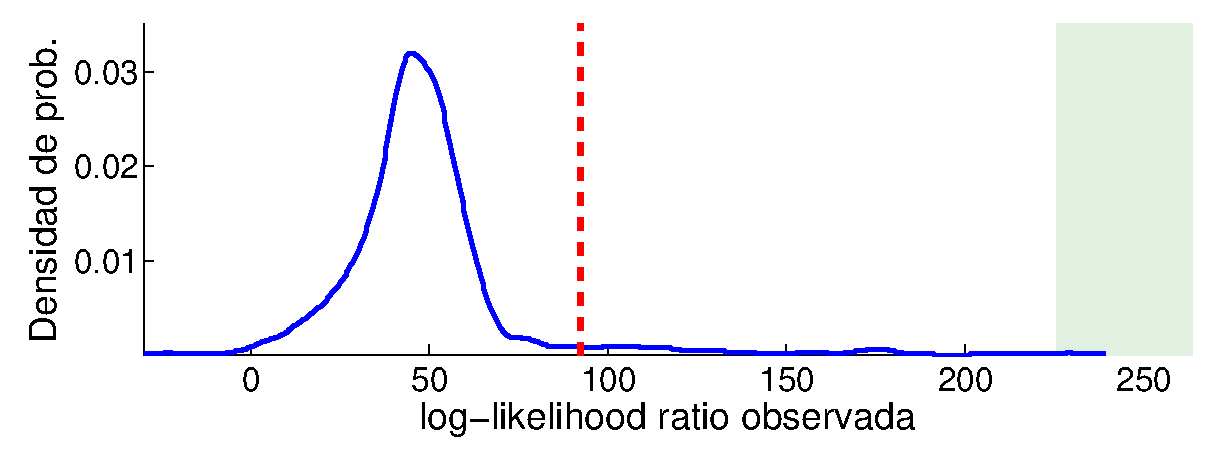
\includegraphics[width=1\linewidth]{gfx/chap6/soledad1boot3}
      \caption{}
      \label{fig:seq2_boot3}
    \end{subfigure}
    \hspace{0.5cm}
    \begin{subfigure}[b]{0.7\textwidth}
      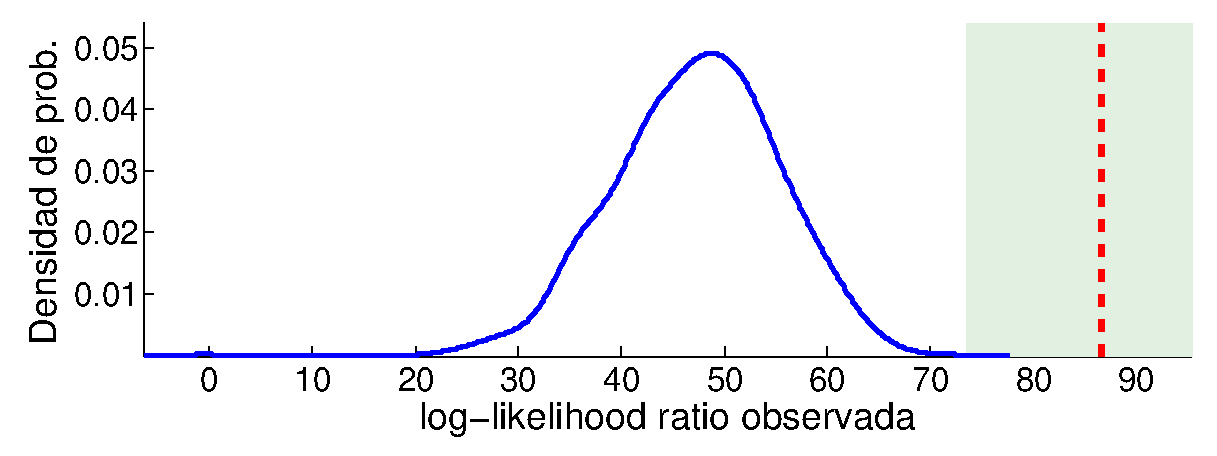
\includegraphics[width=1\linewidth]{gfx/chap6/soledad1boot4}
      \caption{}
      \label{fig:seq2_boot4}
    \end{subfigure}
  }
  \caption[Secuencia 2: Pruebas de hipótesis usando bootstrap]{En la \autoref{fig:seq2_boot1} se muestra la prueba de hipótesis realizada para comparar el modelo $n_2$ contra $n_3$. Como se observa, se rechaza la hipótesis de que el modelo correcto sea $n_4$. En la \autoref{fig:seq2_boot2} se hace la prueba del modelo $n_3$ contra $n_4$, y de la misma manera, se rechaza la hipótesis de que el modelo correcto sea $n_3$. Se sigue con la prueba de hipótesis del modelo $n_4$ contra $n_5$ en la \autoref{fig:seq2_boot3}, y en este caso el valor observado no cae dentro de la región de rechazo, por lo que no podemos rechazar que el modelo $n_4$ sea el correcto. Por último en la \autoref{fig:seq2_boot4}, se hace la prueba del modelo $n_5$ contra el modelo $n_6$, y se vuelve a rechazar la hipótesis nula.}  
  \label{fig:seq2_boot}
\end{figure}

En caso de que después de utilizar BIC se presente ambigüedad para determinar un modelo ganador, o ya sea para realizar un análisis más exhaustivo, se puede propone hacer una prueba de hipótesis para determinar cuál modelo se ajusta mejor a los datos.

A diferencia de la primer etapa, en la que se usa BIC como criterio para  seleccionar el mejor modelo de un conjunto no definido de modelos con diferentes parámetros, la intención de hacer pruebas de hipótesis es determinar en un pequeño conjunto de probables modelos, cuál es mejor, y qué tan bueno es un modelo respecto a otro.

Al plantear la prueba de hipótesis se harán una gran cantidad de simulaciones para ver qué tan bien se ajusta cada modelo a los datos originales, por lo que este proceso es computacionalmente intensivo y sólo se recomienda hacerlo para evitar la ambigüedad entre un par de modelos.

...

Por último, ya con el modelo seleccionado, se procede a calcular el error relativo de predicción que se obtuvo, comparando con el ground truth que se dispone para esa secuencia, con lo que se obtiene: 

...

\begin{figure}[tp]
  \centerline
  {\begin{subfigure}[b]{1.3\textwidth}
      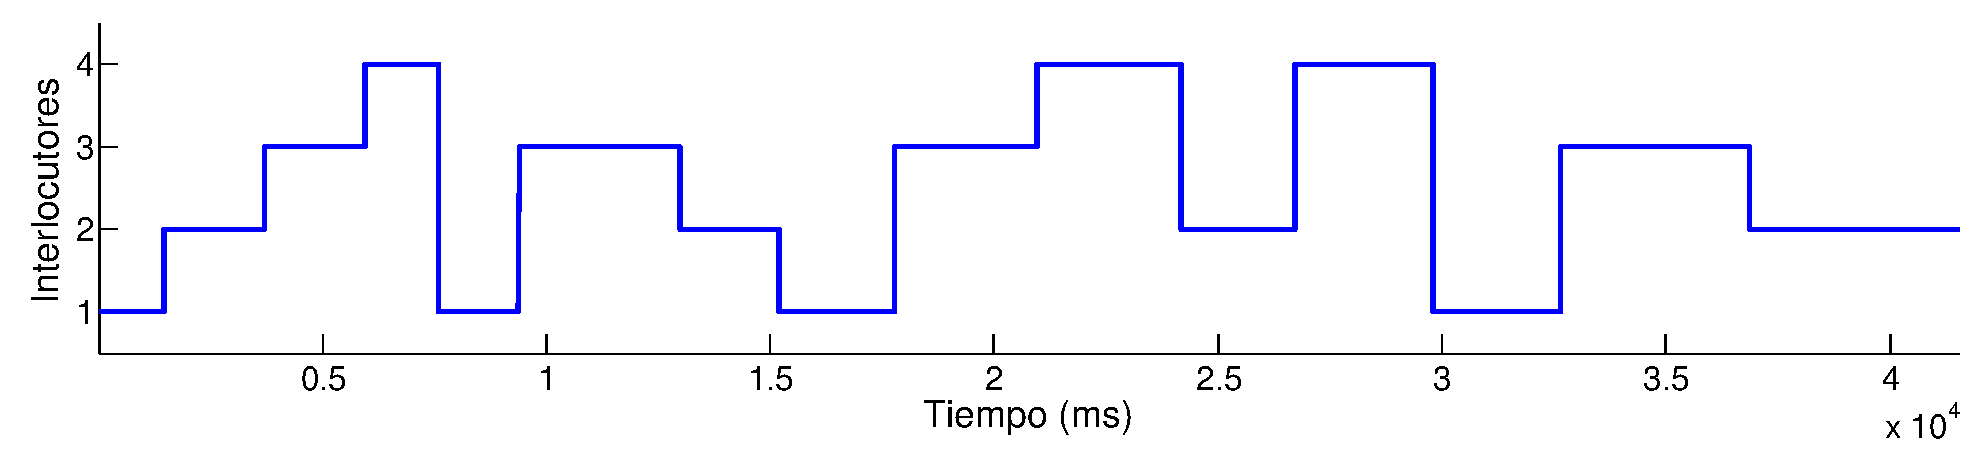
\includegraphics[width=1\linewidth]{gfx/chap6/soledad1s_3_1}
      \caption{}
      \label{fig:seq2_seq1}
    \end{subfigure}
  } 
  \centerline
  {\begin{subfigure}[b]{1.3\textwidth}
      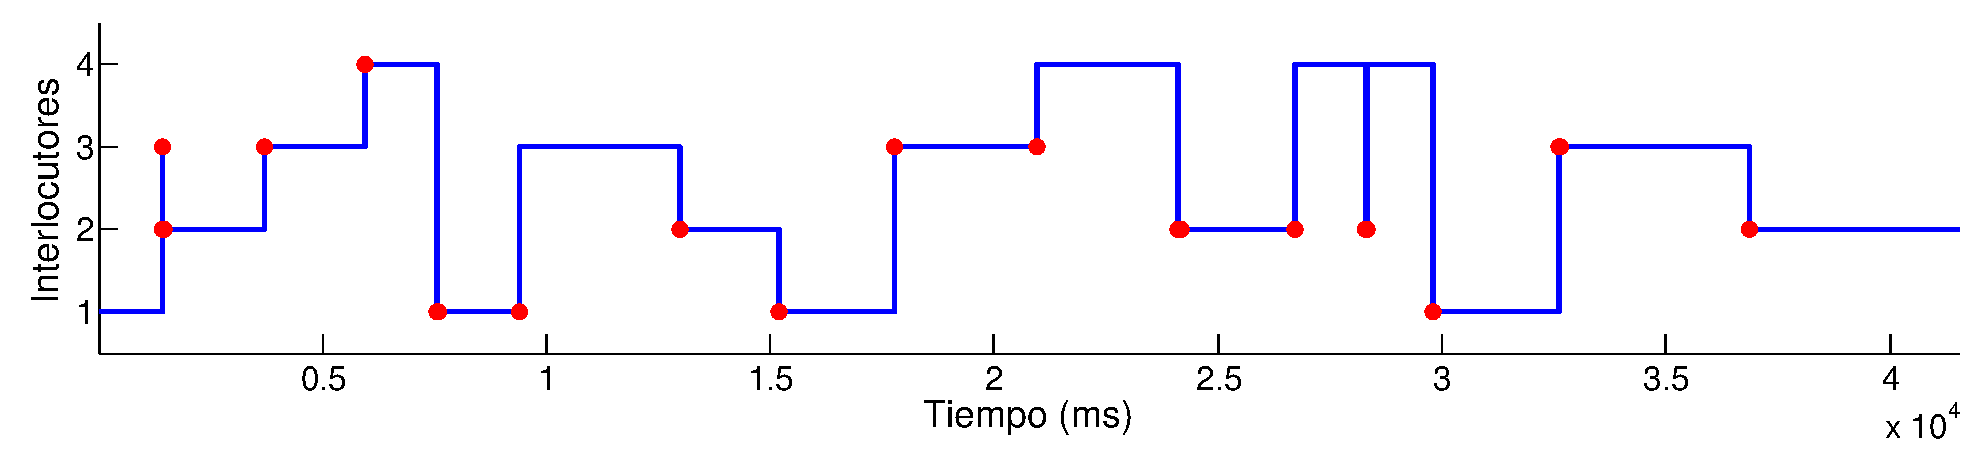
\includegraphics[width=1\linewidth]{gfx/chap6/soledad1s_3_2}
      \caption{}
      \label{fig:seq2_seq2}
    \end{subfigure}
  }
  \caption[Secuencia 2: Secuencia recuperada]{En \autoref{fig:seq2_seq1} se muestra la secuencia original de la \autoref{ssub:soledad}. En comparación, en \autoref{fig:seq2_seq2} se muestra la secuencia recuperada del modelo ganador y se marcan en rojo los errores cometidos respecto a la primera secuencia. }
  \label{fig:prb2_seq}
\end{figure}

Más a detalle, en la \autoref{fig:prb2_seq} se observa en azul el orden en el que participan los interlocutores de acuerdo a la secuencia recuperada. En rojo se marcan tanto los falsos positivos como los falsos negativos, de acuerdo al ground truth. Hay que notar que cuando el número de estados para un modelo no es el correcto, entonces inminentemente el número de errores en la secuencia obtenida será mayor, pues al menos todas las intervenciones de un hablante no podrán ser emparejadas o serán asignadas a alguien más.

Se observa también que la mayoría de las veces, en la secuencia recuperada se encuentran algunos brincos entre personas, pero en esencia la estructura y el orden en que hablan los interlocutores es el correcto. 

%%%%%%%%%%%%%%%%%%%%%%%%%%%%%%%%%%%%%%%%%%%%%%%%%%%%%%%%%%%%%%% 

\subsection[Secuencia 3]{Secuencia 3: William Shakespeare}
\label{ssub:lear}

  Para esta secuencia se utilizaron algunos poemas del escritor William Shakespeare, alternando 6 voces diferentes en inglés. La secuencia de audio original tiene una duración de 12:01 min.

Para la etapa de agrupación de los vectores MFCC con k-means++ se usaron 140 centros iniciales, mientras que el banco de filtros fue el mismo que en la secuencia anterior.

\begin{figure}[tp]
  \centerline{  
    \hspace{1.2cm}
    \parbox[c]{0.38\textwidth}{\centering Modelo generador}
    \parbox[c]{0.38\textwidth}{\centering Modelo $n_5$}
    \parbox[c]{0.38\textwidth}{\centering Modelo $n_6$}
    \parbox[c]{0.38\textwidth}{\centering Modelo $n_7$}
  }
  \vspace{0.5cm}
  \foreach \row in {1, ..., 2}{%  
    \centerline{%
      \parbox[c]{1cm}{
        \vspace{-0.5cm}
        \myheader{\row}
      }
      %\gdef \widthimg {0.35}
      \foreach \col in {1, ..., 4}{%
        \pgfmathparse{\col == 4 && \row == 2? 1:0}
        \ifthenelse{\pgfmathresult=1}{
          \gdef \widthimg {0.39}
        }{
          \gdef \widthimg {0.35}
        }
        \begin{subfigure}[c]{\widthimg \textwidth}          
          \def \imgfile {gfx/chap6/lear3p_\col_\row}
          \IfFileExists{\imgfile.eps}{
            \includegraphics[width=1\textwidth]{\imgfile}
            \label{fig:seq3p_\col_\row}
          }{
            \hspace{1\textwidth}
          }
        \end{subfigure}
        %\hspace{-0.005\textwidth}
      }
    }
  }
\caption[Secuencia 3: Parámetros estimados (1)]{Por columnas, se muestran los parámetros obtenidos para varios modelos propuestos. La primer columna corresponde a los parámetros verdaderos.
En la primer fila \textup{(a)} se muestran las probabilidades a priori de que cada uno de los interlocutores empiecen la conversación. En la segunda fila \textup{(b)} se muestra en falso color la matriz de transición entre interlocutores para cada uno de los modelos mostrados.}
\label{fig:seq3p}
\end{figure}

En las \autoref{fig:seq3p} y \autoref{fig:seq3q} se muestran los parámetros estimados para los diferentes modelos que se propusieron. La primer columna corresponde a los parámetros verdaderos, mientras que las demás columnas son los parámetros obtenidos para diferentes modelos estimados. 

En la primer fila de la \autoref{fig:seq3p} se muestran las probabilidades a priori de que cada uno de los interlocutores empiecen el diálogo. En la segunda fila se muestra en falso color la matriz de transición para cada uno de los modelos. Esta matriz representa la probabilidad de cambio entre las personas que participan en la conversación.

Se observa como en general para todos los modelos propuestos la matriz de transición que se recupera tiene una estructura diagonal, puesto que en este tipo de problemas, una persona suele hablar durante un periodo considerablemente largo, para que luego otra persona empiece a hablar.

\begin{figure}[t!]
  \centerline{
    \hspace{1.2cm}
    \parbox[c]{0.35\textwidth}{\centering Modelo generador}
    \parbox[c]{0.35\textwidth}{\centering Modelo $n_5$}
    \parbox[c]{0.35\textwidth}{\centering Modelo $n_6$}
    \parbox[c]{0.35\textwidth}{\centering Modelo $n_7$}
  }
  \vspace{0.5cm}
  \foreach \row in {3, ..., 7}{%  
    \centerline{
      \parbox[c]{1cm}{
        \vspace{-0.3cm}
        \myheader{\row}
      }
      \foreach \col in {1, ..., 4}{%
        \begin{subfigure}[c]{0.35\textwidth}  
          \def \imgfile {gfx/chap6/lear3p_\col_\row}
          \IfFileExists{\imgfile.eps}{
            \includegraphics[width=1\textwidth]{\imgfile}
            %\caption{}
            \label{fig:seq3p_\col_\row}
          }{
            \hspace{1\textwidth}
          }
        \end{subfigure}
      }
    }
  }
\caption[Secuencia 3: Parámetros estimados (2)]{Por columnas, se muestran las probabilidades de emisión para cada uno de los interlocutores de acuerdo al modelo. Cada fila representa las probabilidad de emisión de las palabras en el diccionario. La fila \textup{(c)} para la primer persona, la fila \textup{(d)} para la segunda persona y así de forma consecutiva, de acuerdo al número de personas que contempla cada modelo propuesto.}
\label{fig:seq3q}
\end{figure}

En la \autoref{fig:seq3q} se muestran las probabilidades de emisión para cada uno de los participantes, de acuerdo a las palabras en las que se ha discretizado la conversación. Idealmente, cada interlocutor tiene asignadas con mayor probabilidad un cierto conjunto de palabras del diccionario, lo que hace que la identificación de las personas sea mucho más fácil de realizar.

Para la selección del modelo y siguiendo la metodología propuesta, primero se efectúa una inspección por medio de BIC regularizado para encontrar cuál o cuáles son los modelos más probables.

\begin{figure}[t!]
  \centerline{
  \begin{subfigure}[b]{1.1\textwidth}
   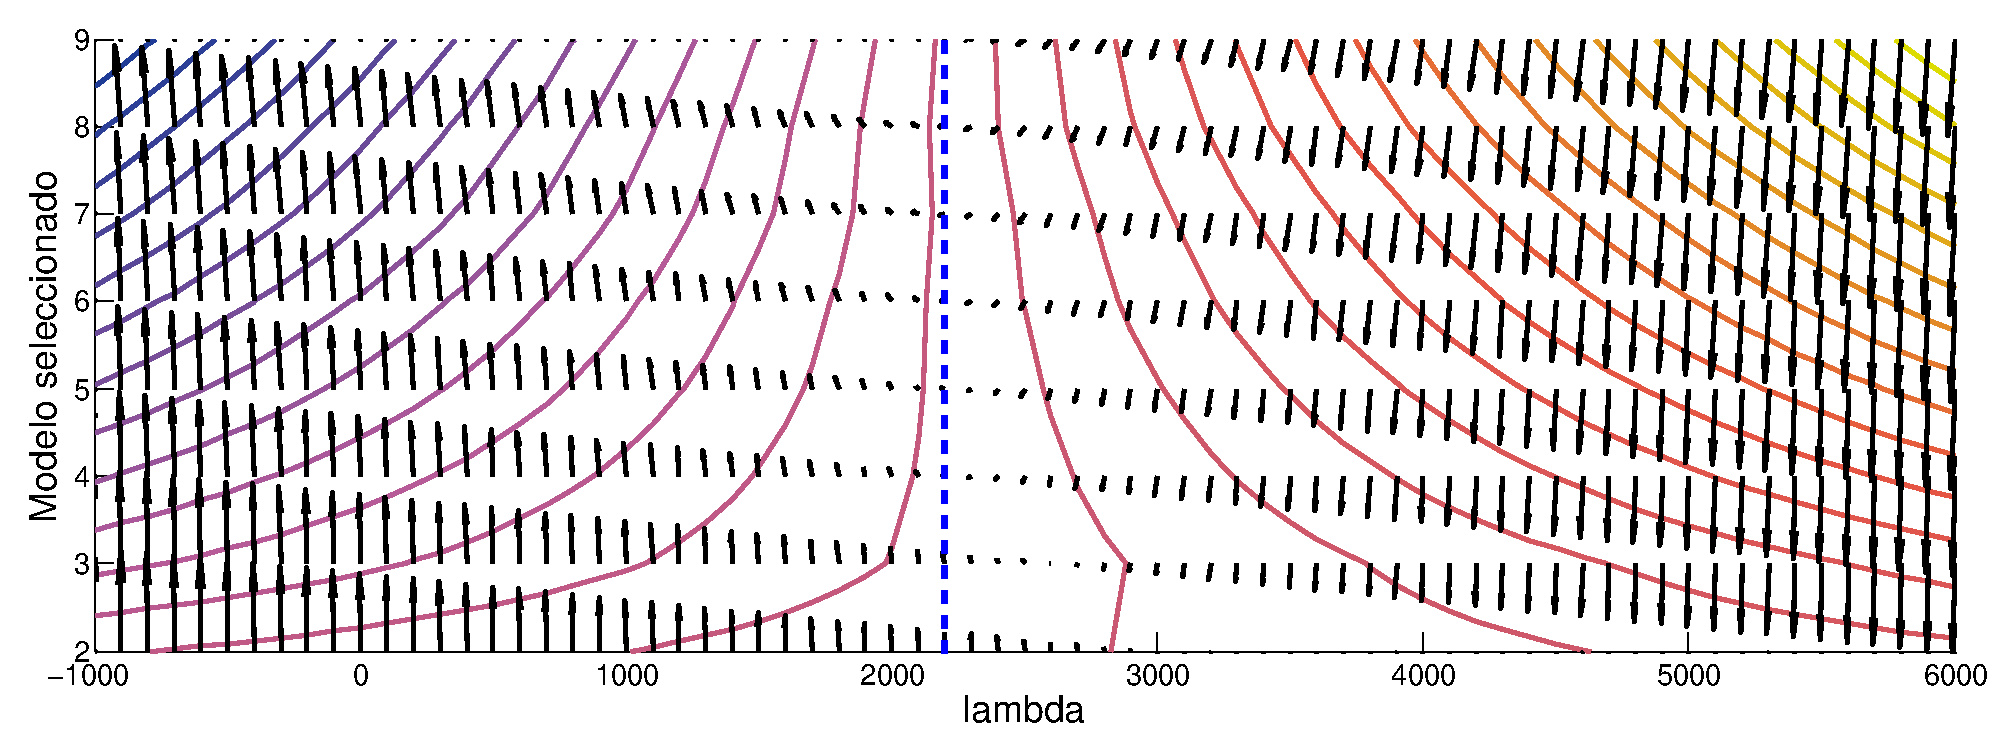
\includegraphics[width=1\textwidth]{gfx/chap6/lear3bic2}
   \caption{}
   \label{fig:seq3_bic2}
  \end{subfigure}  
  }  
  \centerline{
  \begin{subfigure}[b]{0.55\textwidth}
    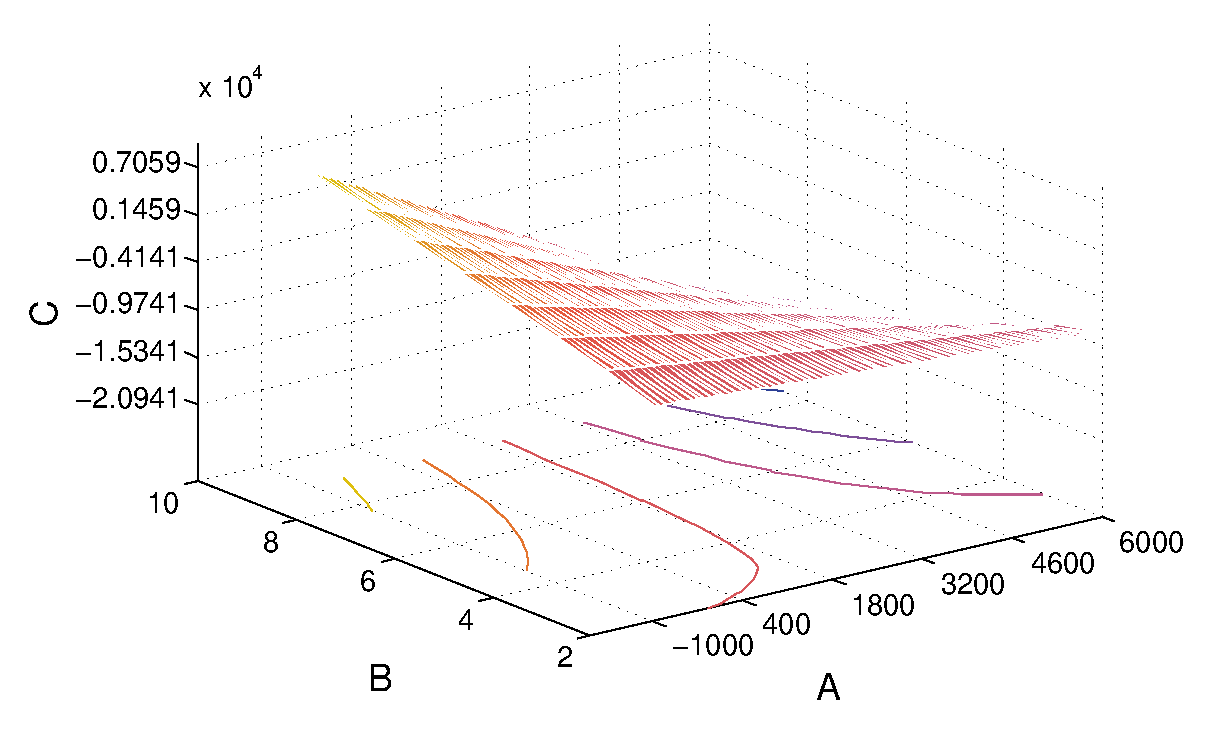
\includegraphics[width=\textwidth]{gfx/chap6/lear3bic1} 
    \caption{}
    \label{fig:seq3_bic1}
  \end{subfigure}  
  \begin{subfigure}[b]{0.55\textwidth}
    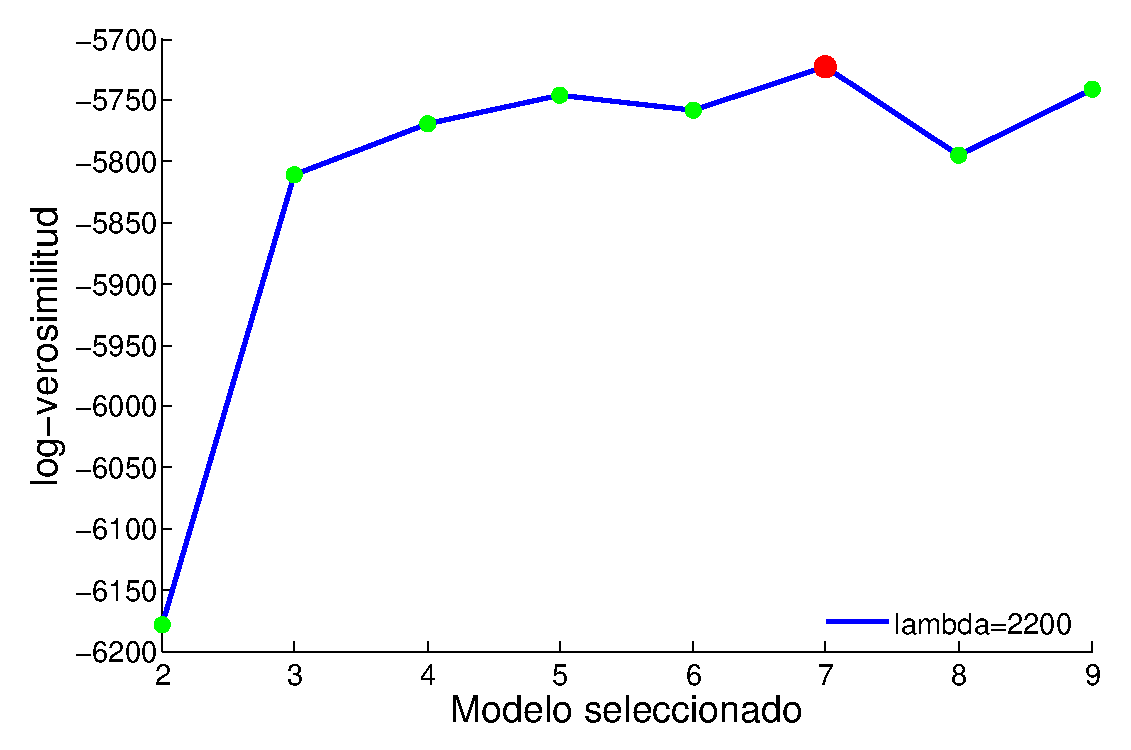
\includegraphics[width=\textwidth]{gfx/chap6/lear3bic3} 
    \caption{}
    \label{fig:seq3_bic3}
  \end{subfigure}
  }
  \caption[Secuencia 3: Pruebas BIC]{En la \autoref{fig:seq3_bic2}, se muestra las curvas de nivel de la superficie al variar el valor de lambda para evaluar BIC, así como la dirección del gradiente en la misma. En la \autoref{fig:seq3_bic1} se muestra una perspectiva general de superficie en \autoref{fig:seq3_bic2}. En la \autoref{fig:seq3_bic3} se muestra el valor seleccionado para lambda de acuerdo al análisis de sensibilidad realizado en la superficie anterior.}
  \label{fig:seq1_bic}
\end{figure}

En la \autoref{fig:seq3_bic1} se muestra la superficie generada al variar el valor de $\lambda$ para diferentes curvas de selección BIC. Se observa cómo al principio $\lambda$ es muy pequeño, y entonces el término de penalización no funciona por lo que se prefieren los modelos más complejos y sobre ajustados. Por otro lado, cuando $\lambda$ es muy grande, la penalización no permite mas que escoger los modelos más simples.

Haciendo un análisis de sensibilidad se puede determinar cuál es el parámetro $\lambda$ adecuado que penaliza de buena forma la log-verosimilitud.

En la \autoref{fig:seq3_bic2} se muestran las curvas de nivel de la figura anterior, además de la dirección del gradiente de la misma. Así mismo, en falso color se resaltan las zonas en las que el gradiente es menor. 

Lo que nos interesa encontrar en la superficie, es el valor de $\lambda$ que representa el punto de inflexión entre la selección de modelos demasiado complejos y modelos más simples. Para esto, se busca la zona en la que el gradiente sea lo más cercano a cero, pues implicaría que es un punto crítico.

Debido a la escala y a la forma en la que se calculó el gradiente, aunque para algunos valores cercanos de $\lambda$ no haya mucha variación en esa dirección; si BIC está penalizando mal, entonces sí habrá gran variación para los diferentes modelos. Es por esto, que sólo en la zona en que la penalización sea del mismo orden de magnitud que la verosimilitud la variación en la curva BIC con el $\lambda$ adecuado no será tan grande como en otras zonas.

Por último, se muestra en \autoref{fig:seq3_bic3} la curva BIC con el valor de $\lambda$ encontrado a partir del análisis de sensibilidad realizado en la \autoref{fig:seq3_bic2}. El o los modelos que tengan un mayor valor BIC serán los que se seleccionarán como modelos ganadores.

\begin{figure}[t!]
  \centerline  
  { \begin{subfigure}[b]{0.7\textwidth}
      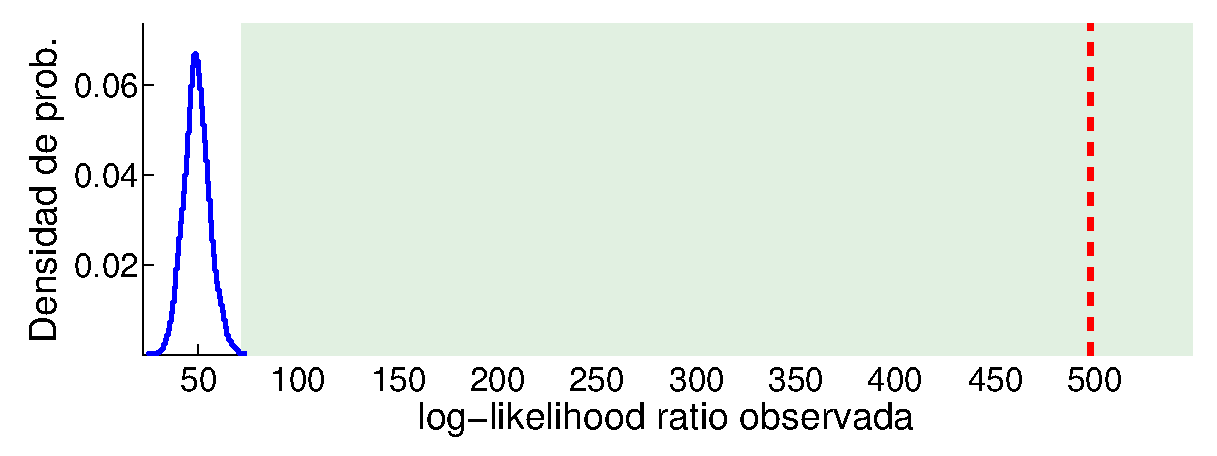
\includegraphics[width=1\linewidth]{gfx/chap6/lear3boot1}
      \caption{}
      \label{fig:seq3_boot1}
    \end{subfigure}
    \hspace{0.5cm}
    \begin{subfigure}[b]{0.7\textwidth}
      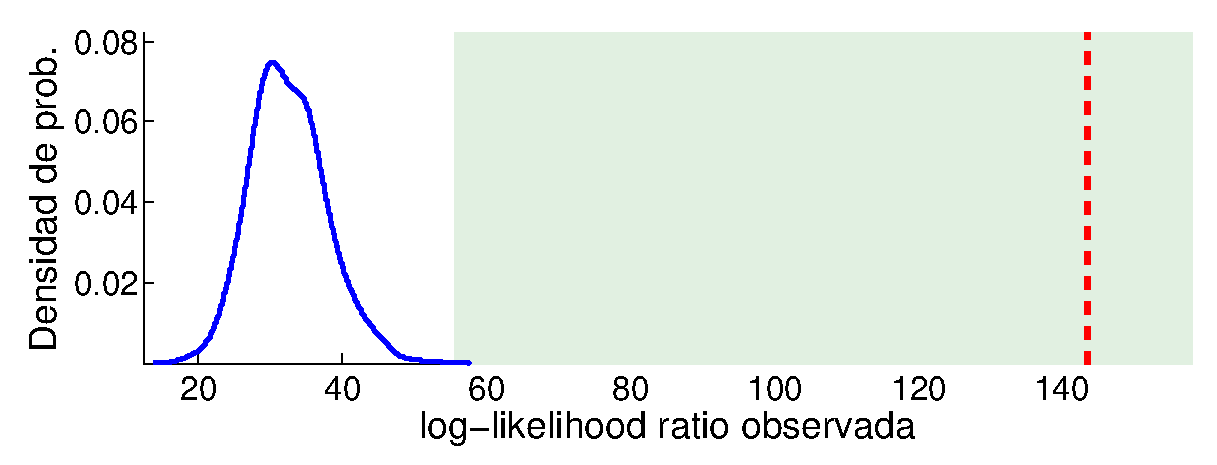
\includegraphics[width=1\linewidth]{gfx/chap6/lear3boot2}
      \caption{}
      \label{fig:seq3_boot2}
    \end{subfigure}
  }
  \centerline  
  { \begin{subfigure}[b]{0.7\textwidth}
      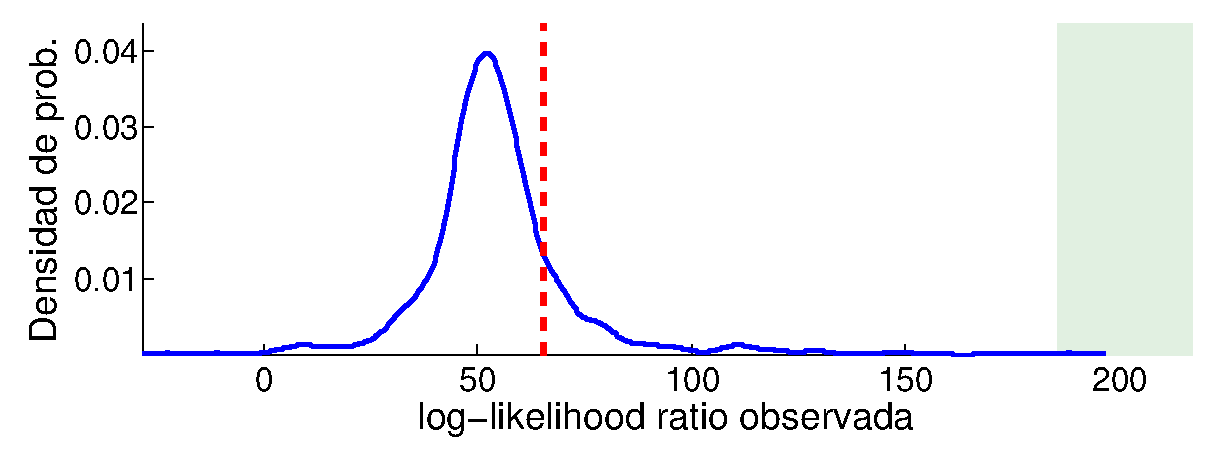
\includegraphics[width=1\linewidth]{gfx/chap6/lear3boot3}
      \caption{}
      \label{fig:seq3_boot3}
    \end{subfigure}
    \hspace{0.5cm}
    \begin{subfigure}[b]{0.7\textwidth}
      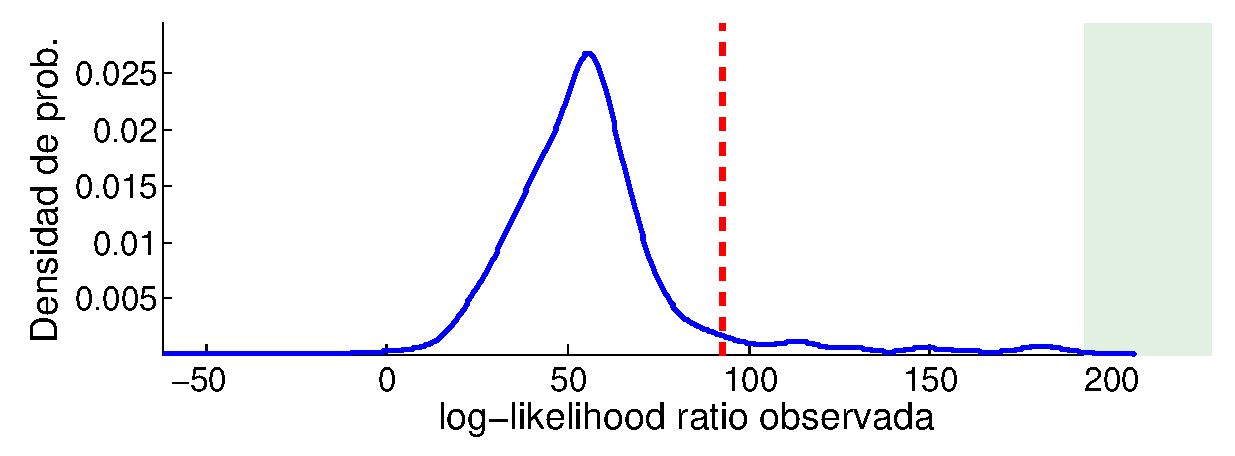
\includegraphics[width=1\linewidth]{gfx/chap6/lear3boot4}
      \caption{}
      \label{fig:seq3_boot4}
    \end{subfigure}
  }
  \caption[Secuencia 3: Pruebas de hipótesis usando bootstrap]{En la \autoref{fig:seq3_boot1} se muestra la prueba de hipótesis realizada para comparar el modelo $n_4$ contra $n_5$. Como se observa, se rechaza la hipótesis de que el modelo correcto sea $n_4$. En la \autoref{fig:seq3_boot2} se hace la prueba del modelo $n_5$ contra $n_6$, y de la misma manera, se rechaza la hipótesis de que el modelo correcto sea $n_5$. Se sigue con la prueba de hipótesis del modelo $n_6$ contra $n_7$ en la \autoref{fig:seq3_boot3}, y en este caso el valor observado no cae dentro de la región de rechazo, por lo que no podemos rechazar que el modelo $n_6$ sea el correcto. Por último en la \autoref{fig:seq3_boot4}, se hace la prueba del modelo $n_7$ contra el modelo $n_8$, y se vuelve a rechazar la hipótesis nula.}  
  \label{fig:seq3_boot}
\end{figure}

En caso de que después de utilizar BIC se presente ambigüedad para determinar un modelo ganador, o ya sea para realizar un análisis más exhaustivo, se puede propone hacer una prueba de hipótesis para determinar cuál modelo se ajusta mejor a los datos.

A diferencia de la primer etapa, en la que se usa BIC como criterio para  seleccionar el mejor modelo de un conjunto no definido de modelos con diferentes parámetros, la intención de hacer pruebas de hipótesis es determinar en un pequeño conjunto de probables modelos, cuál es mejor, y qué tan bueno es un modelo respecto a otro.

Al plantear la prueba de hipótesis se harán una gran cantidad de simulaciones para ver qué tan bien se ajusta cada modelo a los datos originales, por lo que este proceso es computacionalmente intensivo y sólo se recomienda hacerlo para evitar la ambigüedad entre un par de modelos.

...

Por último, ya con el modelo seleccionado, se procede a calcular el error relativo de predicción que se obtuvo, comparando con el ground truth que se dispone para esa secuencia, con lo que se obtiene: 

...

\begin{figure}[tp]
  \centerline
  {\begin{subfigure}[b]{1.3\textwidth}
      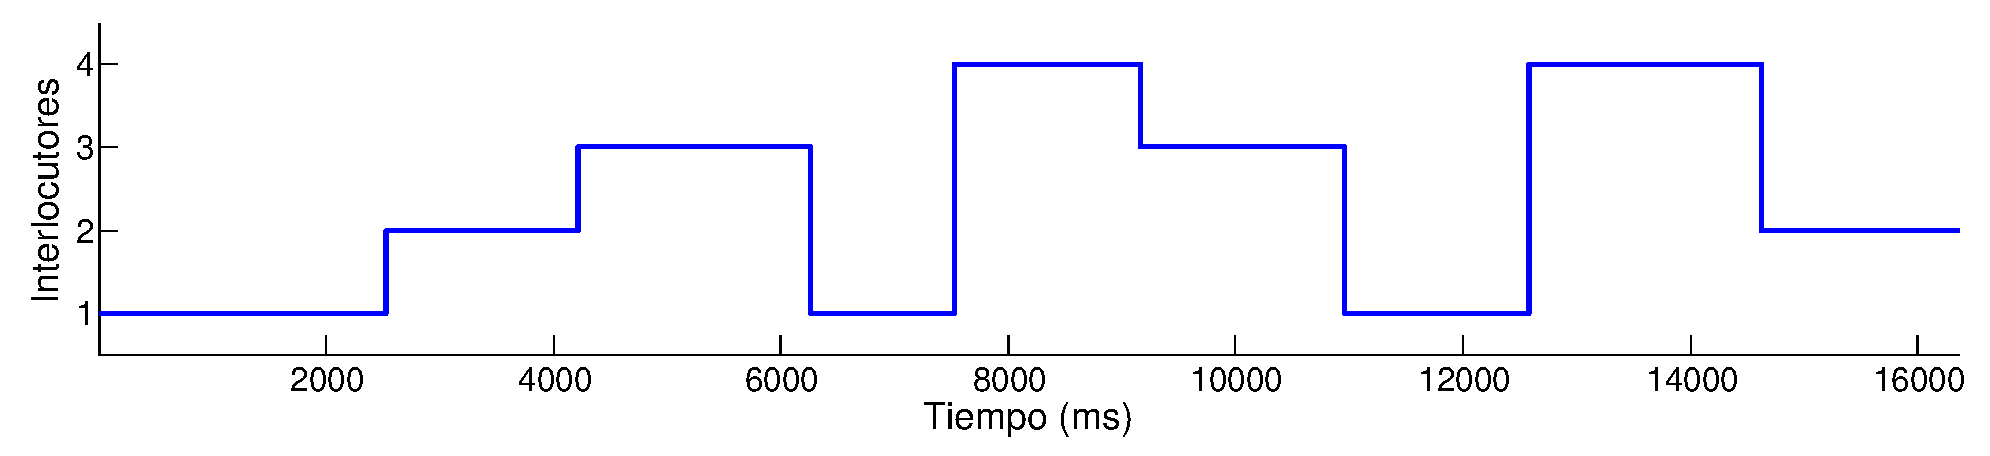
\includegraphics[width=1\linewidth]{gfx/chap6/lear3s_3_1}
      \caption{}
      \label{fig:seq3_seq1}
    \end{subfigure}
  } 
  \centerline
  {\begin{subfigure}[b]{1.3\textwidth}
      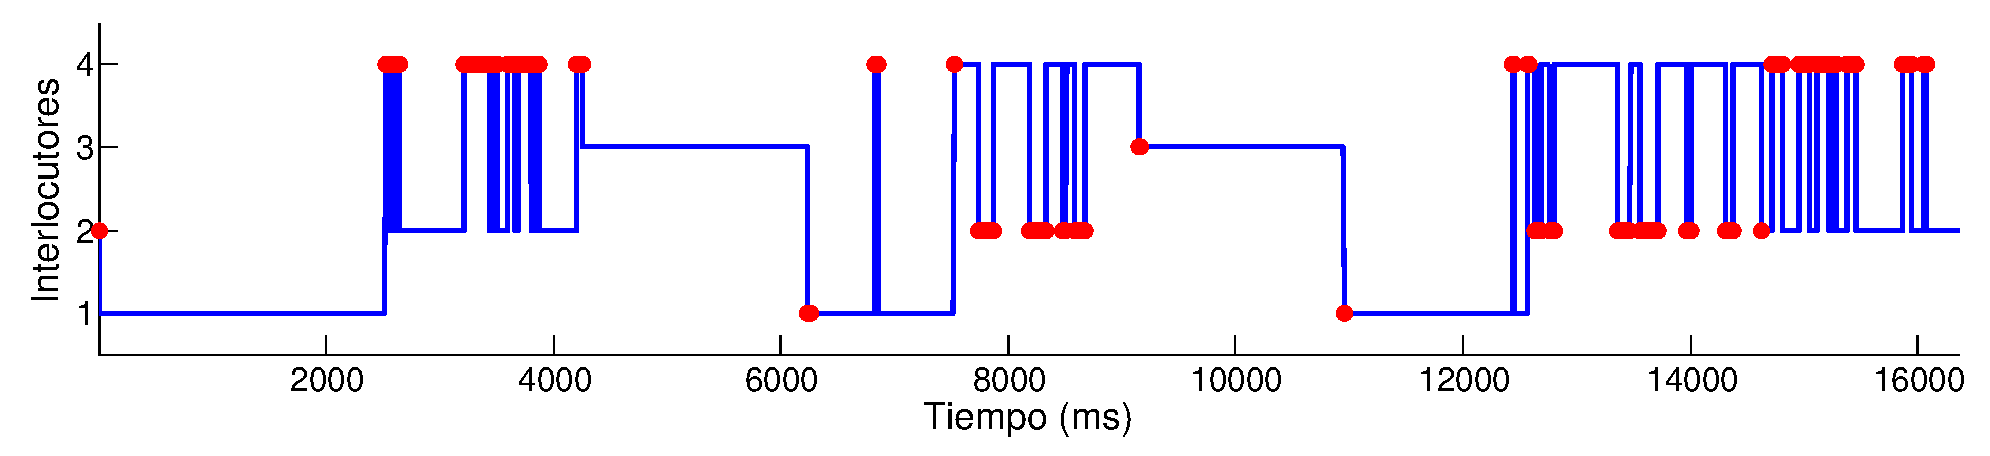
\includegraphics[width=1\linewidth]{gfx/chap6/lear3s_3_2}
      \caption{}
      \label{fig:seq3_seq2}
    \end{subfigure}
  }
  \caption[Secuencia 3: Secuencia recuperada]{En \autoref{fig:seq3_seq1} se muestra la secuencia original de la \autoref{ssub:lear}. En comparación, en \autoref{fig:seq3_seq2} se muestra la secuencia recuperada del modelo ganador y se marcan en rojo los errores cometidos respecto a la primera secuencia. }
  \label{fig:prb3_seq}
\end{figure}

Más a detalle, en la \autoref{fig:prb3_seq} se observa en azul el orden en el que participan los interlocutores de acuerdo a la secuencia recuperada. En rojo se marcan tanto los falsos positivos como los falsos negativos, de acuerdo al ground truth. Hay que notar que cuando el número de estados para un modelo no es el correcto, entonces inminentemente el número de errores en la secuencia obtenida será mayor, pues al menos todas las intervenciones de un hablante no podrán ser emparejadas o serán asignadas a alguien más.

Se observa también que la mayoría de las veces, en la secuencia recuperada se encuentran algunos brincos entre personas, pero en esencia la estructura y el orden en que hablan los interlocutores es el correcto.
 

%%%%%%%%%%%%%%%%%%%%%%%%%%%%%%%%%%%%%%%%%%%%%%%%%%%%%%%%%%%%%%% 

\subsection[Secuencia 4]{Secuencia 4: Manuel Acuña}
\label{ssub:nocturno}

  Para la cuarta secuencia se utilizaron algunos poemas del escritor Manuel Acuña, alternando 6 voces diferentes en español. La secuencia de audio original tiene una duración de 10:41 min.

Para la etapa de agrupación de los vectores MFCC con k-means++ se usaron 140 centros iniciales, mientras que el banco de filtros fue el mismo que en la secuencia anterior.

\begin{figure}[tp]
  \centerline{  
    \hspace{1.2cm}
    \parbox[c]{0.38\textwidth}{\centering Modelo generador}
    \parbox[c]{0.38\textwidth}{\centering Modelo $n_2$}
    \parbox[c]{0.38\textwidth}{\centering Modelo $n_3$}
    \parbox[c]{0.38\textwidth}{\centering Modelo $n_4$}
  }
  \vspace{0.5cm}
  \foreach \row in {1, ..., 2}{%  
    \centerline{%
      \parbox[c]{1cm}{
        \vspace{-0.5cm}
        \myheader{\row}
      }
      %\gdef \widthimg {0.35}
      \foreach \col in {1, ..., 4}{%
        \pgfmathparse{\col == 4 && \row == 2? 1:0}
        \ifthenelse{\pgfmathresult=1}{
          \gdef \widthimg {0.39}
        }{
          \gdef \widthimg {0.35}
        }
        \begin{subfigure}[c]{\widthimg \textwidth}          
          \def \imgfile {gfx/chap6/noct1p_\col_\row}
          \IfFileExists{\imgfile.eps}{
            \includegraphics[width=1\textwidth]{\imgfile}
            \label{fig:seq4p_\col_\row}
          }{
            \hspace{1\textwidth}
          }
        \end{subfigure}
        %\hspace{-0.005\textwidth}
      }
    }
  }
\caption[Secuencia 4: Parámetros estimados (1)]{Por columnas, se muestran los parámetros obtenidos para varios modelos propuestos. La primer columna corresponde a los parámetros verdaderos.
En la primer fila \textup{(a)} se muestran las probabilidades a priori de que cada uno de los interlocutores empiecen la conversación. En la segunda fila \textup{(b)} se muestra en falso color la matriz de transición entre interlocutores para cada uno de los modelos mostrados.}
\label{fig:seq4p}
\end{figure}

En las \autoref{fig:seq4p} y \autoref{fig:seq4q} se muestran los parámetros estimados para los diferentes modelos que se propusieron. La primer columna corresponde a los parámetros verdaderos, mientras que las demás columnas son los parámetros obtenidos para diferentes modelos estimados. 

En la primer fila de la \autoref{fig:seq4p} se muestran las probabilidades a priori de que cada uno de los interlocutores empiecen el diálogo. En la segunda fila se muestra en falso color la matriz de transición para cada uno de los modelos. Esta matriz representa la probabilidad de cambio entre las personas que participan en la conversación.

Se observa como en general para todos los modelos propuestos la matriz de transición que se recupera tiene una estructura diagonal, puesto que en este tipo de problemas, una persona suele hablar durante un periodo considerablemente largo, para que luego otra persona empiece a hablar.

\begin{figure}[t!]
  \centerline{
    \hspace{1.2cm}
    \parbox[c]{0.35\textwidth}{\centering Modelo generador}
    \parbox[c]{0.35\textwidth}{\centering Modelo $n_2$}
    \parbox[c]{0.35\textwidth}{\centering Modelo $n_3$}
    \parbox[c]{0.35\textwidth}{\centering Modelo $n_4$}
  }
  \vspace{0.5cm}
  \foreach \row in {3, ..., 6}{%  
    \centerline{
      \parbox[c]{1cm}{
        \vspace{-0.3cm}
        \myheader{\row}
      }
      \foreach \col in {1, ..., 4}{%
        \begin{subfigure}[c]{0.35\textwidth}  
          \def \imgfile {gfx/chap6/noct1p_\col_\row}
          \IfFileExists{\imgfile.eps}{
            \includegraphics[width=1\textwidth]{\imgfile}
            %\caption{}
            \label{fig:seq4p_\col_\row}
          }{
            \hspace{1\textwidth}
          }
        \end{subfigure}
      }
    }
  }
\caption[Secuencia 4: Parámetros estimados (2)]{Por columnas, se muestran las probabilidades de emisión para cada uno de los interlocutores de acuerdo al modelo. Cada fila representa las probabilidad de emisión de las palabras en el diccionario. La fila \textup{(c)} para la primer persona, la fila \textup{(d)} para la segunda persona y así de forma consecutiva, de acuerdo al número de personas que contempla cada modelo propuesto.}
\label{fig:seq4q}
\end{figure}

En la \autoref{fig:seq4q} se muestran las probabilidades de emisión para cada uno de los participantes, de acuerdo a las palabras en las que se ha discretizado la conversación. Idealmente, cada interlocutor tiene asignadas con mayor probabilidad un cierto conjunto de palabras del diccionario, lo que hace que la identificación de las personas sea mucho más fácil de realizar.

Para la selección del modelo y siguiendo la metodología propuesta, primero se efectúa una inspección por medio de BIC regularizado para encontrar cuál o cuáles son los modelos más probables.

\begin{figure}[t!]
  \centerline{
  \begin{subfigure}[b]{1.1\textwidth}
   \includegraphics[width=1\textwidth]{gfx/chap6/noct1bic2}
   \caption{}
   \label{fig:seq4_bic2}
  \end{subfigure}  
  }  
  \centerline{
  \begin{subfigure}[b]{0.55\textwidth}
    \includegraphics[width=\textwidth]{gfx/chap6/noct1bic1} 
    \caption{}
    \label{fig:seq4_bic1}
  \end{subfigure}  
  \begin{subfigure}[b]{0.55\textwidth}
    \includegraphics[width=\textwidth]{gfx/chap6/lear3bic3} 
    \caption{}
    \label{fig:seq4_bic3}
  \end{subfigure}
  }
  \caption[Secuencia 4: Pruebas BIC]{En la \autoref{fig:seq4_bic2}, se muestra las curvas de nivel de la superficie al variar el valor de lambda para evaluar BIC, así como la dirección del gradiente en la misma. En la \autoref{fig:seq4_bic1} se muestra una perspectiva general de superficie en \autoref{fig:seq4_bic2}. En la \autoref{fig:seq4_bic3} se muestra el valor seleccionado para lambda de acuerdo al análisis de sensibilidad realizado en la superficie anterior.}
  \label{fig:seq4_bic}
\end{figure}

En la \autoref{fig:seq4_bic1} se muestra la superficie generada al variar el valor de $\lambda$ para diferentes curvas de selección BIC. Se observa cómo al principio $\lambda$ es muy pequeño, y entonces el término de penalización no funciona por lo que se prefieren los modelos más complejos y sobre ajustados. Por otro lado, cuando $\lambda$ es muy grande, la penalización no permite mas que escoger los modelos más simples.

Haciendo un análisis de sensibilidad se puede determinar cuál es el parámetro $\lambda$ adecuado que penaliza de buena forma la log-verosimilitud.

En la \autoref{fig:seq4_bic2} se muestran las curvas de nivel de la figura anterior, además de la dirección del gradiente de la misma. Así mismo, en falso color se resaltan las zonas en las que el gradiente es menor. 

Lo que nos interesa encontrar en la superficie, es el valor de $\lambda$ que representa el punto de inflexión entre la selección de modelos demasiado complejos y modelos más simples. Para esto, se busca la zona en la que el gradiente sea lo más cercano a cero, pues implicaría que es un punto crítico.

Debido a la escala y a la forma en la que se calculó el gradiente, aunque para algunos valores cercanos de $\lambda$ no haya mucha variación en esa dirección; si BIC está penalizando mal, entonces sí habrá gran variación para los diferentes modelos. Es por esto, que sólo en la zona en que la penalización sea del mismo orden de magnitud que la verosimilitud la variación en la curva BIC con el $\lambda$ adecuado no será tan grande como en otras zonas.

Por último, se muestra en \autoref{fig:seq4_bic3} la curva BIC con el valor de $\lambda$ encontrado a partir del análisis de sensibilidad realizado en la \autoref{fig:seq4_bic2}. El o los modelos que tengan un mayor valor BIC serán los que se seleccionarán como modelos ganadores.

\begin{figure}[t!]
  \centerline  
  { \begin{subfigure}[b]{0.7\textwidth}
      \includegraphics[width=1\linewidth]{gfx/chap6/noct1boot1}
      \caption{}
      \label{fig:seq4_boot1}
    \end{subfigure}
    \hspace{0.5cm}
    \begin{subfigure}[b]{0.7\textwidth}
      \includegraphics[width=1\linewidth]{gfx/chap6/noct1boot2}
      \caption{}
      \label{fig:seq4_boot2}
    \end{subfigure}
  }
  \centerline  
  { \begin{subfigure}[b]{0.7\textwidth}
      \includegraphics[width=1\linewidth]{gfx/chap6/noct1boot3}
      \caption{}
      \label{fig:seq4_boot3}
    \end{subfigure}
    \hspace{0.5cm}
    \begin{subfigure}[b]{0.7\textwidth}
      \includegraphics[width=1\linewidth]{gfx/chap6/noct1boot4}
      \caption{}
      \label{fig:seq4_boot4}
    \end{subfigure}
  }
  \caption[Secuencia 4: Pruebas de hipótesis usando bootstrap]{En la \autoref{fig:seq4_boot1} se muestra la prueba de hipótesis realizada para comparar el modelo $n_4$ contra $n_5$. Como se observa, se rechaza la hipótesis de que el modelo correcto sea $n_4$. En la \autoref{fig:seq4_boot2} se hace la prueba del modelo $n_5$ contra $n_6$, y de la misma manera, se rechaza la hipótesis de que el modelo correcto sea $n_5$. Se sigue con la prueba de hipótesis del modelo $n_6$ contra $n_7$ en la \autoref{fig:seq4_boot3}, y en este caso el valor observado no cae dentro de la región de rechazo, por lo que no podemos rechazar que el modelo $n_6$ sea el correcto. Por último en la \autoref{fig:seq4_boot4}, se hace la prueba del modelo $n_7$ contra el modelo $n_8$, y se vuelve a rechazar la hipótesis nula.}  
  \label{fig:seq4_boot}
\end{figure}

En caso de que después de utilizar BIC se presente ambigüedad para determinar un modelo ganador, o ya sea para realizar un análisis más exhaustivo, se puede propone hacer una prueba de hipótesis para determinar cuál modelo se ajusta mejor a los datos.

A diferencia de la primer etapa, en la que se usa BIC como criterio para  seleccionar el mejor modelo de un conjunto no definido de modelos con diferentes parámetros, la intención de hacer pruebas de hipótesis es determinar en un pequeño conjunto de probables modelos, cuál es mejor, y qué tan bueno es un modelo respecto a otro.

Al plantear la prueba de hipótesis se harán una gran cantidad de simulaciones para ver qué tan bien se ajusta cada modelo a los datos originales, por lo que este proceso es computacionalmente intensivo y sólo se recomienda hacerlo para evitar la ambigüedad entre un par de modelos.

...

Por último, ya con el modelo seleccionado, se procede a calcular el error relativo de predicción que se obtuvo, comparando con el ground truth que se dispone para esa secuencia, con lo que se obtiene: 

...

\begin{figure}[tp]
  \centerline
  {\begin{subfigure}[b]{1.3\textwidth}
      \includegraphics[width=1\linewidth]{gfx/chap6/noct1s_3_1}
      \caption{}
      \label{fig:seq4_seq1}
    \end{subfigure}
  } 
  \centerline
  {\begin{subfigure}[b]{1.3\textwidth}
      \includegraphics[width=1\linewidth]{gfx/chap6/noct1s_3_2}
      \caption{}
      \label{fig:seq4_seq2}
    \end{subfigure}
  }
  \caption[Secuencia 4: Secuencia recuperada]{En \autoref{fig:seq4_seq1} se muestra la secuencia original de la \autoref{ssub:nocturno}. En comparación, en \autoref{fig:seq4_seq2} se muestra la secuencia recuperada del modelo ganador y se marcan en rojo los errores cometidos respecto a la primera secuencia. }
  \label{fig:prb4_seq}
\end{figure}

Más a detalle, en la \autoref{fig:prb4_seq} se observa en azul el orden en el que participan los interlocutores de acuerdo a la secuencia recuperada. En rojo se marcan tanto los falsos positivos como los falsos negativos, de acuerdo al ground truth. Hay que notar que cuando el número de estados para un modelo no es el correcto, entonces inminentemente el número de errores en la secuencia obtenida será mayor, pues al menos todas las intervenciones de un hablante no podrán ser emparejadas o serán asignadas a alguien más.

Se observa también que la mayoría de las veces, en la secuencia recuperada se encuentran algunos brincos entre personas, pero en esencia la estructura y el orden en que hablan los interlocutores es el correcto.
 

%%%%%%%%%%%%%%%%%%%%%%%%%%%%%%%%%%%%%%%%%%%%%%%%%%%%%%%%%%%%%%% 

\subsection[Secuencia 5]{Secuencia 5: Calderón de la Barca}
\label{ssub:calderon}

  En esta quinta secuencia se trabajó con varios fragmentos del poema 'La vida es sueño' del escritor Pedro Calderón de la Barca, usándose 3 diferentes voces en español. La secuencia de audio original es de 11:18 min.

Para la etapa de agrupación de los vectores MFCC con k-means++ se usaron 160 centros iniciales, mientras que el banco de filtros fue el usado en las secuencias anteriores.

\begin{figure}[bht]
  \centerline{  
    \hspace{1.2cm}
    \parbox[c]{0.38\textwidth}{\centering Modelo generador}
    \parbox[c]{0.38\textwidth}{\centering Modelo $n_2$}
    \parbox[c]{0.38\textwidth}{\centering Modelo $n_3$}
    \parbox[c]{0.38\textwidth}{\centering Modelo $n_4$}
  }
  \vspace{0.5cm}
  \foreach \row in {1, ..., 2}{%  
    \centerline{%
      \parbox[c]{1cm}{
        \vspace{-0.5cm}
        \myheader{\row}
      }
      %\gdef \widthimg {0.35}
      \foreach \col in {1, ..., 4}{%
        \pgfmathparse{\col == 4 && \row == 2? 1:0}
        \ifthenelse{\pgfmathresult=1}{
          \gdef \widthimg {0.39}
        }{
          \gdef \widthimg {0.35}
        }
        \begin{subfigure}[c]{\widthimg \textwidth}          
          \def \imgfile {gfx/chap6/calderon1p_\col_\row}
          \IfFileExists{\imgfile.eps}{
            \includegraphics[width=1\textwidth]{\imgfile}
            \label{fig:seq5p_\col_\row}
          }{
            \hspace{1\textwidth}
          }
        \end{subfigure}
        %\hspace{-0.005\textwidth}
      }
    }
  }
\caption[Secuencia 5: Parámetros estimados (1)]{Por columnas, se muestran los parámetros obtenidos para varios modelos propuestos. La primer columna corresponde a los parámetros verdaderos.
En la primer fila \textup{(a)} se muestran las probabilidades a priori de que cada uno de los interlocutores empiecen la conversación. En la segunda fila \textup{(b)} se muestra en falso color la matriz de transición entre interlocutores para cada uno de los modelos mostrados.}
\label{fig:seq5p}
\end{figure}

En las \autoref{fig:seq5p} y \autoref{fig:seq5q} se muestran los parámetros estimados para los diferentes modelos que se propusieron. La primer columna corresponde a los parámetros verdaderos, mientras que las demás columnas son los parámetros obtenidos para diferentes modelos estimados. 

En la primer fila de la \autoref{fig:seq5p} se muestran las probabilidades a priori de que cada uno de los interlocutores empiecen el diálogo. En la segunda fila se muestra en falso color la matriz de transición para cada uno de los modelos. Esta matriz representa la probabilidad de cambio entre las personas que participan en la conversación.

Se observa como en general para todos los modelos propuestos la matriz de transición que se recupera tiene una estructura diagonal, puesto que en este tipo de problemas, una persona suele hablar durante un periodo considerablemente largo, para que luego otra persona empiece a hablar.

\begin{figure}[t!]
  \centerline{
    \hspace{1.2cm}
    \parbox[c]{0.35\textwidth}{\centering Modelo generador}
    \parbox[c]{0.35\textwidth}{\centering Modelo $n_2$}
    \parbox[c]{0.35\textwidth}{\centering Modelo $n_3$}
    \parbox[c]{0.35\textwidth}{\centering Modelo $n_4$}
  }
  \vspace{0.5cm}
  \foreach \row in {3, ..., 6}{%  
    \centerline{
      \parbox[c]{1cm}{
        \vspace{-0.3cm}
        \myheader{\row}
      }
      \foreach \col in {1, ..., 4}{%
        \begin{subfigure}[c]{0.35\textwidth}  
          \def \imgfile {gfx/chap6/calderon1p_\col_\row}
          \IfFileExists{\imgfile.eps}{
            \includegraphics[width=1\textwidth]{\imgfile}
            %\caption{}
            \label{fig:seq5p_\col_\row}
          }{
            \hspace{1\textwidth}
          }
        \end{subfigure}
      }
    }
  }
\caption[Secuencia 5: Parámetros estimados (2)]{Por columnas, se muestran las probabilidades de emisión para cada uno de los interlocutores de acuerdo al modelo. Cada fila representa las probabilidad de emisión de las palabras en el diccionario. La fila \textup{(c)} para la primer persona, la fila \textup{(d)} para la segunda persona y así de forma consecutiva, de acuerdo al número de personas que contempla cada modelo propuesto.}
\label{fig:seq5q}
\end{figure}

En la \autoref{fig:seq5q} se muestran las probabilidades de emisión para cada uno de los participantes, de acuerdo a las palabras en las que se ha discretizado la conversación. Idealmente, cada interlocutor tiene asignadas con mayor probabilidad un cierto conjunto de palabras del diccionario, lo que hace que la identificación de las personas sea mucho más fácil de realizar.

Para la selección del modelo y siguiendo la metodología propuesta, primero se efectúa una inspección por medio de BIC regularizado para encontrar cuál o cuáles son los modelos más probables.

\begin{figure}[t!]
  \centerline{
  \begin{subfigure}[b]{1.1\textwidth}
   \includegraphics[width=1\textwidth]{gfx/chap6/calderon1bic2}
   \caption{}
   \label{fig:seq5_bic2}
  \end{subfigure}  
  }  
  \centerline{
  \begin{subfigure}[b]{0.55\textwidth}
    \includegraphics[width=\textwidth]{gfx/chap6/calderon1bic1} 
    \caption{}
    \label{fig:seq5_bic1}
  \end{subfigure}  
  \begin{subfigure}[b]{0.55\textwidth}
    \includegraphics[width=\textwidth]{gfx/chap6/calderon1bic3} 
    \caption{}
    \label{fig:seq5_bic3}
  \end{subfigure}
  }
  \caption[Secuencia 5: Pruebas BIC]{En la \autoref{fig:seq5_bic2}, se muestra las curvas de nivel de la superficie al variar el valor de lambda para evaluar BIC, así como la dirección del gradiente en la misma. En la \autoref{fig:seq5_bic1} se muestra una perspectiva general de superficie en \autoref{fig:seq5_bic2}. En la \autoref{fig:seq5_bic3} se muestra el valor seleccionado para lambda de acuerdo al análisis de sensibilidad realizado en la superficie anterior.}
  \label{fig:seq1_bic}
\end{figure}

En la \autoref{fig:seq5_bic1} se muestra la superficie generada al variar el valor de $\lambda$ para diferentes curvas de selección BIC. Se observa cómo al principio $\lambda$ es muy pequeño, y entonces el término de penalización no funciona por lo que se prefieren los modelos más complejos y sobre ajustados. Por otro lado, cuando $\lambda$ es muy grande, la penalización no permite mas que escoger los modelos más simples.

Haciendo un análisis de sensibilidad se puede determinar cuál es el parámetro $\lambda$ adecuado que penaliza de buena forma la log-verosimilitud.

En la \autoref{fig:seq5_bic2} se muestran las curvas de nivel de la figura anterior, además de la dirección del gradiente de la misma. Así mismo, en falso color se resaltan las zonas en las que el gradiente es menor. 

Lo que nos interesa encontrar en la superficie, es el valor de $\lambda$ que representa el punto de inflexión entre la selección de modelos demasiado complejos y modelos más simples. Para esto, se busca la zona en la que el gradiente sea lo más cercano a cero, pues implicaría que es un punto crítico.

Debido a la escala y a la forma en la que se calculó el gradiente, aunque para algunos valores cercanos de $\lambda$ no haya mucha variación en esa dirección; si BIC está penalizando mal, entonces sí habrá gran variación para los diferentes modelos. Es por esto, que sólo en la zona en que la penalización sea del mismo orden de magnitud que la verosimilitud la variación en la curva BIC con el $\lambda$ adecuado no será tan grande como en otras zonas.

Por último, se muestra en \autoref{fig:seq5_bic3} la curva BIC con el valor de $\lambda$ encontrado a partir del análisis de sensibilidad realizado en la \autoref{fig:seq5_bic2}. El o los modelos que tengan un mayor valor BIC serán los que se seleccionarán como modelos ganadores.

\begin{figure}[t!]
  \centerline  
  { \begin{subfigure}[b]{0.7\textwidth}
      \includegraphics[width=1\linewidth]{gfx/chap6/calderon1boot1}
      \caption{}
      \label{fig:seq5_boot1}
    \end{subfigure}
    \hspace{0.5cm}
    \begin{subfigure}[b]{0.7\textwidth}
      \includegraphics[width=1\linewidth]{gfx/chap6/calderon1boot2}
      \caption{}
      \label{fig:seq5_boot2}
    \end{subfigure}
  }
  \centerline  
  { \begin{subfigure}[b]{0.7\textwidth}
      \includegraphics[width=1\linewidth]{gfx/chap6/calderon1boot3}
      \caption{}
      \label{fig:seq5_boot3}
    \end{subfigure}
    \hspace{0.5cm}
    \begin{subfigure}[b]{0.7\textwidth}
      \includegraphics[width=1\linewidth]{gfx/chap6/calderon1boot4}
      \caption{}
      \label{fig:seq5_boot4}
    \end{subfigure}
  }
  \caption[Secuencia 5: Pruebas de hipótesis usando bootstrap]{En la \autoref{fig:seq5_boot1} se muestra la prueba de hipótesis realizada para comparar el modelo $n_2$ contra $n_3$. Como se observa, se rechaza la hipótesis de que el modelo correcto sea $n_2$. En la \autoref{fig:seq5_boot2} se hace la prueba del modelo $n_3$ contra $n_4$, y se vuelve a rechazar la hipótesis nula, aunque queda muy cerca del umbral de decisión. Realizando la prueba de $n_4$ contra $n_5$ en la \autoref{fig:seq5_boot3} en este caso el valor observado no cae dentro de la región de rechazo, por lo que no podemos rechazar que el modelo $n_4$ sea el correcto. Por último en la \autoref{fig:seq5_boot4}, se hace la prueba del modelo $n_5$ contra el modelo $n_5$, y vuelve a suceder lo mismo que en el caso anterior. Como para las últimas dos pruebas no se pudo rechazar la hipótesis nula, se preferirá siempre la que involucre al modelo más sencillo. Cabe recalcar también que si se hicieran las pruebas de hipótesis con una significancia menor, entonces desde la segunda prueba se tendría al modelo ganador,}
  \label{fig:seq5_boot}
\end{figure}

En caso de que después de utilizar BIC se presente ambigüedad para determinar un modelo ganador, o ya sea para realizar un análisis más exhaustivo, se puede propone hacer una prueba de hipótesis para determinar cuál modelo se ajusta mejor a los datos.

A diferencia de la primer etapa, en la que se usa BIC como criterio para  seleccionar el mejor modelo de un conjunto no definido de modelos con diferentes parámetros, la intención de hacer pruebas de hipótesis es determinar en un pequeño conjunto de probables modelos, cuál es mejor, y qué tan bueno es un modelo respecto a otro.

Al plantear la prueba de hipótesis se harán una gran cantidad de simulaciones para ver qué tan bien se ajusta cada modelo a los datos originales, por lo que este proceso es computacionalmente intensivo y sólo se recomienda hacerlo para evitar la ambigüedad entre un par de modelos.

...

Por último, ya con el modelo seleccionado, se procede a calcular el error relativo de predicción que se obtuvo, comparando con el ground truth que se dispone para esa secuencia, con lo que se obtiene: 

...

\begin{figure}[bht]
  \centerline
  {\begin{subfigure}[b]{1.3\textwidth}
      \includegraphics[width=1\linewidth]{gfx/chap6/calderon1s_3_1}
      \caption{}
      \label{fig:seq5_seq1}
    \end{subfigure}
  } 
  \centerline
  {\begin{subfigure}[b]{1.3\textwidth}
      \includegraphics[width=1\linewidth]{gfx/chap6/calderon1s_4_2}
      \caption{}
      \label{fig:seq5_seq3}
    \end{subfigure}
  }    
  \centerline
  {\begin{subfigure}[b]{1.3\textwidth}
      \includegraphics[width=1\linewidth]{gfx/chap6/calderon1s_3_2}
      \caption{}
      \label{fig:seq5_seq2}
    \end{subfigure}
  }
  \caption[Secuencia 5: Secuencia recuperada]{En \autoref{fig:seq5_seq1} se muestra la secuencia original de la \autoref{ssub:calderon}. En comparación, en \autoref{fig:seq5_seq3} se muestra la secuencia recuperada del modelo ganador y se marcan en rojo los errores cometidos respecto a la primera secuencia. Por último, se muestra en \autoref{fig:seq5_seq2} la el modelo que debió haber ganado en caso de que se usara una significacia más baja para las pruebas.}
  \label{fig:prb5_seq}
\end{figure}

Más a detalle, en la \autoref{fig:prb5_seq} se observa en azul el orden en el que participan los interlocutores de acuerdo a la secuencia recuperada. En rojo se marcan tanto los falsos positivos como los falsos negativos, de acuerdo al ground truth. Hay que notar que cuando el número de estados para un modelo no es el correcto, entonces inminentemente el número de errores en la secuencia obtenida será mayor, pues al menos todas las intervenciones de un hablante no podrán ser emparejadas o serán asignadas a alguien más.

Se observa también que la mayoría de las veces, en la secuencia recuperada se encuentran algunos brincos entre personas, pero en esencia la estructura y el orden en que hablan los interlocutores es el correcto.
 
  
%%%%%%%%%%%%%%%%%%%%%%%%%%%%%%%%%%%%%%%%%%%%%%%%%%%%%%%%%%%%%%% 

\subsection[Secuencia 6]{Secuencia 6: Andrew Lloyd Webber}
\label{ssub:cats}

  Para la última secuencia de prueba se utilizaron fragmentos de la obra musical 'Cats', escrita por Andrew Lloyd Webber, usando 5 voces distintas en inglés. La secuencia de audio original tiene una duración de 6:48 min.

Para la etapa de agrupación de los vectores MFCC con k-means++ se usaron 90 centros iniciales, usando el mismo banco de filtros.

\begin{figure}[tp]
  \centerline{  
    \hspace{1.2cm}
    \parbox[c]{0.38\textwidth}{\centering Modelo generador}
    \parbox[c]{0.38\textwidth}{\centering Modelo $n_4$}
    \parbox[c]{0.38\textwidth}{\centering Modelo $n_5$}
    \parbox[c]{0.38\textwidth}{\centering Modelo $n_6$}
  }
  \vspace{0.5cm}
  \foreach \row in {1, ..., 2}{%  
    \centerline{%
      \parbox[c]{1cm}{
        \vspace{-0.5cm}
        \myheader{\row}
      }
      %\gdef \widthimg {0.35}
      \foreach \col in {1, ..., 4}{%
        \pgfmathparse{\col == 4 && \row == 2? 1:0}
        \ifthenelse{\pgfmathresult=1}{
          \gdef \widthimg {0.39}
        }{
          \gdef \widthimg {0.35}
        }
        \begin{subfigure}[c]{\widthimg \textwidth}          
          \def \imgfile {gfx/chap6/cats1p_\col_\row}
          \IfFileExists{\imgfile.eps}{
            \includegraphics[width=1\textwidth]{\imgfile}
            \label{fig:seq6p_\col_\row}
          }{
            \hspace{1\textwidth}
          }
        \end{subfigure}
        %\hspace{-0.005\textwidth}
      }
    }
  }
\caption[Secuencia 6: Parámetros estimados (1)]{Por columnas, se muestran los parámetros obtenidos para varios modelos propuestos. La primer columna corresponde a los parámetros verdaderos.
En la primer fila \textup{(a)} se muestran las probabilidades a priori de que cada uno de los interlocutores empiecen la conversación. En la segunda fila \textup{(b)} se muestra en falso color la matriz de transición entre interlocutores para cada uno de los modelos mostrados.}
\label{fig:seq6p}
\end{figure}

En las \autoref{fig:seq6p} y \autoref{fig:seq6q} se muestran los parámetros estimados para los diferentes modelos que se propusieron. La primer columna corresponde a los parámetros verdaderos, mientras que las demás columnas son los parámetros obtenidos para diferentes modelos estimados. 

En la primer fila de la \autoref{fig:seq6p} se muestran las probabilidades a priori de que cada uno de los interlocutores empiecen el diálogo. En la segunda fila se muestra en falso color la matriz de transición para cada uno de los modelos. Esta matriz representa la probabilidad de cambio entre las personas que participan en la conversación.

Se observa como en general para todos los modelos propuestos la matriz de transición que se recupera tiene una estructura diagonal, puesto que en este tipo de problemas, una persona suele hablar durante un periodo considerablemente largo, para que luego otra persona empiece a hablar.

\begin{figure}[t!]
  \centerline{
    \hspace{1.2cm}
    \parbox[c]{0.35\textwidth}{\centering Modelo generador}
    \parbox[c]{0.35\textwidth}{\centering Modelo $n_4$}
    \parbox[c]{0.35\textwidth}{\centering Modelo $n_5$}
    \parbox[c]{0.35\textwidth}{\centering Modelo $n_6$}
  }
  \vspace{0.5cm}
  \foreach \row in {3, ..., 8}{%  
    \centerline{
      \parbox[c]{1cm}{
        \vspace{-0.3cm}
        \myheader{\row}
      }
      \foreach \col in {1, ..., 4}{%
        \begin{subfigure}[c]{0.35\textwidth}  
          \def \imgfile {gfx/chap6/cats1p_\col_\row}
          \IfFileExists{\imgfile.eps}{
            \includegraphics[width=1\textwidth]{\imgfile}
            %\caption{}
            \label{fig:seq6p_\col_\row}
          }{
            \hspace{1\textwidth}
          }
        \end{subfigure}
      }
    }
  }
\caption[Secuencia 6: Parámetros estimados (2)]{Por columnas, se muestran las probabilidades de emisión para cada uno de los interlocutores de acuerdo al modelo. Cada fila representa las probabilidad de emisión de las palabras en el diccionario. La fila \textup{(c)} para la primer persona, la fila \textup{(d)} para la segunda persona y así de forma consecutiva, de acuerdo al número de personas que contempla cada modelo propuesto.}
\label{fig:seq6q}
\end{figure}

En la \autoref{fig:seq6q} se muestran las probabilidades de emisión para cada uno de los participantes, de acuerdo a las palabras en las que se ha discretizado la conversación. Idealmente, cada interlocutor tiene asignadas con mayor probabilidad un cierto conjunto de palabras del diccionario, lo que hace que la identificación de las personas sea mucho más fácil de realizar.

Para la selección del modelo y siguiendo la metodología propuesta, primero se efectúa una inspección por medio de BIC regularizado para encontrar cuál o cuáles son los modelos más probables.

\begin{figure}[t!]
  \centerline{
  \begin{subfigure}[b]{1.1\textwidth}
   \includegraphics[width=1\textwidth]{gfx/chap6/noct1bic2}
   \caption{}
   \label{fig:seq6_bic2}
  \end{subfigure}  
  }  
  \centerline{
  \begin{subfigure}[b]{0.55\textwidth}
    \includegraphics[width=\textwidth]{gfx/chap6/noct1bic1} 
    \caption{}
    \label{fig:seq6_bic1}
  \end{subfigure}  
  \begin{subfigure}[b]{0.55\textwidth}
    \includegraphics[width=\textwidth]{gfx/chap6/lear3bic3} 
    \caption{}
    \label{fig:seq6_bic3}
  \end{subfigure}
  }
  \caption[Secuencia 6: Pruebas BIC]{En la \autoref{fig:seq6_bic2}, se muestra las curvas de nivel de la superficie al variar el valor de lambda para evaluar BIC, así como la dirección del gradiente en la misma. En la \autoref{fig:seq6_bic1} se muestra una perspectiva general de superficie en \autoref{fig:seq6_bic2}. En la \autoref{fig:seq6_bic3} se muestra el valor seleccionado para lambda de acuerdo al análisis de sensibilidad realizado en la superficie anterior.}
  \label{fig:seq6_bic}
\end{figure}

En la \autoref{fig:seq6_bic1} se muestra la superficie generada al variar el valor de $\lambda$ para diferentes curvas de selección BIC. Se observa cómo al principio $\lambda$ es muy pequeño, y entonces el término de penalización no funciona por lo que se prefieren los modelos más complejos y sobre ajustados. Por otro lado, cuando $\lambda$ es muy grande, la penalización no permite mas que escoger los modelos más simples.

Haciendo un análisis de sensibilidad se puede determinar cuál es el parámetro $\lambda$ adecuado que penaliza de buena forma la log-verosimilitud.

En la \autoref{fig:seq6_bic2} se muestran las curvas de nivel de la figura anterior, además de la dirección del gradiente de la misma. Así mismo, en falso color se resaltan las zonas en las que el gradiente es menor. 

Lo que nos interesa encontrar en la superficie, es el valor de $\lambda$ que representa el punto de inflexión entre la selección de modelos demasiado complejos y modelos más simples. Para esto, se busca la zona en la que el gradiente sea lo más cercano a cero, pues implicaría que es un punto crítico.

Debido a la escala y a la forma en la que se calculó el gradiente, aunque para algunos valores cercanos de $\lambda$ no haya mucha variación en esa dirección; si BIC está penalizando mal, entonces sí habrá gran variación para los diferentes modelos. Es por esto, que sólo en la zona en que la penalización sea del mismo orden de magnitud que la verosimilitud la variación en la curva BIC con el $\lambda$ adecuado no será tan grande como en otras zonas.

Por último, se muestra en \autoref{fig:seq6_bic3} la curva BIC con el valor de $\lambda$ encontrado a partir del análisis de sensibilidad realizado en la \autoref{fig:seq6_bic2}. El o los modelos que tengan un mayor valor BIC serán los que se seleccionarán como modelos ganadores.

\begin{figure}[t!]
  \centerline  
  { \begin{subfigure}[b]{0.7\textwidth}
      \includegraphics[width=1\linewidth]{gfx/chap6/cats1boot1}
      \caption{}
      \label{fig:seq6_boot1}
    \end{subfigure}
    \hspace{0.5cm}
    \begin{subfigure}[b]{0.7\textwidth}
      \includegraphics[width=1\linewidth]{gfx/chap6/cats1boot2}
      \caption{}
      \label{fig:seq6_boot2}
    \end{subfigure}
  }
  \centerline  
  { \begin{subfigure}[b]{0.7\textwidth}
      \includegraphics[width=1\linewidth]{gfx/chap6/cats1boot3}
      \caption{}
      \label{fig:seq6_boot3}
    \end{subfigure}
    \hspace{0.5cm}
    \begin{subfigure}[b]{0.7\textwidth}
      \includegraphics[width=1\linewidth]{gfx/chap6/cats1boot4}
      \caption{}
      \label{fig:seq6_boot4}
    \end{subfigure}
  }
  \caption[Secuencia 6: Pruebas de hipótesis usando bootstrap]{En la \autoref{fig:seq6_boot1} se muestra la prueba de hipótesis realizada para comparar el modelo $n_4$ contra $n_5$. Como se observa, se rechaza la hipótesis de que el modelo correcto sea $n_4$. En la \autoref{fig:seq6_boot2} se hace la prueba del modelo $n_5$ contra $n_6$, y de la misma manera, se rechaza la hipótesis de que el modelo correcto sea $n_5$. Se sigue con la prueba de hipótesis del modelo $n_6$ contra $n_7$ en la \autoref{fig:seq6_boot3}, y en este caso el valor observado no cae dentro de la región de rechazo, por lo que no podemos rechazar que el modelo $n_6$ sea el correcto. Por último en la \autoref{fig:seq6_boot4}, se hace la prueba del modelo $n_7$ contra el modelo $n_8$, y se vuelve a rechazar la hipótesis nula.}  
  \label{fig:seq4_boot}
\end{figure}

En caso de que después de utilizar BIC se presente ambigüedad para determinar un modelo ganador, o ya sea para realizar un análisis más exhaustivo, se puede propone hacer una prueba de hipótesis para determinar cuál modelo se ajusta mejor a los datos.

A diferencia de la primer etapa, en la que se usa BIC como criterio para  seleccionar el mejor modelo de un conjunto no definido de modelos con diferentes parámetros, la intención de hacer pruebas de hipótesis es determinar en un pequeño conjunto de probables modelos, cuál es mejor, y qué tan bueno es un modelo respecto a otro.

Al plantear la prueba de hipótesis se harán una gran cantidad de simulaciones para ver qué tan bien se ajusta cada modelo a los datos originales, por lo que este proceso es computacionalmente intensivo y sólo se recomienda hacerlo para evitar la ambigüedad entre un par de modelos.

...

Por último, ya con el modelo seleccionado, se procede a calcular el error relativo de predicción que se obtuvo, comparando con el ground truth que se dispone para esa secuencia, con lo que se obtiene: 

...

\begin{figure}[tp]
  \centerline
  {\begin{subfigure}[b]{1.3\textwidth}
      \includegraphics[width=1\linewidth]{gfx/chap6/cats1s_3_1}
      \caption{}
      \label{fig:seq6_seq1}
    \end{subfigure}
  } 
  \centerline
  {\begin{subfigure}[b]{1.3\textwidth}
      \includegraphics[width=1\linewidth]{gfx/chap6/cats1s_3_2}
      \caption{}
      \label{fig:seq6_seq2}
    \end{subfigure}
  }
  \caption[Secuencia 6: Secuencia recuperada]{En \autoref{fig:seq6_seq1} se muestra la secuencia original de la \autoref{ssub:cats}. En comparación, en \autoref{fig:seq6_seq2} se muestra la secuencia recuperada del modelo ganador y se marcan en rojo los errores cometidos respecto a la primera secuencia. }
  \label{fig:prb6_seq}
\end{figure}

Más a detalle, en la \autoref{fig:prb6_seq} se observa en azul el orden en el que participan los interlocutores de acuerdo a la secuencia recuperada. En rojo se marcan tanto los falsos positivos como los falsos negativos, de acuerdo al ground truth. Hay que notar que cuando el número de estados para un modelo no es el correcto, entonces inminentemente el número de errores en la secuencia obtenida será mayor, pues al menos todas las intervenciones de un hablante no podrán ser emparejadas o serán asignadas a alguien más.

Se observa también que la mayoría de las veces, en la secuencia recuperada se encuentran algunos brincos entre personas, pero en esencia la estructura y el orden en que hablan los interlocutores es el correcto.
   


%!TEX root = ../Base.tex

\chapter{Conclusiones}\label{ch:chap6}

%\include{multiToC} % <--- just debug stuff, ignore for your documents

% ********************************************************************
% Backmatter
%*******************************************************
%\appendix
%\cleardoublepage
%\part{Apéndice}
%%********************************************************************
% Appendix
%*******************************************************
% If problems with the headers: get headings in appendix etc. right
%\markboth{\spacedlowsmallcaps{Appendix}}{\spacedlowsmallcaps{Appendix}}
\chapter{Appendix Test}
Lorem ipsum at nusquam appellantur his, ut eos erant homero
concludaturque. Albucius appellantur deterruisset id eam, vivendum
partiendo dissentiet ei ius. Vis melius facilisis ea, sea id convenire
referrentur, takimata adolescens ex duo. Ei harum argumentum per. Eam
vidit exerci appetere ad, ut vel zzril intellegam interpretaris.

\begin{comment}
Entonces, es importante recordar algunas propiedades de una cadena de Márkov, que ennumera Jordan (paper 2007) y que se pueden deducir usando el teorema de separación-d.
\begin{align}
\begin{split}
  p(\mb{X} \,|\, z_n) =~ &p(x_1, ..., x_n \,|\, z_n) 
  \\ &p(x_{n+1}, ..., x_N \,|\, z_n)
\end{split} \label{eqn:3-10} \\
p(x_1, ..., x_{n-1} \,|\, x_n, z_n) =~ 
  &p(x_1, ..., x_{n-1} \,|\, z_n) 
\label{eqn:3-11} \\
p(x_1, ..., x_{n-1} \,|\, z_{n-1}, z_n) =~ 
  &p(x_1, ..., x_{n-1} \,|\, z_{n-1}) 
\label{eqn:3-12} \\
p(x_{n+1}, ..., x_N \,|\, z_n, z_{n+1}) =~ 
  &p(x_{n+1}, ..., x_N \,|\, z_{n+1}) 
\label{eqn:3-13} \\
p(x_{n+2}, ..., x_N \,|\, z_{n+1}, x_{n+1}) =~ 
  &p(x_{n+2}, ..., x_N \,|\, z_{n+1}11 
\label{eqn:3-14} \\ 
\begin{split}
  p(\mb{X} \,|\, z_{n-1}, z_n) =~ &p(x_1, ..., x_{n-1} \,|\, z_{n-1}) 
  \\ &p(x_n \,|\, z_n) 
  \\ &p(x_{n+1}, ..., x_N | z_n)
\end{split} \label{eqn:3-15} \\
  p(x_{N+1} \,|\, \mb{X} ,z_{N+1}) =~ &p(x_{N+1} \,|\, z_{N+1}) 
\label{eqn:3-16} \\
p(z_{N+1} \,|\, z_N, \mb{X}) =~ &p(z_{N+1} \,|\, z_N) 
\label{eqn:3-17} \\
\end{align}
donde $\mb{X} = \lbrce x_1, ..., x_N \rbrace$. 
\end{comment}

Errem omnium ea per, pro congue populo ornatus cu, ex qui dicant
nemore melius. No pri diam iriure euismod. Graecis eleifend
appellantur quo id. Id corpora inimicus nam, facer nonummy ne pro,
kasd repudiandae ei mei. Mea menandri mediocrem dissentiet cu, ex
nominati imperdiet nec, sea odio duis vocent ei. Tempor everti
appareat cu ius, ridens audiam an qui, aliquid admodum conceptam ne
qui. Vis ea melius nostrum, mel alienum euripidis eu.

\section{Appendix Section Test}
Ei choro aeterno antiopam mea, labitur bonorum pri no. His no decore
nemore graecis. In eos meis nominavi, liber soluta vim cu. Sea commune
suavitate interpretaris eu, vix eu libris efficiantur.

\graffito{More dummy text.}
Nulla fastidii ea ius, exerci suscipit instructior te nam, in ullum
postulant quo. Congue quaestio philosophia his at, sea odio autem
vulputate ex. Cu usu mucius iisque voluptua. Sit maiorum propriae at,
ea cum primis intellegat. Hinc cotidieque reprehendunt eu nec. Autem
timeam deleniti usu id, in nec nibh altera.

\section{Another Appendix Section Test}
Equidem detraxit cu nam, vix eu delenit periculis. Eos ut vero
constituto, no vidit propriae complectitur sea. Diceret nonummy in
has, no qui eligendi recteque consetetur. Mel eu dictas suscipiantur,
et sed placerat oporteat. At ipsum electram mei, ad aeque atomorum
mea.

\begin{table}
    \myfloatalign
  \begin{tabularx}{\textwidth}{Xll} \toprule
    \tableheadline{labitur bonorum pri no} & \tableheadline{que vista}
    & \tableheadline{human} \\ \midrule
    fastidii ea ius & germano &  demonstratea \\
    suscipit instructior & titulo & personas \\
    %postulant quo & westeuropee & sanctificatec \\
    \midrule
    quaestio philosophia & facto & demonstrated \\
    %autem vulputate ex & parola & romanic \\
    %usu mucius iisque & studio & sanctificatef \\
    \bottomrule
  \end{tabularx}
  \caption[Autem usu id]{Autem usu id.}
  \label{tab:moreexample}
\end{table}

Ei solet nemore consectetuer nam. Ad eam porro impetus, te choro omnes
evertitur mel. Molestie conclusionemque vel at, no qui omittam
expetenda efficiendi. Eu quo nobis offendit, verterem scriptorem ne
vix.

  
\begin{lstlisting}[float,caption=A floating example]
for i:=maxint to 0 do
begin
{ do nothing }
end;
\end{lstlisting}

%********************************************************************
% Other Stuff in the Back
%*******************************************************
\bookmarksetup{startatroot}
%!TEX root = ../Base.tex

%********************************************************************
% Bibliography
%*******************************************************
% work-around to have small caps also here in the headline

\manualmark
\markboth{\spacedlowsmallcaps{\bibname}}{\spacedlowsmallcaps{\bibname}} 
% work-around to have small caps also

\phantomsection 
\refstepcounter{dummy}
\addtocontents{toc}{\protect\vspace{\beforebibskip}} 
% to have the bib a bit from the rest in the toc
\addcontentsline{toc}{chapter}{\tocEntry{\bibname}}
\bibliographystyle{alpha}

\label{app:bibliography} 
\nocite{*}
%\bibliography{Bibliography}
\newcommand{\etalchar}[1]{$^{#1}$}
\begin{thebibliography}{AMBE{\etalchar{+}}12}

\bibitem[AMBE{\etalchar{+}}12]{AngueraMiro2012}
Xavier Anguera~Miró, Simon Bozonnet, Nicholas W.~D. Evans, Corinne Fredouille,
  Gerald Friedland, and Oriol Vinyals.
\newblock Speaker diarization: A review of recent research.
\newblock {\em IEEE Transactions on Audio, Speech \& Language Processing},
  20:356--370, 2012.

\bibitem[AMWP06]{AngueraMiro2006}
Xavier Anguera~Miró, Chuck Wooters, and José~M. Pardo.
\newblock Robust speaker diarization for meetings: Icsi rt06s meetings
  evaluation system.
\newblock In Steve Renals, Samy Bengio, and Jonathan~G. Fiscus, editors, {\em
  MLMI}, volume 4299, pages 346--358, 2006.

\bibitem[BEF10]{Bozonnet2010}
Simon Bozonnet, Nicholas W.~D. Evans, and Corinne Fredouille.
\newblock {T}he {LIA}-{EURECOM} {RT}'09 {S}peaker {D}iarization {S}ystem :
  enhancements in speaker modelling and cluster purification.
\newblock In {\em ICASSP}, pages 4958--4961. IEEE, 2010.

\bibitem[Bis06]{Bishop2006}
Christopher~M. Bishop.
\newblock {\em {P}attern {R}ecognition and {M}achine {L}earning}.
\newblock Information Science and Statistics. Springer, 2006.

\bibitem[CH10]{Claeskens2010}
Gerda Claeskens and Nils~Lid Hjort.
\newblock {\em {M}odel {S}election and {M}odel {A}veraging}.
\newblock Cambridge Series in Statistical and Probabilistic Mathematics.
  Cambridge University Press, 2010.

\bibitem[FBE09]{Fredouille2009}
Corinne Fredouille, Simon Bozonnet, and Nicholas W.~D. Evans.
\newblock {T}he {LIA}-{EURECOM} {RT}'09 {S}peaker {D}iarization {S}ystem.
\newblock In {\em {RT} 2009, {NIST} {R}ich {T}ranscription {W}orkshop, {M}ay
  28-29, 2009, {M}elbourne, {USA}}, {M}elbourne, {UNITED} {STATES}, 05 2009.

\bibitem[FE07]{Fredouille2007}
Corinne Fredouille and Nicholas W.~D. Evans.
\newblock The lia rt'07 speaker diarization system.
\newblock In Rainer Stiefelhagen, Rachel Bowers, and Jonathan~G. Fiscus,
  editors, {\em CLEAR}, volume 4625 of {\em Lecture Notes in Computer Science},
  pages 520--532. Springer, 2007.

\bibitem[FSJW11]{Fox2011}
E.B. Fox, E.B. Sudderth, M.I. Jordan, and A.S. Willsky.
\newblock {A Sticky HDP-HMM with Application to Speaker Diarization}.
\newblock {\em Annals of Applied Statistics}, 5(2A):1020--1056, 2011.

\bibitem[IFM{\etalchar{+}}05]{Istrate2005}
Dan Istrate, Corinne Fredouille, Sylvain Meignier, Laurent Besacier, and
  Jean-François Bonastre.
\newblock Nist rt'05s evaluation: Pre-processing techniques and speaker
  diarization on multiple microphone meetings.
\newblock In Steve Renals and Samy Bengio, editors, {\em MLMI}, volume 3869 of
  {\em Lecture Notes in Computer Science}, pages 428--439. Springer, 2005.

\bibitem[Jel98]{Jelinek1998}
Frederick Jelinek.
\newblock {\em Statistical Methods for Speech Recognition}.
\newblock Language, Speech, and Communication. MIT Press, 1998.

\bibitem[MBI01]{Meignier2001}
S.~Meignier, J.-F. Bonastre, and S.~Igounet.
\newblock E-hmm approach for learning and adapting sound models for speaker
  indexing.
\newblock In {\em ISCA, A Speaker Odyssey, The Speaker Recognition Workshop},
  Chiana (Crete), 18-22 Juin 2001 2001.

\bibitem[MS91]{Morgan1991}
David~P. Morgan and Christopher~L. Scofield.
\newblock {\em {N}eural {N}etworks and {S}peech {P}rocessing}.
\newblock The Kluwer International Series in Engineering and Computer Science.
  Kluwer Academic Publishers, 1991.

\bibitem[NLS09]{Nguyen2009}
Trung~Hieu Nguyen, Haizhou Li, and Chng~Eng Siong.
\newblock Cluster criterion functions in spectral subspace and their
  applicationin speaker clustering.
\newblock In {\em ICASSP}, pages 4085--4088, 2009.

\bibitem[Rab89]{Rabiner1989}
Lawrence~R Rabiner.
\newblock A tutorial on hidden markov models and selected applications in
  speech recognition.
\newblock {\em Proceedings of the IEEE}, 77:257--286, 1989.
\newblock errata at
  http://alumni.media.mit.edu/~rahimi/rabiner/rabiner-errata/rabiner-errata.html.

\bibitem[RJ93]{Rabiner1993}
Lawrence~R. Rabiner and Biing-Hwang Juang.
\newblock {\em Fundamentals of speech recognition}.
\newblock Prentice-Hall, Inc., Upper Saddle River, NJ, USA, 1993.

\bibitem[RS07]{Rabiner2007}
Lawrence~R. Rabiner and R.W. Schafer.
\newblock Introduction to digital speech processing.
\newblock {\em Foundations and trends in signal processing}, 1:1--194, 2007.

\bibitem[Ryd08]{Ryden2008}
Tobias Ryden.
\newblock {EM versus Markov chain Monte Carlo for Estimation of Hidden Markov
  Models: A Computational Perspective}.
\newblock {\em Bayesian Analysis}, 2008.

\bibitem[TR06]{Tranter2006}
Sue Tranter and Douglas Reynolds.
\newblock An overview of automatic speaker diarisation systems.
\newblock {\em IEEE Transactions on Speech, Audio \& Language Processing,
  Special Issue on Rich Transcription}, pages 1557--1565, 2006.

\bibitem[WH07]{Wooters2007}
Chuck Wooters and Marijn Huijbregts.
\newblock The icsi rt07s speaker diarization system.
\newblock In Rainer Stiefelhagen, Rachel Bowers, and Jonathan~G. Fiscus,
  editors, {\em CLEAR}, volume 4625 of {\em Lecture Notes in Computer Science},
  pages 509--519. Springer, 2007.

\end{thebibliography}

%\cleardoublepage\pagestyle{empty}
\hfill \vfill

\section*{\hspace*{-40pt}Colofón}
\bigskip
%\pdfbookmark[0]{Colofón}{Colofón}

%\hspace*{120pt}
\hspace{-60pt}
\parbox{230pt}{\lettrine[lines=3]{\textcolor{Maroon}{E}}{ste documento} fue escrito utilizando \LaTeX, originalmente desarrollado por Leslie Lamport; y basado en \TeX~ de Donald Knuth.}

\vspace{20pt}
%\hspace*{30pt}
\hspace{-60pt}
\parbox{320pt}{\lettrine[lines=3, slope=1pt]{\textcolor{Maroon}{A}}{demás, se utilizó la plantilla}
\texttt{classicthesis}, desarrollada por Andr\'e Miede, cuyo estilo fue inspirado por el libro de Robert Bringhurs ``\emph{The Elements of Typographic Style}''.
\\~\\
\texttt{classicthesis} está disponible tanto para \LaTeX\ como para \mLyX: \\~\\
\url{http://code.google.com/p/classicthesis/}
}

\vspace{20pt} \hspace{-60pt}
\parbox{410pt}{\lettrine[lines=3]{\textcolor{Maroon}{L}}{a mayoría de las figuras} de esta tesis usan una paleta de colores diseñada para personas con deficiencia en la percepción del color. Más información sobre este tipo de paletas puede ser encontrado en el articulo de M. Geissbuehler and T. Lasser.
\\~\\
\href{http://lob.epfl.ch/page-89396-en.html}{
``\emph{How to display data by color schemes compatible with red-green color perception deficiencies}''.}
}

\bigskip

\noindent\finalVersionString
%Hermann Zapf's \emph{Palatino} and \emph{Euler} type faces (Type~1 PostScript fonts \emph{URW
%Palladio L} and \emph{FPL}) are used. The ``typewriter'' text is typeset in \emph{Bera Mono}, 
%originally developed by Bitstream, Inc. as ``Bitstream Vera''. (Type~1 PostScript fonts were made 
%available by Malte Rosenau and
%Ulrich Dirr.)

%\paragraph{note:} The custom size of the textblock was calculated
%using the directions given by Mr. Bringhurst (pages 26--29 and
%175/176). 10~pt Palatino needs  133.21~pt for the string
%``abcdefghijklmnopqrstuvwxyz''. This yields a good line length between
%24--26~pc (288--312~pt). Using a ``\emph{double square textblock}''
%with a 1:2 ratio this results in a textblock of 312:624~pt (which
%includes the headline in this design). A good alternative would be the
%``\emph{golden section textblock}'' with a ratio of 1:1.62, here
%312:505.44~pt. For comparison, \texttt{DIV9} of the \texttt{typearea}
%package results in a line length of 389~pt (32.4~pc), which is by far
%too long. However, this information will only be of interest for
%hardcore pseudo-typographers like me.%
%
%To make your own calculations, use the following commands and look up
%the corresponding lengths in the book:
%\begin{verbatim}
%    \settowidth{\abcd}{abcdefghijklmnopqrstuvwxyz}
%    \the\abcd\ % prints the value of the length
%\end{verbatim}
%Please see the file \texttt{classicthesis.sty} for some precalculated 
%values for Palatino and Minion.
%
%    \settowidth{\abcd}{abcdefghijklmnopqrstuvwxyz}
%    \the\abcd\ % prints the value of the length

%\cleardoublepage%*******************************************************
% Declaration
%*******************************************************
\refstepcounter{dummy}
\pdfbookmark[0]{Declaración}{declaración}
\chapter*{Declaración}
\thispagestyle{empty}
Put your declaration here.
\bigskip
 
\noindent\textit{\myLocation, \myTime}

\smallskip

\begin{flushright}
    \begin{tabular}{m{5cm}}
        \\ \hline
        \centering\myName \\
    \end{tabular}
\end{flushright}


% ********************************************************************
% Game Over: Restore, Restart, or Quit?
%*******************************************************
\end{document}
% ********************************************************************
